\documentclass[12pt,a4paper,twoside]{NITR}

\usepackage[hyphens]{url} 
%\usepackage[usenames,dvipsnames]{color}
%\usepackage[colorlinks=true,breaklinks,backref=true,linkcolor={MidnightBlue},citecolor={Fuchsia},urlcolor={OliveGreen}]{hyperref}
\usepackage[none]{hyphenat}
\usepackage{amsmath,amsfonts,mathdots,amssymb,yfonts}
\usepackage{graphicx}
\usepackage{tikz}
\usepackage{import}
\usepackage{tabularx,adjustbox,booktabs}
\usepackage{pgfplots}
\pgfplotsset{compat=newest}
\usepgfplotslibrary{groupplots}
\usepgfplotslibrary{dateplot}
\usepackage{pgf}

\usepackage{subfigure}
\usepackage{makecell}%
\usetikzlibrary{trees,shapes,shapes.geometric, arrows,automata,positioning}
\tikzstyle{startstop} = [rectangle, rounded corners, minimum width=3cm, minimum height=1cm,text centered, draw=black, fill=red!30]
\tikzstyle{io} = [trapezium, trapezium left angle=70, trapezium right angle=110, minimum width=3cm, minimum height=1cm, text centered, draw=black, fill=blue!30]
\tikzstyle{process1} = [rectangle, minimum width=3cm, minimum height=1cm, text centered, draw=black, fill=orange!30]
\tikzstyle{process2} = [rectangle, minimum width=3cm, minimum height=1cm, text centered, draw=black, fill=green!30]
\tikzstyle{decision} = [diamond, minimum width=3cm, minimum height=1cm, text centered, draw=black, fill=green!30]
\tikzstyle{arrow} = [thick,->,>=stealth]

\usepackage{booktabs}
\usepackage{textgreek}
\usepackage[a4paper, width=140mm, top=25mm, bottom=25mm, bindingoffset=6mm]{geometry}
\usepackage{layaureo}
% \usepackage[square, numbers, comma, sort&compress]{natbib}
\usepackage{adjustbox}
\usepackage{blindtext}
% \ifCLASSINFOpdf
% \usepackage[pdftex]{graphicx}
\usepackage{amsmath}
\usepackage{csquotes}
\usepackage{array}
% \usepackage{tabu}
\usepackage[caption=false]{subfig}
\usepackage{lipsum}
\usepackage{caption}
% \usepackage{subcaption}
\usepackage{todonotes}
% \usepackage{subfig}
\usepackage[utf8]{inputenc}
\usepackage[T1]{fontenc}  
\usepackage{multirow}
\usepackage{makecell}
\usepackage{ctable} %For special rule
\usepackage{float}
\usepackage{rotating}

\usepackage{url}
% \usepackage{hyperref}
% \usepackage[demo]{graphicx}
% \usepackage{subfig}
% % % % % % % % % % % % % % % % % % % % % % % % % % %
% % % % % % % % % % % % % % % % % % % % % % % % % % %
% \usepackage{mmap}
% \usepackage{lmodren}
% \usepackage[utf8]{inputenc}
% \usepackage[french]{babel}
\usepackage{listings}
\usepackage{xcolor}

\definecolor{codegreen}{rgb}{0,0.6,0}
\definecolor{codegray}{rgb}{0.5,0.5,0.5}
\definecolor{codepurple}{rgb}{0.58,0,0.82}
\definecolor{backcolour}{rgb}{0.95,0.95,0.92}

\lstdefinestyle{mystyle}{
    backgroundcolor=\color{backcolour},   
    commentstyle=\color{codegreen},
    keywordstyle=\color{magenta},
    numberstyle=\tiny\color{codegray},
    stringstyle=\color{codepurple},
    basicstyle=\ttfamily\footnotesize,
    breakatwhitespace=false,         
    breaklines=true,                 
    captionpos=b,                    
    keepspaces=true,                 
    numbers=left,                    
    numbersep=5pt,                  
    showspaces=false,                
    showstringspaces=false,
    showtabs=false,                  
    tabsize=2
}

\lstset{style=mystyle}
% % % % % % % % % % % % % % % % % % % % % % % % % % %
% % % % % % % % % % % % % % % % % % % % % % % % % % %




   \makeatletter
\newcommand{\thickhline}{%
    \noalign {\ifnum 0=`}\fi \hrule height 1pt
    \futurelet \reserved@a \@xhline
}
\usepackage[firstpage=true]{background}
% \usepackage[pages=some]{background}
\backgroundsetup{
scale=1,
firstpage=true,
color=black,
opacity=0.05,
angle=0,
contents={%
  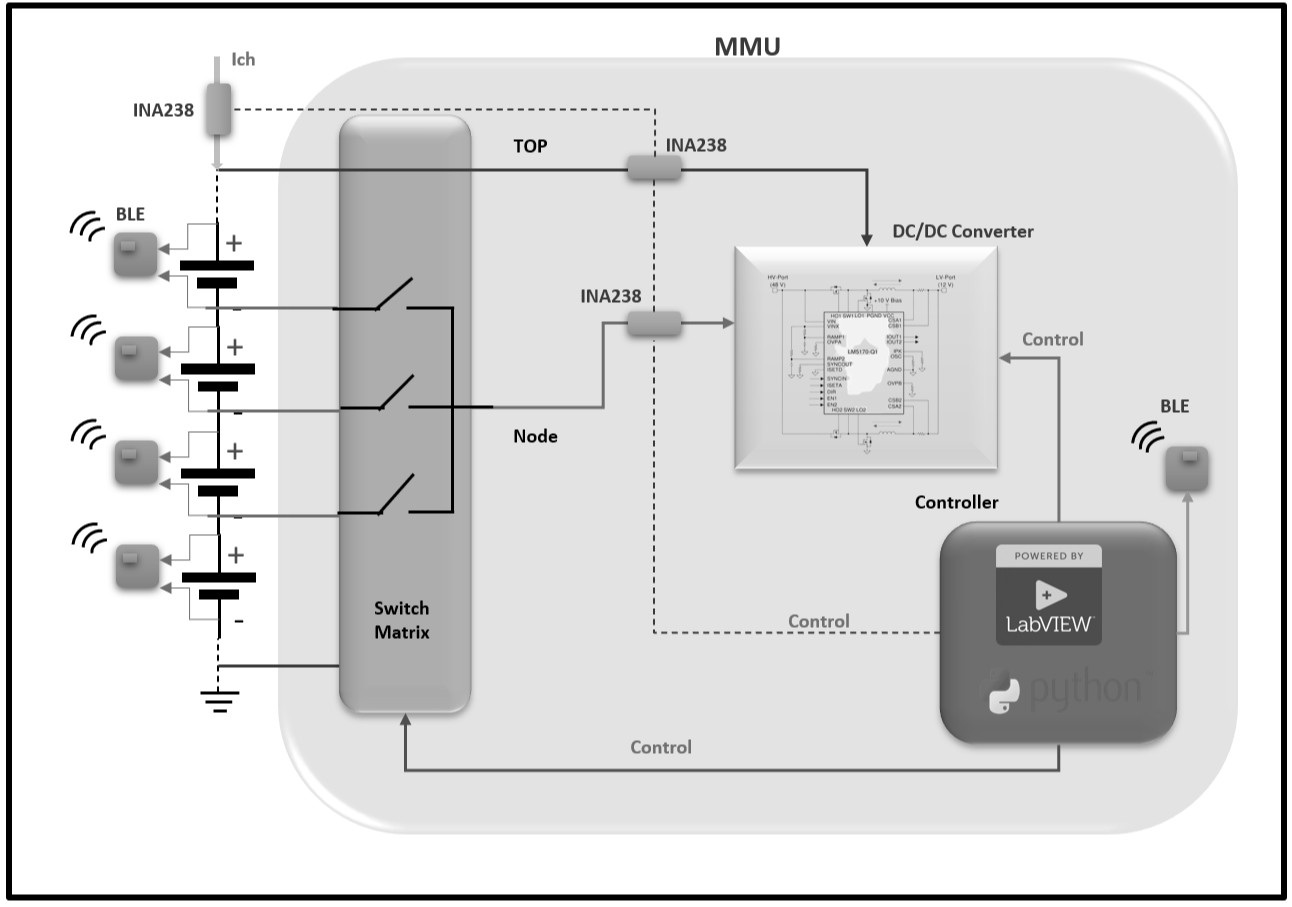
\includegraphics[width=0.8\paperwidth]{BMS_Architecture_border-modified.PNG}
  }%
}
\renewcommand{\thesubsubsection}{\thesubsection.\alph{subsubsection}}
\setcounter{secnumdepth}{4}

%\usepackage{subfigure}
\usepackage[ruled,linesnumbered,slide,vlined]{algorithm2e}
\SetKwProg{Init}{init}{}{}

%\usepackage{verbatim}
%\usepackage{wrapfig}
%\usepackage{multirow}


%% % % % % % %
\onehalfspacing
\begin{document}
\sloppy
% % % % % % % % % % % % % % % % % % % % % % % % % % %
% % % % % % % % % % % % % % % % % % % % % % % % % % %
\author{Harish Kumar Shivaramappa}

\authorGender{male}		
\department{Department of Electrical, Computer and Biomedical Engineering}
\docTitle{SOC and SOH estimation in BMS based on Wireless Communication Network}

% % % % % % % % % % % % % % % % % % % % % % % % % % % % % %
% % % % % % % % % % % % % % % % % % % % % % % % % % % % % %
% % %
\studentType{Master}			

	
% % % % % % % % % % % % % % % % % % % % % % % % % % % % % %
% % % 


\degree{Master of Science} 				     %%Master of Science; 


% % % % % % % % % % % % % % % % % % % % % % % % % % % % % %
% % % % % % % % % % % % % % % % % % % % % % % % % % % % % %

% % % Mention the discipline in which the degree is awarded
\degreeIn{Microelectronics}		


% % % % % % % % % % % % % % % % % % % % % % % % % % % % % %
% % % % % % % % % % % % % % % % % % % % % % % % % % % % % %

\docType{1}		%%Dissertation=1; Thesis=2; Project=3; Synopsis=4; Registration Report=5

% % % % % % % % % % % % % % % % % % % % % % % % % % % % % %
% % % % % % % % % % % % % % % % % % % % % % % % % % % % % %

\numOfSupervisors{2}

\principalSupervisor{Piero Malcovati}	%%Name only
\coSupervisor{Domenico Granozio}			%%Name only
\principalSupervisorDesignation{Professor}
% \coSupervisorDesignation{Eng}

% % % % % % % % % % % % % % % % % % % % % % % % % % % % % %
% % % % % % % % % % % % % % % % % % % % % % % % % % % % % %

% Just for the Sample Date 
\setDate{20}
\setMonth{December}
\setYear{2022}

% % % % % % % % % % % % % % % % % % % % % % % % % % % % % %
% % % % % % % % % % % % % % % % % % % % % % % % % % % % % %

\Font{1}	%% Times New Roman=1; Arial=2;
\setFont

% % % % % % % % % % % % % % % % % % % % % % % % % % % % % %
% % % % % % % % % % % % % % % % % % % % % % % % % % % % % %
% % % 

\titlePageLineSpacing{2}
\titleWidth{.75}
\titleCoordinateX{0.13}
\titleCoordinateY{0.12}

% % % % % % % % % % % % % % % % % % % % % % % % % % %
% % % % % % % % % % % % % % % % % % % % % % % % % % %
% % % % % % % % % % % % % % % % % % % % % % % % % % %
	% %Fill details in "FrontPages.tex"
% % % % % % % % % % % % % % % % % % % % % % % % % % %
% % % % % % % % % % % % % % % % % % % % % % % % % % %
%%\coverPageSynReg		% %Needed for Synopsis Cover Page or 
						% %Registration Report Cover Page.
						% %To be used along with "\docType()".
						% %Use "\section{Introduction}\label{Guidelines}
Submission of a synopsis or extended abstract is one of the mandatory requirements before submitting a doctoral or master thesis. It is not just a longer version of an abstract. It is as good as a research paper that conveys the essence of the thesis without overlooking the importance of introduction and conclusion. A synopsis should include the following~\textemdash~
\begin{itemize}
	\item Introduction
	\item Aim
	\item Method
	\item Results
	\item Conclusion
	\item Limitations
	\item References
	\item Dissemination
\end{itemize}

\noindent A synopsis is a self-contained, capsule description of the thesis that must make sense all by itself. Typical length of a synopsis should be between 5 and 10. Pages must of A4 dimension with 25mm margin on all four sides. The entire dissertation must be written using only a single font including all the texts inside graphs, figures, block diagrams, etc. While writing captions of tables and figures, the font size should be decreased by one point. Similarly, the font size of bibliography and index should also be lessened by a point. Students are advised to use the following in the body text~\textemdash
\begin{itemize}
\item[] serif fonts like Times New Roman (TNR) of size 12pt \\
or \\
\textsf{sans-serif fonts like Arial of size 11pt}. 
\end{itemize}
Needless to say that the use of font should be uniform throughout. Headings, Titles \textit{etc.} should use fonts as given below in Table~\ref{tab-fonts}.
{
\linespread{1}
\begin{table}[h]
\centering
\caption{Font sizes to be used in the dissertation}
\begin{tabular}{l C{25mm} C{25mm} c} 
\toprule
{Item} & Arial & {TNR} & {Justification}\\
\midrule\midrule
Main Text & 11 normal & 12 normal & Justified \\
\midrule
Sub-sub Heading & 11 bold & 12 bold & Left \\
\midrule
Sub Heading & 13 bold & 14 bold & Left \\
\midrule
Heading$^{\#}$ & 16 bold & 17 bold & Left \\
\midrule
Chapter Title & 22 bold & 24 bold & Center \\
\midrule
Chapter Number & 16 bold & 17 bold & Left \\
\bottomrule
\multicolumn{4}{l}{$^{\#}$Add serial number with one decimal place.} 
\end{tabular}
\label{tab-fonts}
\end{table}
}
\par The class file \texttt{NITR.cls} can be used to prepare a synopsis. One needs to invoke the statement ``\texttt{\textbackslash synopsisCoverPage}'' in the main ``\texttt{.tex}'' file with ``\texttt{\textbackslash docType(4)}'' and all necessary data in the ``\texttt{FrontPages.tex}''. The text of the synopsis can be written in ``\texttt{./SynopsisText/SynopsisText.tex}''."
						% %Comment rest.
\coverPage
\titlePage
% \certificateOfExamination

%\certificateOneSupervisor		%% Comment any
% \certificateTwoSupervisors		%% one of these two

\dedication
% \declaration

\acknowledgment
\abstract
% % % % % % % % % % % % % % % % % % % % % % % % % % %
% % % % % % % % % % % % % % % % % % % % % % % % % % %
% \chapter*{Preface}
When started my Microelectronics master's program at the University of Pavia, I was wondering about the future of microelectronics in the domain of electric vehicle and sustainable energy management because I have witnessed personally how world leaders are crumbling to fix global warming and climate change. The idea of making global warming free through sustainable energy drove me to explore electrical vehicles and power management. As I was intensively researching my self about electrical vehicles and battery management systems, I got an opportunity to enroll LM+ program at the university of Pavia which is doing an internship through the university in corporate companies for one year.\\
\indent Among the LM+ opportunities, I have noticed that Inventvm a dynamic young Italian company is doing research on Battery management systems for electrical vehicles. Since my interest is to work in power management and sustainable energy management, the Inventvm BMS project became a cherry on the pie for me. During the process, I met Eng. Domenico (Inventvm project BMS project manager), his idea of an elaboration made me more curious about the project and I stretched my legs immediately to the Inventvm on Feb 2020.\\
\indent As I was stepping into Inventvm I started to experience the radiation of the knowledge from the engineers because they are not kids like me. As a young rookie in technology, I start to learn more about the hardware and software of the project because the bus(project) is already started way before I join to the company. That was ok! because at the age of 10 I smoked the LED placing it in 230V mains, what ??????? YES that's right, for sure the led did not glow bright, but my brain became to dig into why LED got burned despite the black smoke on the face while LED burned. Anyway, later I was educated by my father(of course he is an electrician) that LED needs some kind of electronic circuit to make it glow. when my father made LED glow, That was WoW, "astonishing"! LED was not too much bright enough though. This idea of making education by failure became fascinating this same strategy worked for me to understand this in the industry too quickly not to miss the bus. There are always my colleagues who gave me a shoulder to shoulder when I was stuck in some technological part.\\
\indent Before my Master's, I worked with Analog Device Inc as IoT application Engineer and System Testing Engineer for Highpower circuits in NEXTGEN computers. The knowledge gained from these two institutions, helped in my current project to understand the Wireless communication environment and power management. My experience in these two prime companies laid the foundation for analytical skills and problem-picking skills throughout the project. Nevertheless, the key motivation was my father and all my teachers who educated me throughout my life to contribute well to nature and humanity. Nonetheless, \textit{Prof. Malcovati} has been a gem among all my honorable teacher's treasury who shined bright in my way. Thanks......!
% \thispagestyle{empty}
% \cleardoublepage
% % % % % % % % % % % % % % % % % % % % % % % % % % %
% % % % % % % % % % % % % % % % % % % % % % % % % % %
\tableofcontents
\cleardoublepage
% % % % % % % % % % % % % % % % % % % % % % % % % % %
% % % % % % % % % % % % % % % % % % % % % % % % % % %
\addcontentsline{toc}{chapter}{List of Figures}
\listoffigures
\cleardoublepage
% % % % % % % % % % % % % % % % %
\addcontentsline{toc}{chapter}{List of Tables}
\listoftables
\cleardoublepage
% % % % % % % % % % % % % % % % % % % % % % % % % % %
% % % % % % % % % % % % % % % % % % % % % % % % % % %
\pagenumbering{arabic}
\pagestyle{fancy}
\renewcommand{\chaptermark}[1]{\markboth{#1}{}}
\renewcommand{\sectionmark}[1]{\markright{\textbf{Chapter \thechapter}}}

% % % % % % % % % % % % % % % % % % % % % % % % % % %
% % % % % % % % % % % % % % % % % % % % % % % % % % %
\chapter*{Preface}
When started my Microelectronics master's program at the University of Pavia, I was wondering about the future of microelectronics in the domain of electric vehicle and sustainable energy management because I have witnessed personally how world leaders are crumbling to fix global warming and climate change. The idea of making global warming free through sustainable energy drove me to explore electrical vehicles and power management. As I was intensively researching my self about electrical vehicles and battery management systems, I got an opportunity to enroll LM+ program at the university of Pavia which is doing an internship through the university in corporate companies for one year.\\
\indent Among the LM+ opportunities, I have noticed that Inventvm a dynamic young Italian company is doing research on Battery management systems for electrical vehicles. Since my interest is to work in power management and sustainable energy management, the Inventvm BMS project became a cherry on the pie for me. During the process, I met Eng. Domenico (Inventvm project BMS project manager), his idea of an elaboration made me more curious about the project and I stretched my legs immediately to the Inventvm on Feb 2020.\\
\indent As I was stepping into Inventvm I started to experience the radiation of the knowledge from the engineers because they are not kids like me. As a young rookie in technology, I start to learn more about the hardware and software of the project because the bus(project) is already started way before I join to the company. That was ok! because at the age of 10 I smoked the LED placing it in 230V mains, what ??????? YES that's right, for sure the led did not glow bright, but my brain became to dig into why LED got burned despite the black smoke on the face while LED burned. Anyway, later I was educated by my father(of course he is an electrician) that LED needs some kind of electronic circuit to make it glow. when my father made LED glow, That was WoW, "astonishing"! LED was not too much bright enough though. This idea of making education by failure became fascinating this same strategy worked for me to understand this in the industry too quickly not to miss the bus. There are always my colleagues who gave me a shoulder to shoulder when I was stuck in some technological part.\\
\indent Before my Master's, I worked with Analog Device Inc as IoT application Engineer and System Testing Engineer for Highpower circuits in NEXTGEN computers. The knowledge gained from these two institutions, helped in my current project to understand the Wireless communication environment and power management. My experience in these two prime companies laid the foundation for analytical skills and problem-picking skills throughout the project. Nevertheless, the key motivation was my father and all my teachers who educated me throughout my life to contribute well to nature and humanity. Nonetheless, \textit{Prof. Malcovati} has been a gem among all my honorable teacher's treasury who shined bright in my way. Thanks......!
\thispagestyle{empty}
\cleardoublepage
% % % % % % % % % % % % % % % % % % % % % % % % % % %
% % % % % % % % % % % % % % % % % % % % % % % % % % %
%%%%%%%%%%Introduction %%%%%%%%%%%%%%%%%%%%%%%%%%%%%%
%Formatting Guidelines for Writing Dissertation.
\chapter*{Introduction}\label{intro}

\ \ \ \ \ \ \  
\thispagestyle{empty}
\cleardoublepage
% % % % % % % % % % % % % % % % % % % % % % % % % % %
% % % % % % % % % % % % % % % % % % % % % % % % % % %
%Some Unstructured Advice on Dissertation Writing
\chapter{Literature Survey}\label{literature_survey}

I will summarize Literature Survey soon.



\thispagestyle{empty}
\cleardoublepage
% % % % % % % % % % % % % % % % % % % % % % % % % % %
% % % % % % % % % % % % % % % % % % % % % % % % % % %

\chapter{Bluetooth Module Design}\label{chap:BLE}
% \stepcounter{chapter}\addcontentsline{toc}{chapter}{Incremental Sigma-Delta Modulator}

\section{Introduction}


Antenna design and analysis are crucial in a wireless network that transmits and receives information through electromagnetic wave radiation in open space.
Modern Antenna and RF design techniques are more often testified against size, power, flexibility, radiation patterns, efficiency, etc...
It is very unusual to use a wide variety of RF fundamental design techniques even though the usage of silicon and power is different because the fundamentals of RF design are most rigorous and robust from decades, hence RF fundamentals and design techniques remain intact. Nevertheless, modern RF applications demand to emphasize efficiency and power requirements, so this requirement needs some special RF Design treatments.
Chapter .3 gives the extravagance of PCB antenna design practices, general guidelines for grounding, PCB stacking, spacings and via holes, etc. Matching networks in RF design are extremely important to increase the efficiency of the Antenna and RF line, so it is also explored in the same chapter how to pick the passive components for RF Antenna matching such as capacitors and inductors.

%%%%%%*********************************************************%%%%%%%
%%%%%%*************************New Section*********************%%%%%%%
%%%%%%*********************************************************%%%%%%%
\section{Antenna Basics :}

An Antenna is a piece of metal exposed to free space. A piece of conductor behaves like an antenna when its length is a certain ratio or multiple of the wavelength of the signal. This scenario is expressed as "resonance", where the antenna radiates the electrical energy to the open space.




\begin{figure}[h]
	\centering
	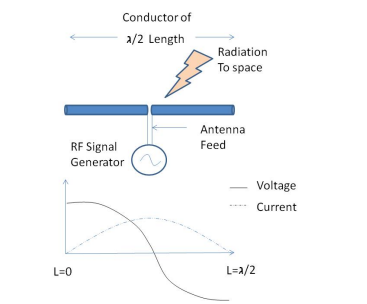
\includegraphics[width=0.7\textwidth]{Chap03/Figures/Basic_Antenna.PNG}
	\caption{Basic dipole Antenna}
	\label{BASIC_ANTENNA}
\end{figure}

Fig.1  shows the dipole antenna whose length is  $\lambda/2$ and the fed has an input impedance of $50\Omega $.
Dipole antennas are the most basic antennas that have been used for broadcasting.
In the Millennial age of technology, dipole antennas have been bulky and heavy, thanks to the PCB technology, which made dipole antennas extremely simple in construction and this became the center of attraction for the Bluetooth application in the modern era.
Although dipole antennas are extremely comfortable for PCB we still face hurdles to manage proper grounding for the antenna..which can be addressed through quarter-wave antennas.
The quarter-wave antennas have half of the length of the dipole antennas  $\lambda/4$, their popularity became exponential because of the fed which can be single-ended.
A single-ended feed to the antenna made life much easier to make a wide range of ground planes and better matching.

%%%%%%%%%%%%%%%%%%%%%%%%%%%%%%%%%%%%%%%%%%%%%%%%%%%%%%%%%%%%%%%%%%%%%%%%%%%%%%%%%%%%%
\subsection{Antenna Types:}

As discussed in the previous section quarter wavelength antennas can be more effective on the PCB because of their fed and ground plane management on PCB.
Depending on the antenna dimensions and the shape of antennas fall into different technologies namely FM, AM, Bluetooth, Wi-Fi and so on.
Since the eccentric part of this chapter discusses the Bluetooth antenna design and guidelines, we can broadly classify three types of antennas. As follows :

\subsubsection{Wire Antenna :}
These types of antennas are just a piece of wire extended over the PCB in open space, whose length is matched to $\dfrac{\lambda}{4}$ on the ground plane.
In general, these antennas are fed by a $50\Omega  $ matching transmission line, a Wire antenna gives a top-notch performance and supports a wide range of frequencies because of its three-dimensional exposure in open space.
The shape of the wire antennas can be loop, wire, or helix.. depending on the application the shape is changed.

\begin{figure}[h]
	\centering
	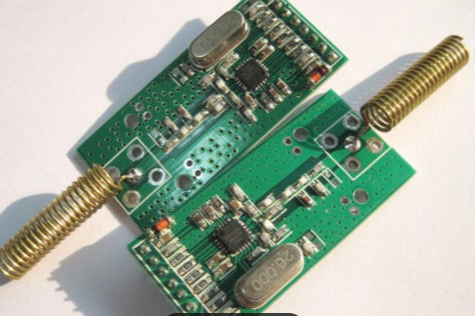
\includegraphics[width=0.4\textwidth]{Chap03/Figures/Wire_antenna.PNG}
	\caption{Wire Antenna}
	\label{WIRE_ANTENNA}
\end{figure}


\subsubsection{ PCB Antenna :}Constructively this type of antenna is copper traces
that are etched on the PCB. The Traces can be Zig-Zag, straight, MIFA, Meandered type, F-type, or Zip track so on.,
the shape of the antenna is chosen based on the antenna type and the space constraints on the PCB. PCB Antennas have only two-dimensional freedom, therefore certain guidelines are needed for the PCB antenna design due to the space constraints and poor quality of PCB stack-up.
The space constraints of the PCB antennas lead to less efficiency compared with wire antennas nonetheless PCB antennas are cost-effective.
In short manufacturing comfortability and its wireless range is ravishing for Bluetooth applications.

\begin{figure}[h]
	\centering
	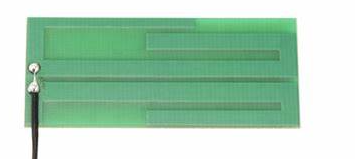
\includegraphics[width=0.4\textwidth]{Chap03/Figures/PCB_Antenna.PNG}
	\caption{PCB Antenna}
	\label{PCB_ANTENNA}
\end{figure}


\subsubsection{ Chip Antenna :} This is a Small form factor IC that is in-house with a ceramic package or some metal case.
These antennas are handier in terms of space management on the board and internally their impendence is very well managed.
A chip antenna can also take an advantage of three-dimensional freedom for radiation similar to wire antennas.
Refer to figure 10 for the Nordic Bluetooth module having a chip antenna.
Chip antennas can indeed gain upper hand in size and radion pattern on the contrary power handling capacity of the chip antenna is very minimal.
\begin{figure}[h]
	\centering
	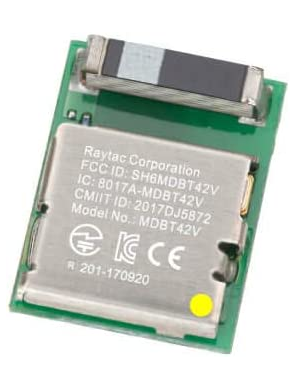
\includegraphics[width=0.4\textwidth]{Chap03/Figures/Chip_Antenna.PNG}
	\caption{Chip Antenna}
	\label{CHIP_ANTENNA}
\end{figure}



\subsection{Antenna Parameters}

The following section gives some key antenna performance parameters.

\subsubsection{Return loss :}

The return loss of an antenna signifies how well the antenna is matched to the 50-Ω transmission line (TL), shown as a signal feed in Figure \ref{fig: ANTENNA_RETUNRNLOSS}. The TL characteristic impedance is typically 50 Ω, although it could be a different value. The industry standard for commercial antennas and testing equipment is 50-Ω impedance, so it is most convenient to use this value \cite{AN91445}. \\
	
\indent  Return loss indicates how much of the incident power is reflected by the antenna due to mismatch (Equation \ref{eq:Antenna_Returnloss}).
An ideal antenna when perfectly matched will radiate the entire energy without any reflection. If the return loss is infinite, the antenna is said to be perfectly matched to the TL, as shown in Figure \ref{fig:ANTENNA_RETUNRNLOSS}. S11 is the negative return loss expressed in decibels. In most cases, a return loss ≥ 10 dB (equivalently, S11 ≤ –10 dB) is considered sufficient. Table \ref{tb:ANTENNA_RETURNlOSS_TABLE} relates the return loss (dB) to the power reflected from the antenna (percent). 
A return loss of 10 dB signifies that $90\%$ of the incident power goes into the antenna for radiation \cite{AN91445}.

\begin{equation}\label{eq:Antenna_Returnloss}
    \begin{split}
        Returnloss(db) = 10 \times \log( \frac{Pincident}{Preflected})
    \end{split}
\end{equation}

\begin{figure}[h]
	\centering
	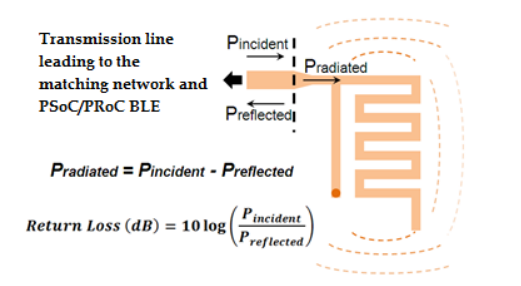
\includegraphics[width=0.65\textwidth]{Chap03/Figures/Antenna_ReturnLoss.PNG}
	\caption{Antenna Return loss}
	\label{fig:ANTENNA_RETUNRNLOSS}
\end{figure}

\begin{table}[h]
	\begin{tabular}{|c|c|c|c| }
		\hline 
		S11 (dB) & Return Loss (dB) & $\varGamma_{ref}$/$\varGamma_{inc}$ $(\%)$ & $\varGamma_{rad}$/$\varGamma_{inc}$ (\%) \\ 
		\hline
		–20 &20 &1 &99\\
		\hline
		–3 &3 &50 &50\\
		\hline
		–10 &10 &10& 90\\
		\hline
		–1 &1 &79 &21\\
		\hline
	\end{tabular}
	\caption{Return Loss and Power reflected from antenna}
	\label{tb:ANTENNA_RETURNlOSS_TABLE}
\end{table}



\subsubsection{Bandwidth :}

Bandwidth indicates the frequency response of an antenna. It signifies how well the antenna is matched to the 50-Ω transmission line over the entire band of interest, that is, between 2.40 GHz and 2.48 GHz for BLE applications \cite{AN91445}.\\

	\begin{figure}[h]
		\centering
		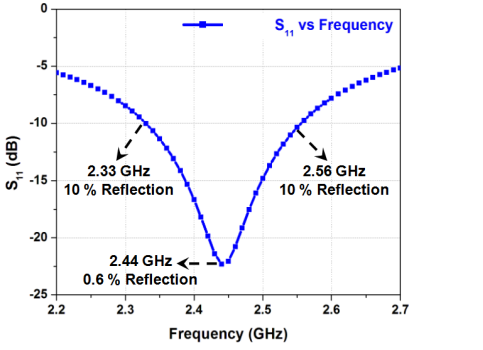
\includegraphics[width=0.65\textwidth]{Chap03/Figures/Antenna_Bandwidth.PNG}
		\caption{Antenna Bandwidth}
		\label{fig:ANTENNA_BANDWIDTH}
	\end{figure}

As Figure \ref{fig:ANTENNA_BANDWIDTH} shows, the return loss is greater than 10 dB from 2.33 GHz to 2.55 GHz. Therefore, the bandwidth of 
interest is around 200 MHz. Wider bandwidth is preferred in most cases, because it minimizes the effect of detuning 
resulting from the changes in the environments around the antenna in actual uses of the product (e.g. mouse placed 
on wood/metal/plastic table, hand kept around the mouse, etc.) \cite{AN91445}

\subsubsection{Radiation efficiency: }

A portion of the non-reflected power (see Figure \ref{eq:Antenna_Returnloss}) gets dissipated as heat or as thermal 
loss in the antenna. Thermal loss is due to the dielectric loss in the FR4 substrate and the conductor loss in the 
copper trace. This information is characterized as radiation efficiency. The radiation efficiency of 100 percent indicates 
that all non-reflected power is radiated to free space. For a small-form-factor PCB, the heat loss is minimal \cite{AN91445}.

\subsubsection{Radiation pattern:}
Radiation pattern indicates the directional property of radiation, that is, which directions have 
more radiation and which have less. This information helps to orient the antenna properly in an application \cite{AN91445}.\\


\indent An isotropic dipole antenna radiates equally in all directions in the plane perpendicular to the antenna axis. However, 
most antennas deviate from this ideal behavior. See the radiation pattern of a PCB antenna shown in Figure \ref{fig:ANTENNA_RADIATION_PATTERN} as an 
illustration. Each data point represents RF field strength, measured by the received signal strength indicator (RSSI) in 
the receiver. As expected, the contours are not exactly circular, as the antenna is not isotropic \cite{AN91445}.


\subsubsection{Gain :}
Gain indicates the radiation in the direction of interest compared to the isotropic antenna, which radiates 
uniformly in all directions. This is expressed in terms of dBi—how strong the radiation field is compared to an ideal 
isotropic antenna \cite{AN91445}.

\begin{figure}[h]
	\centering
	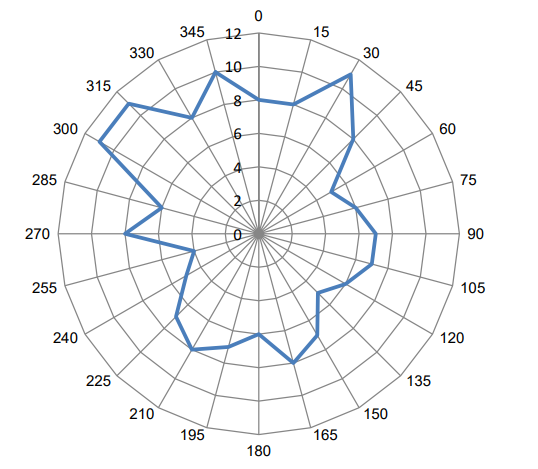
\includegraphics[width=0.65\textwidth]{Chap03/Figures/Antenna_Radiation_Pattren.PNG}
	\caption{Antenna Radiation Pattren}
	\label{fig:ANTENNA_RADIATION_PATTERN}
\end{figure}


\section{Motivation for Designing BLE Modules }
One of the core ideas of the Inventvm BMS team is to make the BMS project in a wireless communication environment, therefore the team has decided to use Bluetooth as the communication tool. Hence, finding the big sharks (Bluetooth Hardware and stack) in the Bluetooth world took quite some time, after a long investigation; we concluded to pick two important pies in the Bluetooth cake such as STM BLUeNRG-355mc \cite{BLNRG355_STEVAL_GUIDE} and Nordic nRF52840 \cite{NORDIC_nrf52840_USERGUIDE}. BlueEnergy-355mc is the jewel of our projects because it owes the advantages of very low power consumption: 3.4 mA, Receiver sensitivity, Bluetooth low energy data extensions, high data rate so on... despite having these many advantages STM does not manufacture the Bluetooth modules other than eval boards. Henceforth, the team has been paralyzed to outsource the required Bluetooth modules, later in the same path we found MIDARTRONICS the company that manufactures the Bluetooth modules using the STM BLUeNRGgy-355mc hardware named STORMY. Stormy is a such cutie pie, at least it helps to some extent in R and D to prove the Wireless communication BMS architecture, but in the long run, we have experienced some the discomforts such as lack of documentation and market supply...to overcome all these issues team has decided to make inventive proprietary level Bluetooth modules for BMS project. This gave me the perfect timing and to opportunity design RF Bluetooth modules for the project, as part of my thesis which is dedicated to wireless communication BMS.\\
\indent Nordic nRF52840\cite{NORDIC_nrf52840_USERGUIDE} is another Bluetooth hardware similar to the BlueEnergy-355Mc reason behind picking the Nordic is the open BLE stack and Robust hardware. Nordic is much more comfortable in terms of different data rates, on-chip power converters, 32-bit ARM Cortex M4F @64MHz so and forth. Nordic has also a dedicated BLE stack \cite{NORDIC_nrf52840_SOFTWARESTACK_GUIDE} that handles all power management resources on-chip, which attracts low-power automobile applications. In a much broader sense, Nordic is additional Bluetooth hardware that we can provide to the customer according to the application's need.\\
\indent Though picking the Bluetooth hardware and stack is a boiling task, choosing the antenna and RF layout also takes prime place. Though, there are plenty of antennas for the 2.4GHz band, most Bluetooth manufacturers recommend two types of PCB antennas, meanders inverted antennas (MIFA) and inverted-F antenna (IFA), which are characterized and simulated exclusively for the low-power Bluetooth applications. However, MIFA (PIFA) is peculiar for most automobile applications because of its pointed directional properties.\\
\indent, However, we can choose any type of antenna and hardware for Bluetooth, admittedly the antenna, hardware, and RF layout design described in the following modules are classified for the BMS project.\\
\indent The Low Data rate and bandwidth requirement in Bluetooth applications make IFA and MIFA the two most atractive antennas for BLE.  Manufacturing these antennas is extremely easy because they are part of the PCB design. Certainly, these antennas are inexpensive as they are part of PCB and they provide good bandwidth in ranges for BLE in terms of 150 to 250 MHZ.MIFA is most preferable for smaller form factor PCBs such as a wireless mouse, wearable watches, handy IoT devices.... etc. IFA antennas are recommended for applications such as one of the dimensions is needed to be smaller than the other for example heart rate monitor.
The following modules explain MIFA and IFA antennas construction and functionalities:

\section{PCB Meandered Inverted-F Antenna (PIFA/MIFA)}

PIFA antennas are much more popular in Bluetooth Low Energy stack because of the small size, low profile and cost-effective compared to the conventional dipole and ceramic chip antennas.
The proposed structure (PIFA/MIFA) Figure \ref{fig:MIFA_Antenna_1} of the PIFA antenna is routed to gain all these advantages.
Replacing the conventional PCB trace in PIFA with the meandering line and meandering shorting strip
improves the efficiency of the PIFA as well as the bandwidth. 
\begin{figure}[h]
	\centering
	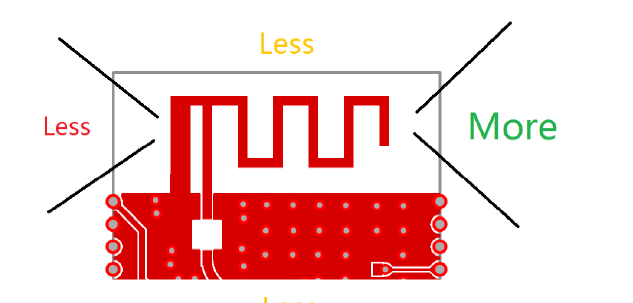
\includegraphics[width=0.4\textwidth]{Chap03/Figures/MIFA_Antenna_radiation_direction.PNG}
	\caption{MIFA/PIFA antenna radiation direction}
	\label{fig:MIFA_RADIATION_DIRECTION}
\end{figure}

Figure \ref{fig:MIFA_Antenna_1} Taking the meandered shape on one side and connecting meandered terminal to the ground makes the radiation lobe a more directional Figure\ref{fig:MIFA_RADIATION_DIRECTION} that implicates the radiation of the meandered antenna.Meandered side of the antenna radiates very less power because the Menderes terminal is connected to the ground which nullifies most of the radiation on the backward side. This kind of feature is highly needed in extremely noisy environments such as automobiles, power grid applications, data servers....etc.
As a case study, the design and measurement results of the
proposed MIFA/PIFA are presented \cite{PIFA2017Cheuk} in Figure\ref{fig:MIFA_Antenna_1}.


\begin{figure}[h]
	\centering
	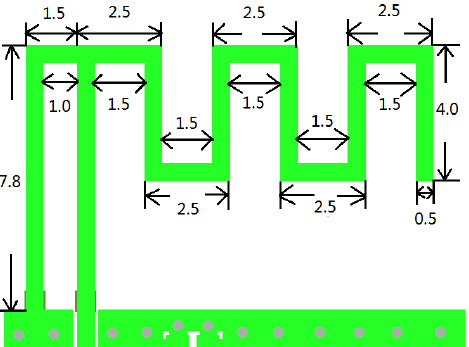
\includegraphics[width=0.65\textwidth]{Chap03/Figures/MIFA_Antenna.PNG}
	\caption{PCB Inverted Meandered F type Antenna \cite{NXP_AN11994_Antenna_Guide} }
	\label{fig:MIFA_Antenna_1}
\end{figure}

\subsection{Antenna used in Inventvm BLE modules :}
\indent I got an opportunity complete the Inventvm BLE module antenna simulation Figure\ref{fig:MIFA_Antenna_1} to depict the typical board shape and the antenna placement \cite{NXPBLE_Antenna_Guide}. The RF shield housing has been removed for testing purposes, usually, Bluetooth modules provide RF housing to protect the BLE from external interference.

\begin{figure}[h]
	\centering
	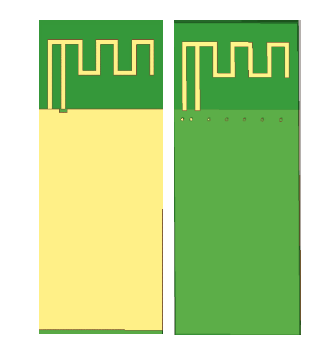
\includegraphics[width=0.4\textwidth]{Chap03/Figures/mifa_antenna_pcb_example.PNG}
	\caption{BLE module PCB with the MIFA/PIFA antenna placement}
	\label{fig:fig:PIFA_Antenna_PCB}
\end{figure}

Some MIFA/PIFA antenna and PCB parameters that are used for the simulation are shown in the table \ref{tb:MIFA_ANTENNA_SIMULATION_PARAMETERS}.

\begin{table}[h]
	\centering
	\begin{tabular}{|c|c|c| }
		\hline 
		\textbf{Antenna parameters} & \textbf{Value} & \textbf{Unit} \\ 
		\hline
		PCB substrate permittivity & 4.6 & — \\
		\hline
		PCB substrate H & 1.0 & mm \\
		\hline
		Length of PCB substrate & 35.5 &mm\\
		\hline
		Width of PCB substrate &14 &mm\\
		\hline
		Length of TOP PCB ground & 25.5& mm\\
		\hline
		Width of TOP PCB ground& 14& mm\\
		\hline
		Length of BOT PCB grounD &25.5 &mm\\
		\hline
		Width of BOT PCB ground &14 &mm\\
		\hline
		Width of antenna trace &0.5 &mm\\
		\hline
	\end{tabular}
	\caption{MIFA/PIFA antenna simulation parameters \cite{NXP_AN11994_Antenna_Guide}}
	\label{tb:MIFA_ANTENNA_SIMULATION_PARAMETERS}
\end{table}

\subsection{S11 of the MIFA/PIFA antenna}
Figure\ref{fig:MIFA_S11} shows the MIFA/PIFA antenna s11 parameter simulation results. The Bluetooth frequency bandwidth ranges from 2402 to 2483.5 MHz. The return loss of the antenna in the Bluetooth frequency band is less than the -10db.

\begin{figure}[h]
	\centering
	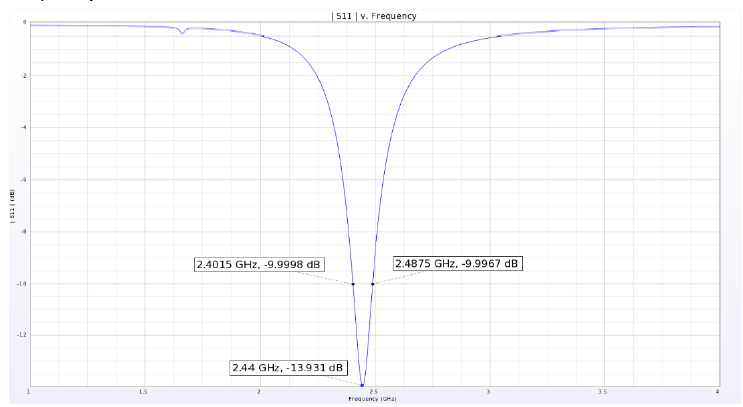
\includegraphics[width=0.7\textwidth]{Chap03/Figures/MIFA_Antenna_S11.PNG}
	\caption{MIFA/PIFA antenna S11 return loss}
	\label{fig:MIFA_S11}
\end{figure}
\begin{figure}[h]
	\centering
	\subfigure[MIFA antenna Gain Radiation pattern $@ \phi =90\deg$]{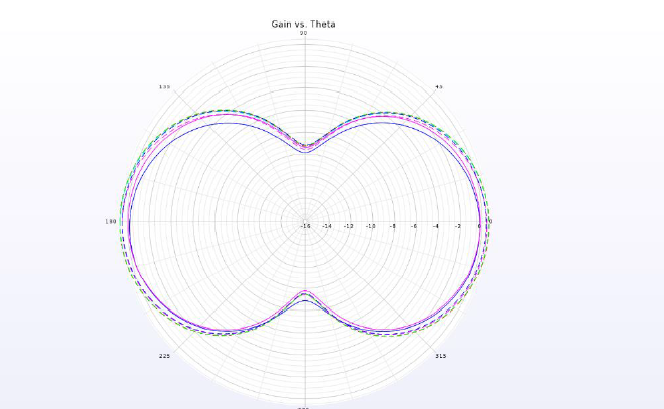
\includegraphics[scale=.5]{Chap03/Figures/mifa_Antenna_gain_pattern_phi_90.PNG}}
	\qquad
	\subfigure[MIFA antenna Gain Radiation pattern $@ \phi =0\deg$]{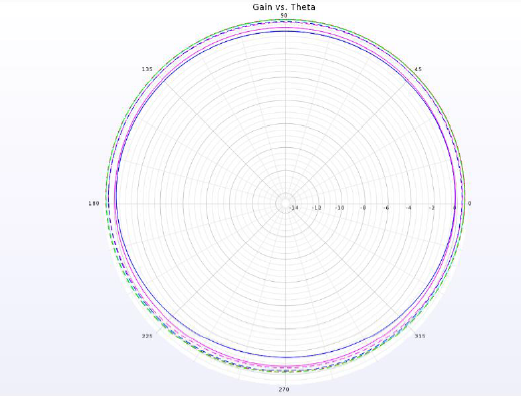
\includegraphics[scale=.5]{Chap03/Figures/mifa_Antenna_gain_pattern_phi_0.PNG}}
	\caption{MIFA Antenna Gain Radiation Pattren}
	\label{fig:MIFA_Antenna_Gain_Radiation_Pattren}
\end{figure}
\subsection{MIFA/PIFA antennas 3D pattern :}
\begin{figure}[h]
	\centering
	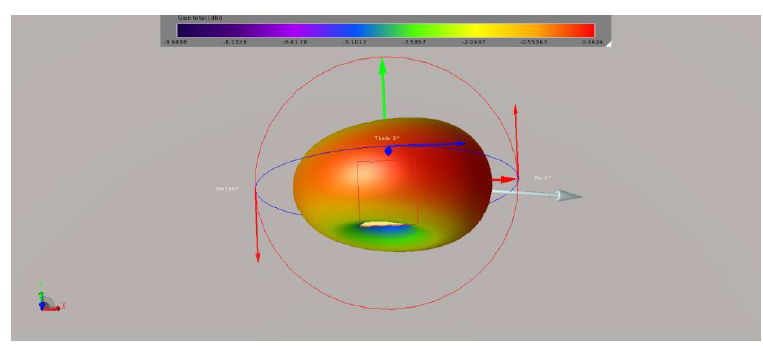
\includegraphics[width=0.7\textwidth]{Chap03/Figures/mifa_antenna_3d.PNG}
	\caption{MIFA/PIFA antenna 3D radiation Pattren}
	\label{fig:MIFA_3D}
\end{figure}

% \subsubsection{MIFA/PIFA antenna efficiency Simulation Results :}
\begin{figure}[h]
	\centering
	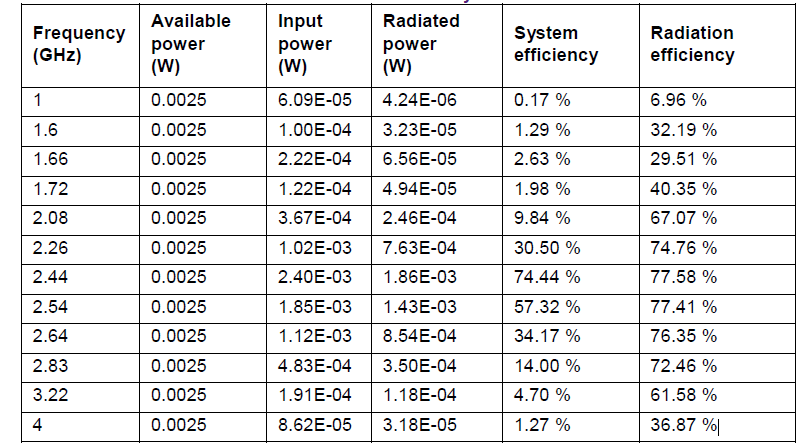
\includegraphics[width=1\textwidth]{Chap03/Figures/mifa_antenna_effieciency.PNG}
	\caption{MIFA/PIFA antenna efficiency Simulation Results}
	\label{fig:MIFA_antenna_effieciency}
\end{figure}

\section{Inverterd-F Antenna:}
The inverted F antenna is also one of the popular antennae, recommended for the Low power stack BLE applications. IFA antennas host similar features to what MIFA/PIFA antennas offer but MIFA antennas are more recommended where is a space constraint and power radiation is in one direction. IFA antennas have bidirectional power radiation rather than mono-directional. Nordic Recommends in all designs to use the IFA antennas. Figure \ref{fig:IFA_Antenna_1} educates the typical design of the IFA antenna and simulation parameters are pretty much the same as it is used for the MIFA antenna Table \ref{tb:MIFA_ANTENNA_SIMULATION_PARAMETERS}.

\begin{figure}[h]
	\centering
	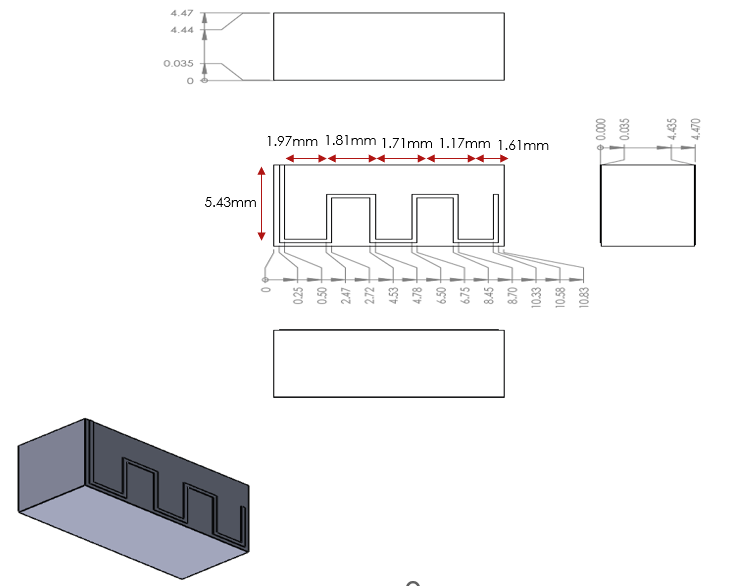
\includegraphics[width=1\textwidth]{Chap03/Figures/IFA_antenna.PNG}
	\caption{IFA antenna design and the placement}
	\label{fig:IFA_Antenna_1}
\end{figure}

By the constructional nature of the IFA antennas are easy to match we can see that in the Figure \ref{fig:IFA_Antenna_reflection} IFA antenna is very well-matched at 2.4GHz. The S11 is quite impressive because it has a reflection coefficient at 2.4GHz is -27db and bandwidth at -9db is 160MHz.
\begin{figure}[h]
	\centering
	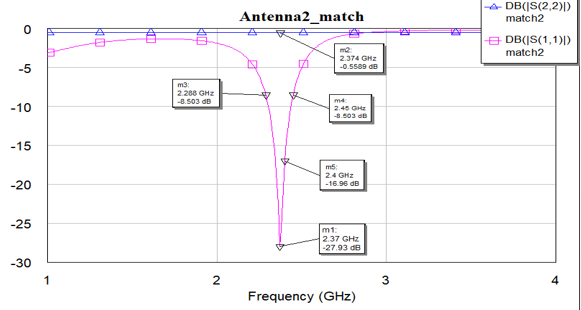
\includegraphics[width=1\textwidth]{Chap03/Figures/IFA_antenna_reflecctions.PNG}
	\caption{IFA antenna S11 and S22}
	\label{fig:IFA_Antenna_reflection}
\end{figure}
IFA antenna matching can be further tuned by varying the hinges, and length of the antennas, on contrary we need to compromise with power and resonant frequencies. Figure \ref{fig:IFA_S11_Change}shows the relative length and hinge width changes of the design Figure \ref{fig:IFA_Antenna_1} caused different frequency shfit, but they keep giving the best performance in matching.
\begin{figure}[h]
	\centering
	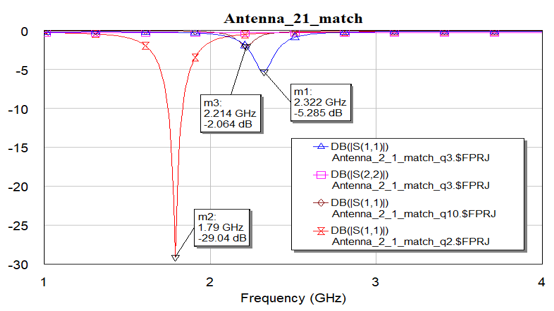
\includegraphics[width=1\textwidth]{Chap03/Figures/IFA_S11_Change.PNG}
	\caption{IFA antenna S11 Variation by changing the length and hinge width}
	\label{fig:IFA_S11_Change}
\end{figure}

% % % % % % % % % % % % % % % % % % % % % % % % % % %
% % % % % % % % % % % % % % % % % % % % % % % % % % %
\section{BLE Schematic and PCB layout}
The Schematic of the Inventvm BLE modules is inherited directly from the vendors, which are BluEnergy-355MC\cite{BLNRG355_STEVAL_GUIDE} and Nordic nRF52840\cite{NORDIC_nrf52840_USERGUIDE}. The Figure\ref{fig:Nordic_ST_modules} shows the pinout and shape of the BLE module, which is multi-purpose because of same shape and pinout from both the BluEnergy-355MC and Nordic nRF52840 modules. By having the Same pinout and shape with different Bluetooth hardware, customers can use different Bluetooth hardware stacks with the same BMS solution. This approach is nothing but the daughter and motherboard approach where the Bluetooth module becomes the daughter board and BMS MMU board and CMU boards become motherboards.

\begin{figure}[h]
	\centering
	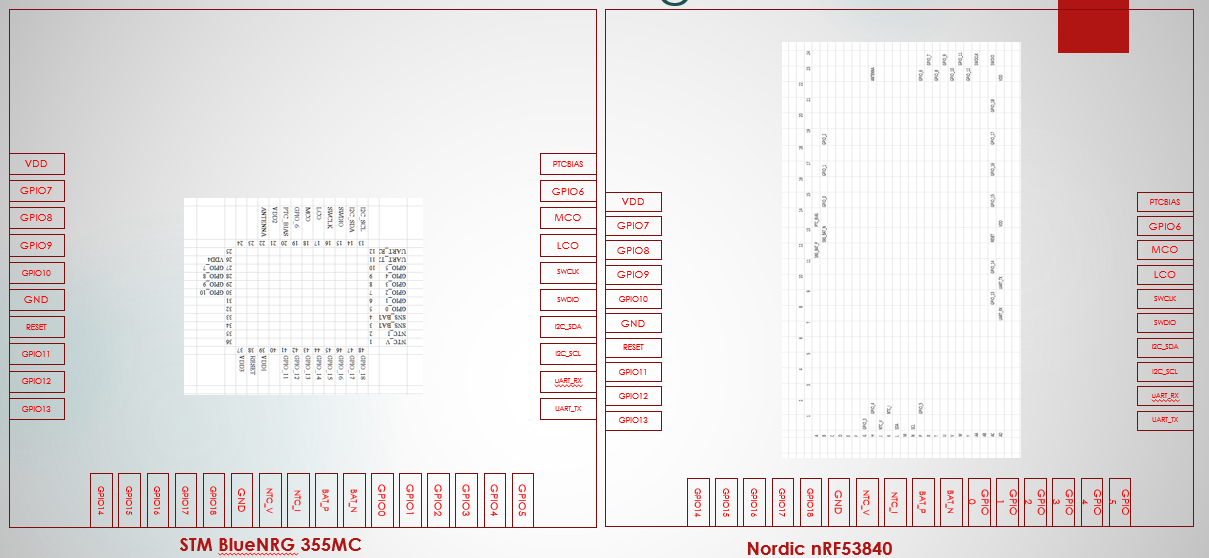
\includegraphics[width=0.7\textwidth]{Chap03/Figures/Nordic_ST_modules.PNG}
	\caption{BluEnergy-355MC(right) and Nordic Modules(left) }
	\label{fig:Nordic_ST_modules}
\end{figure}

\subsection{BluEnergy-355MC}
BLUENRG-355MC\cite{BLNRG355_STEVAL_GUIDE} BLE module includes BlueNRG-LP BLE low energy system on chip (QFN48 package), Associated with BlueNRG-LP development software stack from STM. The BlueNRG-LP features a 64 MHz, 32-bit Arm®Cortex®-M0+core, a 256 KB programmable flash memory, a 64 KB SRAM, an MPU, and an extensive peripheral set (6x PWM, 2x I²C, 2x SPI/I2S, SPI, USART, UART, PDM, and 12-bit ADC SAR)\cite{BLNRG355_STEVAL_GUIDE}. It is compliant with the Bluetooth® LE specification and supports master, slave, and simultaneous master-and-slave roles. It features data length extension, 2 Mbps, long-range, extended advertising and scanning, as well as periodic advertising, periodic advertising sync transfer, LE L2CAP connection-oriented channel, and LE power control and path loss monitoring\cite{BLNRG355_STEVAL_GUIDE}.
For more technical details refer STM BLUENRG-355MC datahseet \cite{BLNRG355_STEVAL_GUIDE}.
\subsubsection{BluEnergy-355MC RF Schematic:}
The Figure\ref{fig:STM_BLE_Schematic} refers to the core circuit of the BLUeNRG circuit for the Bluetooth, the pi network matching topology used to match the Ic and antennas, and refer \ref{fig:STM_BLE_Schematic} circuit between the RF net and the ANT net in the schematic.
All the discrete components are selected 0402 packages to make the Bluetooth module as sophisticated as possible, for more insight into the component selection for the schematic \ref{fig:STM_BLE_Schematic} refer to BOM\cite{BLNRG355_STEVAL_BOM}.
\begin{figure}[h]
	\centering
	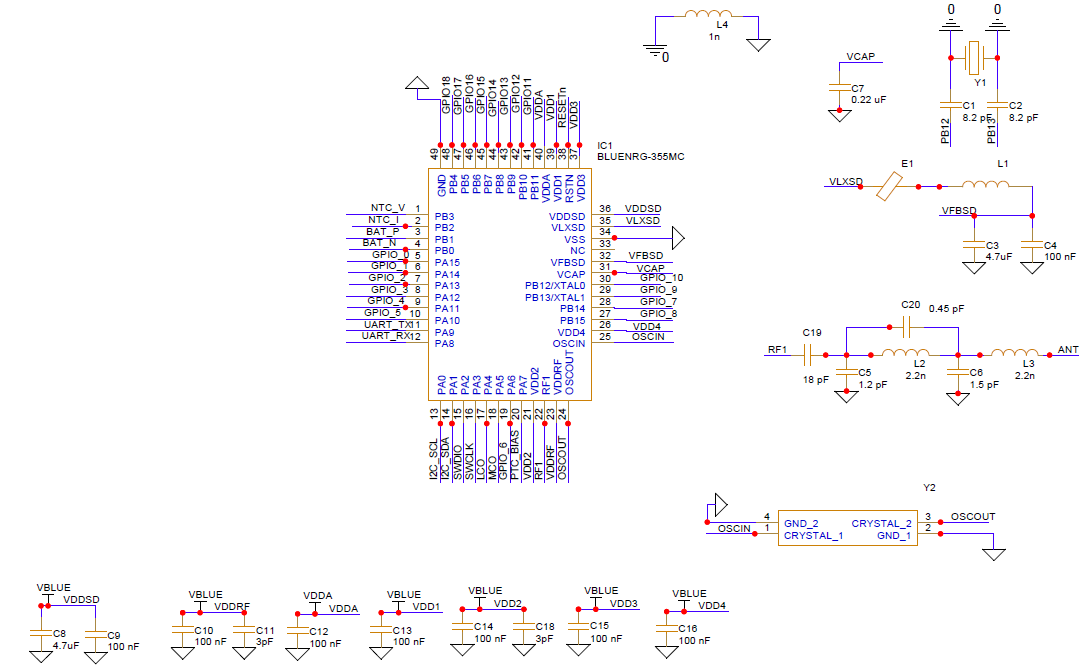
\includegraphics[width=0.7\textwidth]{Chap03/Figures/STM_BLE_Schematic.PNG}
	\caption{BluEnergy-355MC Module Core circuit }
	\label{fig:STM_BLE_Schematic}
\end{figure}

\subsubsection{BluEnergy-355MC RF Layout:}
The BLE module designed for the BMS application in Inventvm is the four-layer PCB, among four layers bottom layer is entirely dedicated to the ground. The bottom layer ground of the module is the analog ground it is differentiated from the power ground of the BMS from a small inductor to make sure the RF circuit gets less noise from the power ground. \\
\indent By referring to the layout Figure \ref{fig:BLE_PCB_ground_and_power_planes}of the RF module you can recognize that the shape of the power plane in the layer is pretty much weird, there is an RF technique behind making this kind of shape to avoid as much as the ground and power plane over a lap to decrease the capacitive parasitic effect. Parasitic components on PCB are the plague of the RF circuit, they can kill RF signal. Hence it is always a good idea to avoid power and ground planes overlap as much as possible and also make separate ground for the RF layout apart from the power ground.\\
\indent Place as many as vias possible from the top to bottom ground layer to enhance the ground layer capacity, and making sure to have equal space for antenna and RF feed line from the ground enhances the matching capability of the antenna. The following extinctions can give a detailed view of RF layout design:.

%%%%%%%%%%%%%%%%%%%%%%%%%%%%%%%%%%%%%%%%%%%%%%%%%%%%%%%%%%%%%%%%%%%%%%%%%%%%%%%%%%%%%%%%%%%%%%%%%%%%%%
%%%%% RF layout design guide lines 
%%%%%%%%%%%%%%%%%%%%%%%%%%%%%%%%%%%%%%%%%%%%%%%%%%%%%%%%%%%%%%%%%%%%%%%%%%%%%%%%%%%%%%%%%%%%%%%%%%%%%%

\begin{itemize}
	\item {\textbf{Power plane and Grounding :}}The power and Ground plane's overlap needs to be decreased as much as possible to avoid the parasitic capacitance effect. The Figure \ref{fig:BLE_PCB_ground_and_power_planes} refers to the power supply plane in the layer and the ground in the bottom layer.
		\begin{itemize}
			\noindent
			\begin{figure}[h]
				\centering
				\subfigure[Ground plane "Bottom layer"]{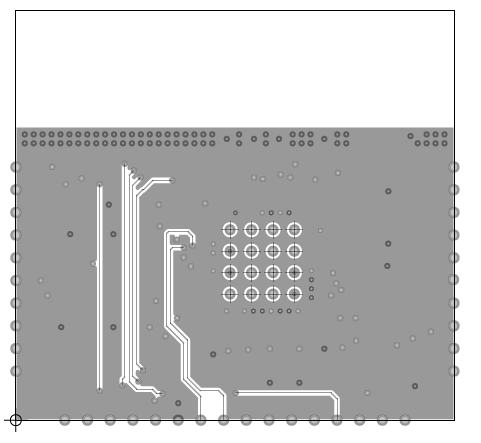
\includegraphics[scale=.6]{Chap03/Figures/nordic_module_grounding.PNG}}
				\qquad
				\subfigure[Power Plane "Layer 1"]{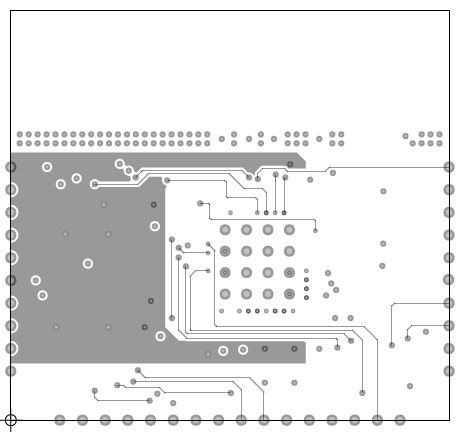
\includegraphics[scale=.6]{Chap03/Figures/Nordic_module_power_plane.PNG}}
				\caption{BLE PCB ground and power planes}
				\centering
				\label{fig:BLE_PCB_ground_and_power_planes}
			\end{figure}
		\end{itemize}
	\item \textbf{Equal Clearance to Antenna Feed :} It is essential to keep the same clearance throughout the RF feed line from the ground. This strategy helps to make equal parasitic capacitance from the ground. With an equal parasitic capacitance from the opposite side, the RF sanding wave reflections can be nullified. Figure\ref{fig:Antenna_Feed_clearence} depicts one such example of designing the RF feed line.
		\begin{itemize}
			\item \begin{figure}[h]
			    \centering
				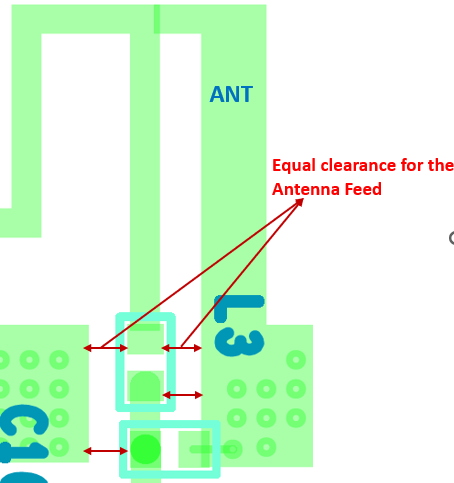
\includegraphics[width=0.4\textwidth]{Chap03/Figures/Antenna_Feed.PNG}
					\caption{Antenna Feed Line clearence}
					\label{fig:Antenna_Feed_clearence}
				\end{figure}
		\end{itemize}
	\item \textbf{ Isolate Power Ground from Analog/RF ground :}It is the most common practice while RF layout designing, The RF layout is isolated from the Power circuit. For this approach I have few intuitions behind the two-fold, those are :
		\begin{enumerate}\label{en:RFGND_isolation_benifits}
			\item RF-related noise is confined within the RF/Analog ground of the PCB.
			\item This will isolate noise from the digital circuitry with the DC power supply and High power switching circuit on the BMS board.
			\item RF circuit protected from direct current flow from DC supply if there are any power surges in supply. So on....
		\end{enumerate}
	    \begin{figure}[h]
			\centering
			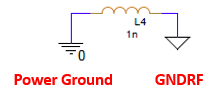
\includegraphics[width=0.4\textwidth]{Chap03/Figures/PGND_GNDRF_Isolation.PNG}
				\caption{Power Ground and RF Ground Isolated with Inductor}
				\label{fig:PGND_GNDRF_Isolation}
		\end{figure}
		\ref{en:RFGND_isolation_benifits} Such mentioned benefits can be obtained by placing an inductor between the Power Ground/RF ground. Choosing Inductor for such functionality follows that the inductor will not allow sudden current spikes $L\times \frac{d i}{d t}$ , on the benefit it can also provide a high current ratio when the current is stable,reference \ref{fig:PGND_GNDRF_Isolation}..
	\item \textbf{ RF feed line shape :}It is common practice to keep the rf feed line with the known shape. Since Bluetooth operates at 2.4GHz, even one millimeter can give a large amount of resonant frequency drift in antenna reflections. The simplest approach to mitigate such issues is to keep the RF feed and the RF IC, both on the same axis. To avoid unnecessary parasitics by an irregular shape of the antenna, make a feed trace from the ic to Antenna with the same width as the antenna feed has. Figure \ref{fig:Antenna_Feed_Shape} shows the approach that I have followed to design the Antenna feed and the RF trace, The Figure shows the nonregular shape of the antenna.
			\begin{itemize}
				\item 
				\begin{figure}[h]
					\centering
					\subfigure[Regular shape and Antenna feed]{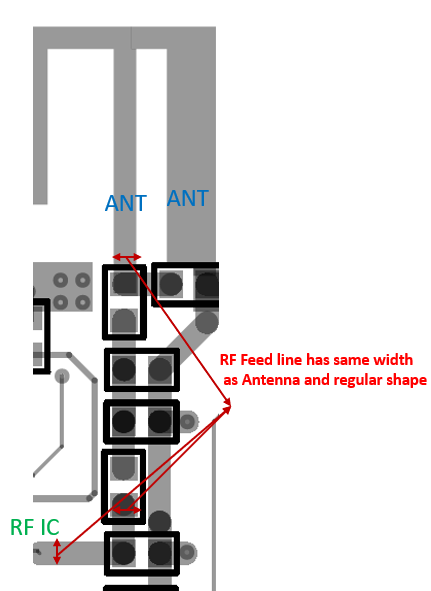
\includegraphics[scale=.6]{Chap03/Figures/Regular_Antenna_feed.PNG}}
					\qquad
					\subfigure[Irregular Antenna shape and Antenna feed]{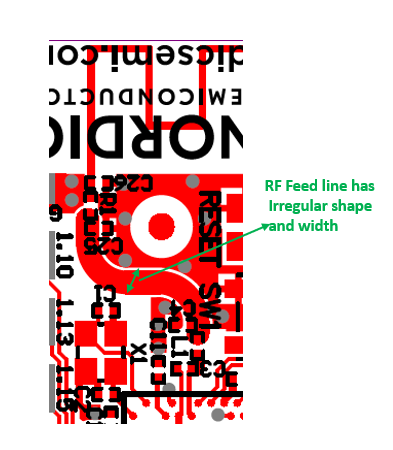
\includegraphics[scale=.6]{Chap03/Figures/Irregular_antenna_feed.PNG}}
					\caption{Antenna Feed Shape}
					\centering
					\label{fig:Antenna_Feed_Shape}
				\end{figure}
			\end{itemize}
	\item \textbf{Grounding Via's :} Keep always clean ground and this can be achieved by placing as many vias from the top layer to the dedicated RF/Analog ground in the bottom layer. It is recommended in the PCB design to place the Vias with equal distance, Figure \ref{fig:Antenna_Feed_Shape} refers to Vias placement from the top layer to the bottom layer with equal distance. There should not be any ground under the RF antenna, because the ground under the RF antenna again makes, Antenna just an RF trace instead of allowing open radiation.
	\begin{itemize}
		\item 
		\begin{figure}[h]
			\centering
			\subfigure[Top Layer Vias]{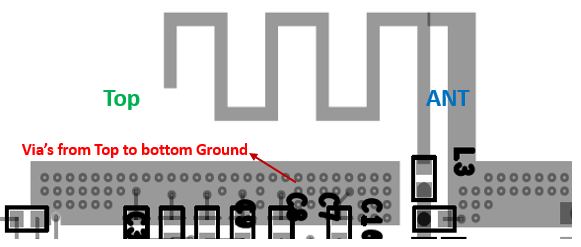
\includegraphics[scale=.5]{Chap03/Figures/Top_vias.PNG}}
			\qquad
			\subfigure[Bottom Layer Vias]{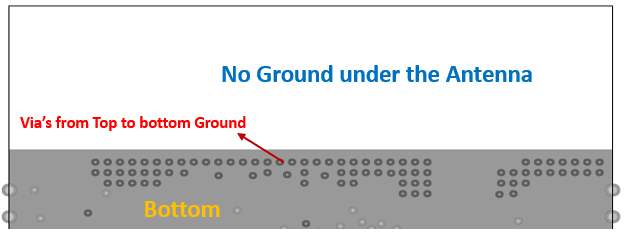
\includegraphics[scale=.5]{Chap03/Figures/Bottom_vias.PNG}}
			\caption{Vias placement on BLE board}
			\centering
			\label{fig:BLE_Module_Vias_Placement}
		\end{figure}
	\end{itemize} 
	\item \textbf{Antenna placement :} Do not place any component in the Antenna Keep out area, make the strict keep-out area for the antenna to prevent any external components' noise interference. It is always good placement to avoid any of the plastic components around the antenna because the plastic can behave like a dielectric and this will change the antenna characteristics. Antenna placement on they should end of the PCB where the PCB notch is pointed out. See Figure\ref{fig:BLE_PCB_ground_and_power_planes} the antenna has been placed on the edge of the PCB and there are no plastic or high-frequency switching circuits around it.
\end{itemize}

\subsubsection{Power Supply Decoupling Layout Considerations\cite{AN91445}}
Note the following best practices when laying out the power supply traces:
\begin{itemize}
	\item Place the components as close to the supply pin as possible \cite{AN91445}.
	\item Place the smallest-value capacitor closest to the power supply pin \cite{AN91445}.
	\item Place the decoupling capacitor on the same layer as the IC. If it is not possible to place all the capacitors on the same layer, give priority to smaller values \cite{AN91445}.
	\item The power supply should flow through the decoupling capacitors to the power supply pin of the IC. Avoid using
	\item supply vias between the component and the pin \cite{AN91445}.
	\item Use separate vias to ground for each decoupling capacitor. Do not share vias\cite{AN91445}.
	\item For four-layer boards with a separate power plane, use separate vias for each power supply pin to the power plane \cite{AN91445}.
	\item It is recommended not to share the vias \cite{AN91445}.
	\item Some of the commonly made layout issues related to power supply decoupling are shown in \cite{AN91445} Figure \ref{fig:Power_Supply_Decoupling}.
\end{itemize}
\begin{figure}[h]
	\centering
	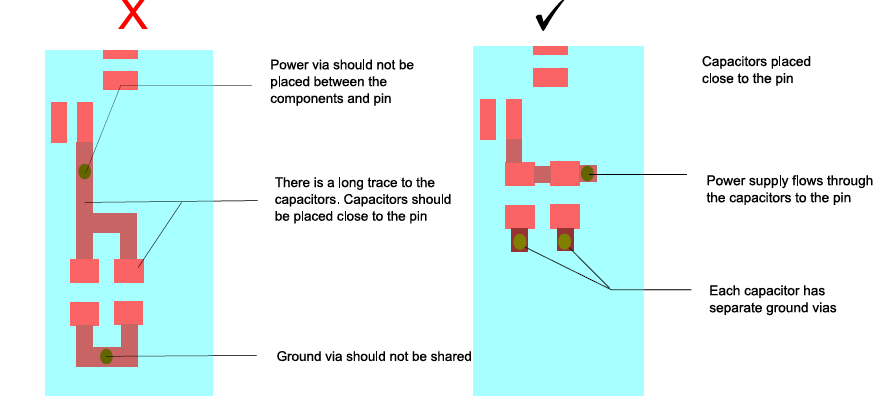
\includegraphics[width=0.7\textwidth]{Chap03/Figures/power_supply_coupling.PNG}
		\caption{Power Supply Decoupling}
		\label{fig:Power_Supply_Decoupling}
\end{figure}

%%%%%%%%%%%%%%%%%%%%%%%%%%%%%%%%%%%%%%%%%%%%%%%%%%%%%%%%%%%%%%%%%%%%%%%%%%%%%%%%%%%%%%%%%%%%%%%%%%%%%%

\subsubsection{BluEnergy-355MC RF Matching Circuit Layout:}
It is always a good approach to have the matching circuit as tight as possible you can refer to the Figure\ref{fig:Antenna_matching_network} the matching circuit is placed as close as possible, to avoid any additional track length to create some extra RF stub effects.  Don't ever run any of the signal lines across the RF feed line and always make sure to place the IC and RF in the same direction this approach will avoid any strange track shapes which can cause parasitics. It is a good way to make sure the RF feed line to the antenna through the IC has the same width across the track length this will avoid any unnecessary filtering effect. The figure refers to all of above-mentioned RF layout design hints.
Figure\ref{fig:Antenna_matching_network} shows that matching components are tightly packed, and no signals run across the RF feed.

\begin{figure}[h]
	\centering
	\subfigure[Matching Network Layout]{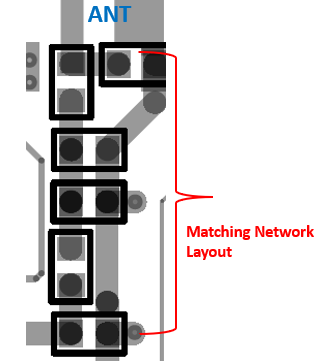
\includegraphics[scale=.8]{Chap03/Figures/matching_network_layout.PNG}}
	\qquad
	\subfigure[Matching Network Schematic]{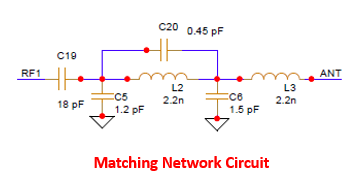
\includegraphics[scale=.8]{Chap03/Figures/matching_network_circuit.PNG}}
	\caption{BLE Antenna Matching Network}
	\centering
	\label{fig:Antenna_matching_network}
\end{figure}
We can place the components even overruling the component outline. Until we do not make the pads overlap, to achieve this we might have to bypass some PCB DRCs.

\subsection{Summary of the RF layout Design guidelines :}
\begin{enumerate}
	\item Keep Ground clearance as much as possible around the antenna.
	\item Make equi clearance on both sides of the antenna and RF feed line.
	\item Do not make a strange shape of the antenna feed line.
	\item Do not run any of the signal lines under the antenna or RF feed line.
	\item Make more vias from the top layer to the bottom layer for pure ground.
	\item Keep capacitive filters as near as possible to the power supply pins.
	\item Pack antenna matching network as close to antenna and IC RF feed.
	\item Place antennae in less clumsy are from other circuitry on the PCB.
	\item Make less overlap of the ground plane and power plane.
	\item Avoid high-frequency circuits around the RF feed.
	\item Always places the antenna at the edge of the PCB.
	\item Always chooses a standard pattern for the ground around the antenna.
	\item Never places any components, screws, mounting holes, or planes in the keep-out area of the antenna.
	\item The antenna must house with a Metalic shield to avoid external interference.
	\item There should not be direct ground under the antenna.
	\item The Orientation of the antenna should be inlined with the final PCB.
	\item When using the passive matching circuit try to have multiple components matching this can help at the debugging stage to tune the matching circuit.
\end{enumerate}



\section{Conclusion of the Chapter \ref{chap:BLE}}
The simulation and design of both the MIFA and IFA antennas are successful the results have been presented in Chapter\ref{chap:BLE}.  
Both the MIFa and IFa antennas are well performed in the sense of the results and design, because of the industry standards and Bluetooth stack recommendations, from vendors I have opted MIFA for Inventvm Bluetooth modules. 
The Layout is also quite impressive considering all norms of RF PCB layout guidelines, which are mentioned in the chapter\ref{chap:BLE}.
In the chapter\ref{chap:BLE} I have not stressed the theoretical calculation for the MIFA/IFA antenna because the calculations are pretty much the same as the standard MIFA and IFA antennas, 
The goal is to bring up the sophisticated RF BLE layout according to the application with a standard approach. Yet reference papers [\cite{MIFA_Design_Losito},\cite{MIFA_IFA_difference_Kanan}] give more insight into the theocratical design of the MIFA / IFA antenna and 
I have taken fewer opportunities to explain the nordic architecture, because of the RF layout out-wise and in the antenna sense, I have followed the same guidelines as I did for the BLUeNRG-355mc.
The Complete layout of the BLUeNRG and Nordic is attached in the chapter\ref{chap:miselleneous} , Figures (\ref{fig:BLUeNRG-355mc_BLE_Layout},\ref{fig:Nordic_nrf52840_BLE_Layout}).
\thispagestyle{empty}
\cleardoublepage
% % % % % % % % % % % % % % % % % % % % % % % % % % %
% % % % % % % % % % % % % % % % % % % % % % % % % % %
\chapter{Architecture of Wireless Communication Active Balancing BMS}\label{ch:Architecture_Active_Balancing_BMS}
\section{Introduction}
There are plenty of topologies dedicated to the BMS active balancing, for instance, cell-to-cell charge balancing, cell-to-stack or stack-to-cell charge sharing, and stack charge sharing. Among such wide techniques cell to stack and stack-cell, charge-sharing techniques gain the upper hand because of their robustness and safety measures against the battery.
\section{Active Balancing Topologies for BMS }

\subsection{\textit{Type Ia} : Combination of Buck and Boost Converter}

\subsection{\textit{Type Ia} : Combination of the Buck/Boost Converter :}
The figure\ref{fig:Type 1a Active Battery Balancing} illustrates the Type Ia balancing method for a battery system with n series-connected cells. The description is stack-to-cells-to-stack in accordance with the accepted nomenclature. A buck converter serves as a charging unit that distributes charge from the stack to the chosen cells. A boost converter reverses the process of discharge.
\\
The boost converter's input and output voltage ranges must be large enough to accommodate cells with voltages ranging from 1 to n-1. All cells can be actively charged and discharged up to the top level of the stack in this manner. It is only possible for nearby cells to balance numerous cells at once. Access to all cells below the topmost cell is used to balance that cell.
\\
This section explains the balancing procedure shown in Figure \ref{fig:Type 1a Active Battery Balancing}. The buck converter feeds Cell 1 with energy from the stack through switch \textit{$S_wA1$}. The converter output current $I_{Buck}$ is used to charge Cell 1. With the converter input current boost, the boost converter simultaneously discharges Cell 1 and Cell 2 through \textit{$S_wB2$}. The sum of the current in Cell 1 is 0A since $I_{Buck} = -I_{Boost} = I_{Bal}$, while Cell 2 discharges with $I_{boost}$A (negative balancing or "discharge mode"). The buck converter is often connected higher than the boost converter Batteries in Charging Mode. Discharging is done in the opposite order.
\\

\begin{figure}[h]
	\centering
	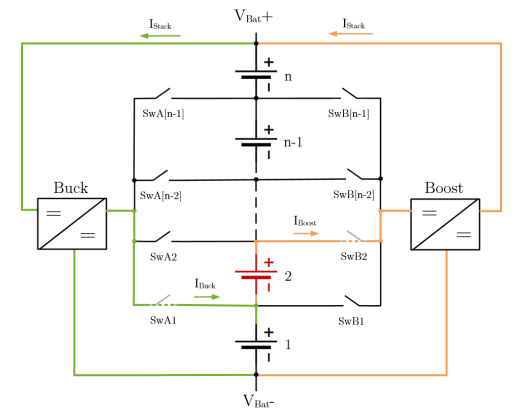
\includegraphics[width=0.7\textwidth]{Chap04/Figures/Type1a_ABMS.PNG}
	\caption{\textit{Type Ia}: Active Battery Balancing} 
	\label{fig:Type 1a Active Battery Balancing}
\end{figure}

The idle cell currents can be expressed as a vector following \ref{eq:Type1_cell_current}. It accounts for the balancing currents, both positive and negative, as well as the resulting stack current.
\begin{equation}\label{eq:Type1_cell_current}
    \vec{I_{Cell}}  = I_{stack} + \vec{I_n}\centerdot I_{Bal} - \vec{OUT}\centerdot I_{Bal}
\end{equation}

\begin{equation}\label{eq:Type1_cell_current}
    I_{stack}  = I_{Bal}(\frac{1}{\eta } \sum_{}^{}\vec{I_n}  - \eta\sum \vec{Out} ) \\
\end{equation}

\begin{equation}
\vec{OUT}  = \begin{pmatrix}
    S_{B1}\\
    \vdots
    S_{B[n-1]}  
\end{pmatrix} \\
, S_{x}=\left\{0\cdots1\right\}\\
, \vec{I_n}  = \begin{pmatrix}
    S_{A1}\\
    \vdots
    S_{A[n-1]}
\end{pmatrix} \\
\end{equation}

where $\vec{I_n}$ and $\vec{OUT}$ are the vectors of the switch signals $S_{A[x]}$ and $S_{B[x]}$ , respectively.
\\
The converter power and overall losses depend on the stack's n cells and the location of the balanced cell inside it. They rise as the position and the number of cells increases. \textit{I = J} when a single cell is in balance, In the absence of that, \textit{I} stands for the bottom cell of the balancing group and \textit{j} for the top one. As a result, \textit{I} and \textit{j} is always true.
\\
The necessary converters can be the traditional buck and boost converters depicted in Figures \ref{fig:Conventional Buck (a) and synchronous Buck(b) Conveter} and \ref{fig:Conventional Boost (a) and synchronous Boost(b) Conveter}. A synchronous design can be adopted, in which the diode is replaced with an actively regulated MOSFET to eliminate losses and to improve the efficiency of the converters across the whole operating range.
\begin{figure}[h]
	\centering
	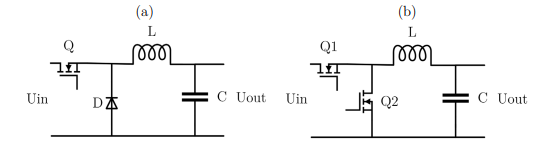
\includegraphics[width=0.9\textwidth]{Chap04/Figures/Conventiaonal_buck_synch_buck.PNG}
	\caption{Conventional Buck (a) and synchronous Buck(b) Conveter} 
	\label{fig:Conventional Buck (a) and synchronous Buck(b) Conveter}
\end{figure}

\begin{figure}[h]
	\centering
	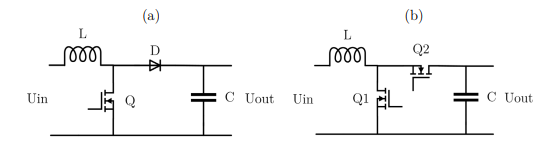
\includegraphics[width=0.9\textwidth]{Chap04/Figures/Conventiaonal_boost_synch_boost.PNG}
	\caption{Conventional Boost (a) and synchronous Boost(b) Conveter} 
	\label{fig:Conventional Boost (a) and synchronous Boost(b) Conveter}
\end{figure}

\subsection{\textit{Type Ib} : \textit{Type Ia} with a bidirectional converter :}
In terms of balancing routes, \textit{Type Ib} is comparable to \textit{Type Ia}. Bidirectional converters are used in place of unidirectional ones. Figure \ref{fig:Type1b Active Balancing Circuit } depicts the schematic for potential hardware implementation.\\

\subsection{\textit{Type IIa} :  Buck-boost converter :}
The Type IIa of the discussed balancing techniques is shown in Figure 50. Once more, n cells are arranged in series to make up the battery system. The description is cells-to-cells following the accepted nomenclature. This approach is comparable to cell bypassing if the load current and balancing current are the same. In discharge mode, a buck converter moves charge from one cell or many neighboring cells to its subjacent cells in the stack. A boost converter transfers charge in the other direction when it is in charge mode. A single bidirectional buck-boost converter can be created by combining the two converters.
\begin{figure}[h]
	\centering
	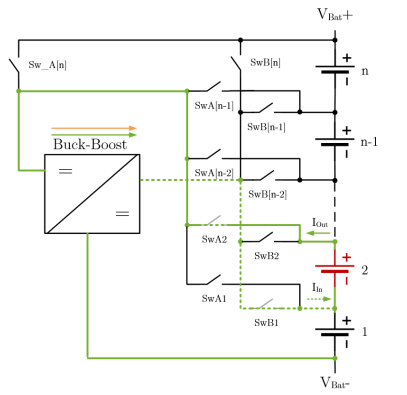
\includegraphics[width=0.6\textwidth]{Chap04/Figures/Type2a_ABMS.PNG}
	\caption{\textit{Type IIa} :  Buck-boost converter }
	\label{fig:Type2a Buck-boost converter}
\end{figure}
A bidirectional buck-boost converter made up of both converters is possible. To support 1 to n cells, the buck-boost converter's input and output voltage ranges must be sufficiently broad. Only cells that are close to one another can balance numerous cells at once. 
\\
\indent The explanation for the balancing procedure shown in Figure \ref{fig:Type2a Buck-boost converter} is given in the paragraphs that follow. Switches $S_{wA[2]}$ and $S_{wB[1]}$ in the buck converter allow the energy from Cells 1 and 2 to be transferred to Cell 1. 
it releases cells 1 and 2. The converter output current $I_{In}$ charges cell number one. In turn, Cell 1 is charged with $(I_{In} - I_{Out})$ A while Cell 2 is discharged with $I_{Out}$ A (negative balancing). $I_{Out}$ becomes $I_{Bal}$. 
In most cases, charging occurs when the DC/DC converter is connected in parallel to the desired cells and is in boost mode. However, in buck mode, discharge is performed in the same manner. Same charge and discharge operations as with \textit{Type I} are possible through switches $S_{wA[n]}$ and $S_{wB[n]}$.
\\
Depending on the number of balanced cells, the resulting cell current can be expressed as a vector:
\begin{equation}\label{eq:Type2_cell_current}
    \vec{I_{Cell}}  = \vec{I_{n}} \centerdot I_{Bal}  + \eta \centerdot \frac{\sum \vec{I_{n}}}{\sum \vec{I_{Out}}}\centerdot \vec{I_{Out}} \centerdot I_{Bal}
\end{equation}
\begin{equation}
    \vec{OUT}  = \begin{pmatrix}
        S_{B1}\\
        \vdots
        S_{Bn}  
    \end{pmatrix} \\
    , S_{x}=\left\{0\cdots1\right\}\\
    , \vec{I_n}  = \begin{pmatrix}
        S_{A1}\\
        \vdots
        S_{An}
    \end{pmatrix} \\
\end{equation}

\begin{figure}[h]
	\centering
	\subfigure[Conventional Buck-Boost Converter]{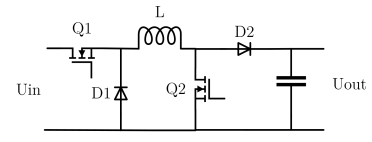
\includegraphics[scale=.7]{Chap04/Figures/Buck_boost_conventional.PNG}}
	\qquad
	\subfigure[Synchronous Buck-Boost Converter]{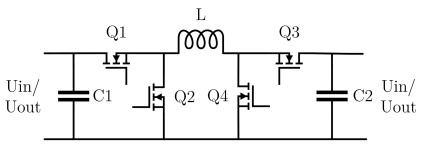
\includegraphics[scale=.7]{Chap04/Figures/Synchronous_buck_boost.PNG}}
	\caption{Typical Buck-Boost Converters}
	\label{fig:Type2a Typical Buck boost}
\end{figure}
Figure \ref{fig:Type2a Typical Buck boost}(a) depicts a potential buck-boost converter implementation. The N-MOSFET Q2 is disabled for buck mode, and Q1 is turned on and off. Q1 is constantly on in boost mode while Q2 is actively switched. The four-switch buck-boost converter from Figure \ref{fig:Type2a Typical Buck boost}(b)  may be used instead to enable synchronous mode.

\subsection{\textit{Type IIb} :  Bidirectional buck-boost converter :}
In terms of balancing routes, \textit{Type IIb} is comparable to \textit{Type IIa}. A bidirectional buck-boost converter is employed instead of a traditional (unidirectional) one. Because not every cell level requires a connection to both input and output, the number of MOSFETs needed in the switch-matrix is decreased. The same equations and exact operations are true for \textit{Type IIa} as well. Figure \ref{fig: Type2b active balancing architecture} displays the diagram and the power paths\cite{Active_Balancing_Thesis_Raber}[p. 60].
\begin{figure}[h]
	\centering
	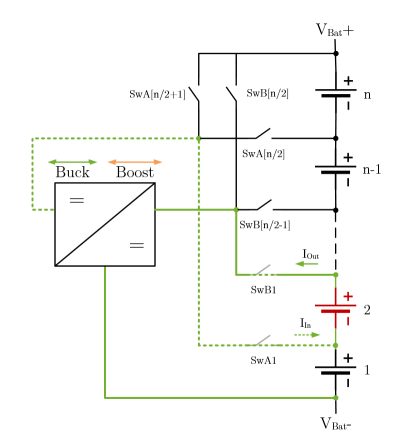
\includegraphics[width=.6\textwidth]{Chap04/Figures/Type2abABMS.PNG}
	\caption{\textit{Type IIb} active balancing architecture }
	\label{fig: Type2b active balancing architecture}
\end{figure}
A four-switch buck-boost converter similar to the one in Figure\ref{fig:Type2a Typical Buck boost}(b) can be used to realize the necessary bidirectional buck-boost converter. The ability to run the converter in a synchronous mode in both directions is a benefit of this design.


\subsection{\textit{Type IIIa} :  High - and low-side buck-boost converters :}
The system's implementation using high- and low-side buck-boost converters are shown in Figure \ref{fig:Type3a active balancing architecture}. Similar to \textit{Type I}, the operation involves the transfer of charge sequentially rather than simultaneously. There are two phases to the balancing process: one for the boost operation and one for the buck operation. The description is stack-to-cells-to-stack following accepted nomenclature. The high-side converter and low-side converter shouldn't work in the same direction at the same time to maintain a low average stack current throughout the two phases. To demonstrate how the high-side converter works in this example, balancing routes for \textit{Cell [n-1]} are also given in addition to \textit{Cell 2}\cite{Active_Balancing_Thesis_Raber}[p. 62].
Four converters, which can carry out the two phases concurrently, are used in an expanded version of this architecture\cite{Active_Balancing_Thesis_Raber}. There are more conceivable combinations: Another high-performance variant can be created by fusing the Type II concept with the Type III high-side converter.\\

\begin{figure}[h]
	\centering
	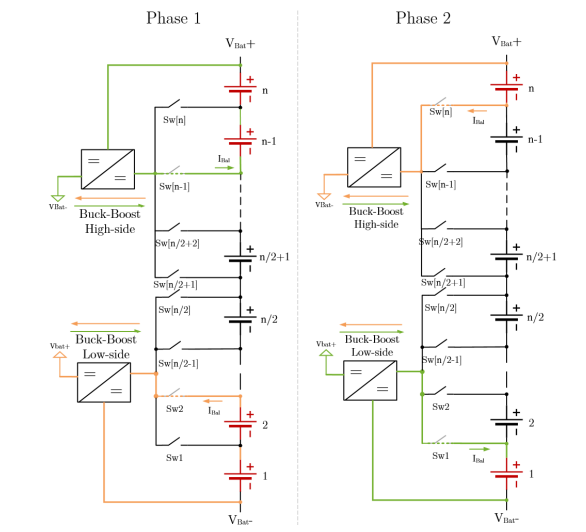
\includegraphics[width=0.6\textwidth]{Chap04/Figures/Type3a_ABMS.PNG}
	\caption{\textit{Type IIIa}  active balancing architecture}
	\label{fig:Type3a active balancing architecture}
\end{figure}
During Phase 1, the low-side converter functions as a boost converter, discharging \textit{Cells 1} and 2 through $S_{wA}$ with the converter's input current IBal, identical to Example \ref{fig:Type3a active balancing architecture}. \textit{Cell [n-1]} and \textit{Cell [n]} are simultaneously charged with IBal by the high-side converter while operating in buck mode. Phase 2 involves charging Cell 1 in buck mode and discharging \textit{Cell [n]} in boost mode to achieve the same balancing results as in Section (Results will be published in the upcoming chapters ). $I_{Bal}$ is used to charge and discharge \textit{Cell [n-1]} and \textit{Cell 2}.\\
A common ground connection allows the low-side converter to access all cells up to the middle of the battery stack, including \textit{Cell [n/2]}. It can be executed as depicted in Figure \ref{fig:Typical Schematics of the Low side and High Side buck boost Converter}. The design is made simpler by the fact that the two operating modes are only required in one direction. To enable synchronous operation for both modes, only two MOSFETs are required. If switch Q1 is not controlled, the MOSFET's intrinsic antiparallel diode enables normal operation albeit with lower efficiency.\\
The remaining cells are connected to the high-side converter through a shared $V_{Bat+}$ link. It is similar to the common ground converter in terms of design, but it has a distinct structure (see Figure \ref{fig:Type3a active balancing architecture}).
\section{Proposed Active Balancing Method}
The proposed architecture for the BMS active balancing is very similar to the \textit{type IIa and IIb} active balancing. In the proposed topologies the charge is transferred either from imbalance cell to stack or vice versa.
A bidirectional high and low-side buck-boost converter is used in the proposed architecture in place of the typical (unidirectional) buck-boost converter. Refer\ref{fig:BMS Architecture} to the Architecture to see how the switch matrix is set up to connect each battery node to the DC/DC converter's low side. The top of the battery pack is directly attached to the high side of the DC/DC converter.
\begin{figure}[h]
	\centering
	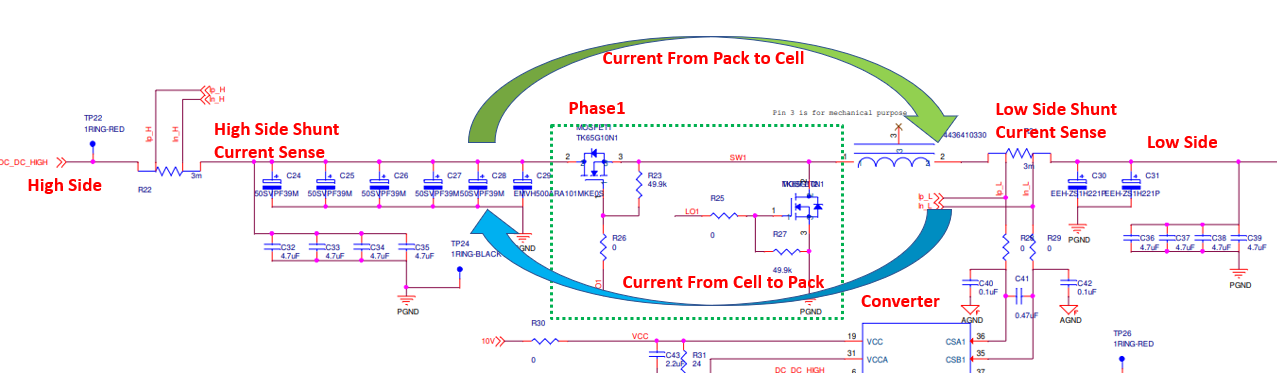
\includegraphics[width=1\textwidth]{Chap04/Figures/Low_high_side_Converter_shematic.PNG}
	\caption{Shematic of the High/Low side DC/DC converter } 
	\label{fig:High_Low_DC_DC_Shematic}
\end{figure}
The proposed architecture\ref{fig:High_Low_DC_DC_Shematic} gives more control over the balancing current that is flowing in the DC/DC controller. One of the acute advantages of the input(With High side shunt Resistance) and output current(With Low side shunt Resistance) to the DC/DC converter. The section gives a more elaborative description and technical details of this configuration.
\section{Overview of Active balancing BMS Architecture}
Figure\ref{fig:BMS Architecture} shows the overview of the Inventvm wireless BMS architecture. From the Hardware point of view, the Architecture is separated into two parts one Cell Management Unit (CMU) which sits on each battery. The other one is MMU which is on the main motherboard to control the overall functionality of the BMS. The working procedure of the architecture is as follows
\begin{figure}[h]
	\centering
	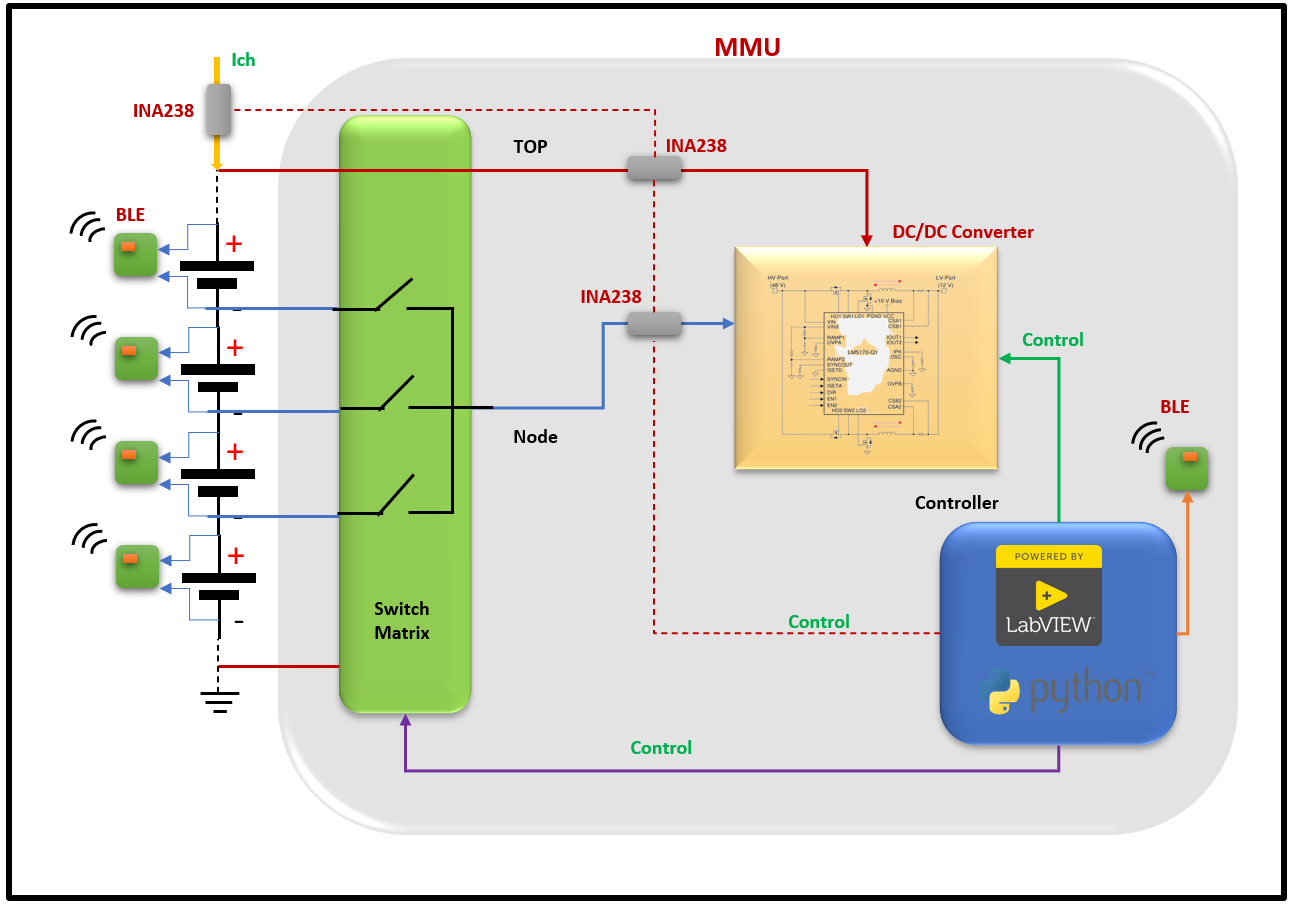
\includegraphics[width=1\textwidth]{Chap04/Figures/BMS_Architecture_border.PNG}
	\caption{BMS Architecture} 
	\label{fig:BMS Architecture}
\end{figure}
\begin{itemize}
	\item The CMUs of each battery contains Bluetooth modules, for our applications we have used BLUeNRG-355mc which will sense the live battery voltage and the temperature of the battery(using NTC).
	\item CMUs will synchronize with the master present on the MMU. According to the master request, all the CMUs Bluetooth will send the data to the Master in the given time slot.
	\item On request of the controller, the master(BLE on MMU) will collect packets from all the slaves(CMUs) and hand over the decoded data (Voltages of the Batteries and Temperature measurements) to the Controller on the MMU.
	\item The controller in this project is the PC, it could be a microcontroller also. The controller will be responsible for running all the BMS algorithms and detecting which node needs to be balanced depending on the CMU's battery voltages.
	\item In this particular project, the controller will use LabVIEW and python to build a complete BMS model and algorithm.
	\item Through the open circuit voltage(Battery voltages) received from the CMU, the controller will calculate the initial SoC(The open circuit voltage directly proportional initial SoC of the battery "manufacturer open circuit voltage to SoC curve").
	\item Once the controller finds the imbalance node through the initial SoC estimation from the open circuit voltages of the battery, the switch matrix is switched to the imbalance node and directly connected to the low side(Output) of the DC/DC converter.
	\item Depending on the battery imbalance the controller will configure the DC/DC converter either in buck or boost mode.
	\item During the Balancing, the input and output current of the DC/DC is monitored to calculate the balancing current, if the balancing current reached the threshold the DC/DC converter current is dropped.
	\item If the batteries are charging during the balancing the charging current \textit{$I_{ch}$}(Figure \ref{fig:BMS Architecture}) is also monitored through the pack current sensor.
\end{itemize}
\section{Retrospect of BMS Hardware}
\subsection{Multiphase Bidirectional DC/DC Current Controller LM5170-Q1}
\indent The LM5170-q1\cite{TI_LM5170_User_Datasheet} controller is a high precision dual phase bidirectional converter applicated in automotive 48 Volts and 12Volts dual battery systems.
Depending on the Direction Signal DC/DC converter regulates the average current. 
The Regulated current through the DC/DC converter can be programmed by analog or Digital PWM inputs.

The LM5170-q1\cite{TI_LM5170_User_Datasheet} has a dedicated dual phase differential current sense amplifier to monitor the current flowing through the Dc/Dc converter, which can achieve $1\%$ current sense accuracy.
It has a Robust Gate driver to drive half the bridge. The Internal gate driver of the LM5170 has the capability of driving parallel MOSFET switches with a capacity of 500Watts. 
The synchronous diode emulation mode prevents the dc to dc converter from the negative currents and also enables the discontinuous mode of operation. This property enhances the DC/DC converter efficiency tremendously. The Controller can offer benefits of cycle-by-cycle current limitation, overVoltage protection at both low side and high side ports, Temperature protection and Mosfet failure so on...
\\
\indent An innovative average current mode control scheme maintains constant loop gain, allowing a single R-C network
to compensate both buck and boost conversion\cite[p .2]{TI_LM5170_User_Datasheet},\cite{TI_LM5170_EVM_User_Guide}. The oscillator is adjustable up to 500 kHz and can synchronize
to an external clock. Multiphase parallel operation is achieved by connecting two LM5170 controllers for 3-
or 4-phase operation, or by synchronizing multiple controllers to phase-shifted clocks for a higher number of
phases. A low state on the UVLO pin disables the LM5170 in a low current shutdown mode\cite{TI_LM5170_User_Datasheet}.

\subsubsection{Definition of IC LM5170 Operation Modes:}
\begin{itemize}
    \item \textbf{Shutdown Mode:} When the UVLO pin is < 1.25 V, VCC < 8 V, or default < 1.25 V, the LM5170 is in
    shutdown mode with all gate drivers in the low state, all internal logic reset, and the VINX pin disconnected
    from the VIN pin. When UVLO < 1.25 V, the IC draws < 20 µA through the VIN and VCC pins\cite{TI_LM5170_User_Datasheet}.
    \item \textbf{Initialization Mode:}  When the UVLO pin is > 1.5 V but < 2.5 V, VCC > 8.5 V, and nFAULT > 2 V, the LM5170
    establishes proper internal logic states and prepares for circuit operation\cite{TI_LM5170_User_Datasheet}.
    \item \textbf{Standby Mode:}  When the UVLO pin is > 2.5 V, VCC > 8.5 V, and nFAULT > 2 V, the LM5170 first
    performs fault detection for 2 to 3 ms. During this time, the external power MOSFETs are each checked for
    drain-to-source short-circuit conditions. If a fault is detected, the LM5170 returns to shutdown mode and is
    latched in shutdown until reset through the UVLO or VCC pins. If no failure is detected, the LM5170 is ready
    to operate. The circuit breaker MOSFETs are turned on and the oscillator and ramp generators are activated,
    but the four gate drive outputs remain off until the EN1 or EN2 initiate the power delivery mode\cite{TI_LM5170_User_Datasheet}.
    \item \textbf{Power Delivery Mode:}  When the UVLO pin > 2.5 V, VCC > 8.5 V, nFAULT > 2 V, EN1 or EN2 > 2 V, DIR
    is valid (> 2 V or < 1 V), and ISETA > 0 V, the SS capacitor is released and the LM5170 regulates the DC
    current at the level set at the ISETA pin\cite{TI_LM5170_User_Datasheet}.
\end{itemize}

\subsubsection{Bench setup and operation of the DC/DC Converter :}
Although LM5170 can perform full bridge operation, we need only the half-bridge with a full current rating for our application. Figure\ref{fig:LM5170_DC_DC_Converter_Operation_Setup} only the high side bridge is used for buck and boost operations. The Figure shows the typical setup to operate the DC/DC converter in the bidirectional power system environment. The combination of the Load on the High side is the Battery pack Top and on the Low side, the is Battery pack node.  A current Can flow from the High side to the low side or vice versa depending on the direction. The direction of the current flow depends on the BMS algorithm. A BMS algorithm decides which no needs to be balanced depending on batteries voltage difference. 
\begin{figure}[h]
	\centering
	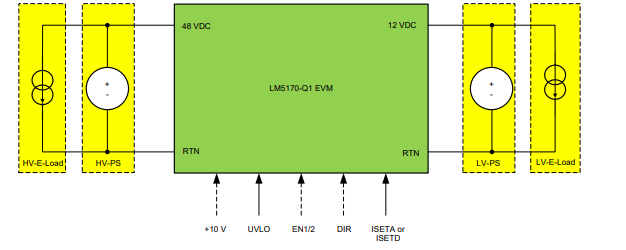
\includegraphics[width=1\textwidth]{Chap04/Figures/DC_DC_Converter_bench_setup.PNG}
	\caption{LM5170 DC/DC Converter Operation Setup \cite{TI_LM5170_BatteryTesting_Solution},\cite{TI_LM5170_EVM_User_Guide} }
	\label{fig:LM5170_DC_DC_Converter_Operation_Setup}
\end{figure}

\subsubsection{The operation of the DC converter is as follows (The Figure \ref{fig:LM5170_DC_DC_Converter_Operation_Setup}) :}
\begin{itemize}
    \item Connect the High side and Low side Battery pack nodes (Low or High side could be electronics loads also).
    \item Apply a voltage > 2.5 V and < 6 V  to the UVLO pin to release it from the shutdown mode.
    \item Select the EN1 or EN2 to enable the dc to dc converter output, for instance, EN1 is the output enable signal for phase1 and EN2 is the output enable signal for phase 2.
    \item Depending on the mode of operation Apply DIR pin voltages. Direction command input. Pulling DIR above 2 V sets the converter to buck mode, which commands the current to flow from the HV-Port to LV-Port. Pulling DIR below 1 V sets the converter to boost mode, which commands the current to flow from the LV-Port to HV-Port. If the DIR pin is left open, the LM5170 detects an invalid command and disables both phases with the MOSFET gate drivers in the low state\cite[p .5]{TI_LM5170_EVM_User_Guide}. 
    \item Use the ISETA signal to set the current.ISETA is the analog current programming pin. The inductor DC is proportional to the ISETA voltage. Use either ISETA or ISETD but not both for phase current programming. When ISETA is not used, connect a 100-pF to 0.1-µF capacitor from ISETA to AGND\cite[p .5]{TI_LM5170_EVM_User_Guide}.
    \item If the ISETD is used, The PWM current programming pin. The inductor DC level is proportional to the PWM duty cycle. Use either ISETA or ISETD but not both for phase current programming. When ISETD is not used, short ISETD to AGND \cite[p .6]{TI_LM5170_EVM_User_Guide}.
\end{itemize}
\subsubsection{Summary of the DC/DC Converter:}
\indent Although DC/DC Converter LM5170 is capable to use the dual phases, we have limited the DC/DC converter to the single phase according to the Type ii BMS DC/DC converter configuration. Depending on the user's need user can use ISETA or ISETD to setting the current flowing in the dc to dc converter. For Instance, if the user uses a microcontroller it is much more convenient to use the PWM, so the ISETD is a natural choice, If the user opts Central pc/ Labview application it is much better to use ISETA through some analog supply. Ultimately ISETD (PWM) converted to the Analog voltage to set the current.
\subsection{Switch Matrix :}
Automotive BMS applications demand sophisticated and robust switch matrices, as in the market there are no switch matrix will available according to the application. There has been specific knowledge used to pick this switching component. Switching components are more unlikely than the conventional components, such a vote for picking the switching components always registered for the high power MOSFETs because of various technological advantages over conventional electro-mechanical switches. Since the component choice is entirely left to the design engineer, it is always a good practice to design these switch matrix boards from scratch to have full control over the system. The following sections will give more insights into the switch matrix.
\begin{figure}[h]
	\centering
	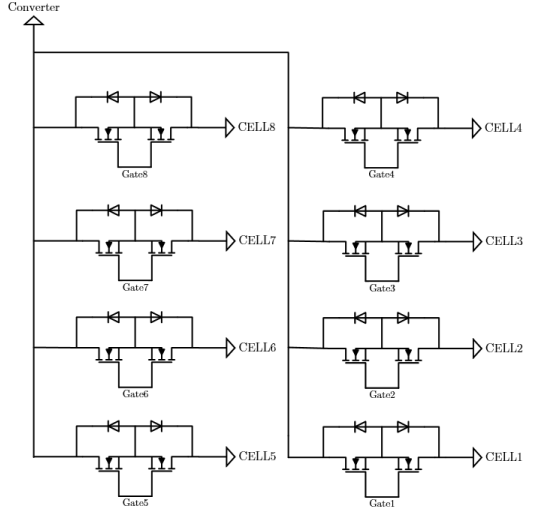
\includegraphics[width=0.8\textwidth]{Chap04/Figures/switch_matrix.PNG}
	\caption{Typical Mosfet switch matrix for 8 batteries \cite{Active_Balancing_Thesis_Raber} }
	\label{fig:Mosfet_Switch_Matrix}
\end{figure}
\indent Single or double back-to-back FETS are used for the switch matrix, back to back MOSFETS are two MOSFETs housed in a single package or externally by connecting the gates of FETs are common. The Figure\ref{fig:Mosfet_Switch_Matrix} implicates one such example of a switch matrix using the back-to-back MOSFETs.

\subsubsection{The initiative understanding behind choosing the switch matrix MOSFET:}
\begin{itemize}
    \item Low Rds ON; low on-state resistance implicates that MOSFET can carry high DC with lower dissipation.
    \item High Blocking voltage; High blocking voltage between the drain and the source ensures the breakdown safety of the MOSFET against the full Battery pack voltage.
    \item Low gate area - to drive the FET faster, and it cost less than the current budget for the FET's gate driver.
    \item Low gate drive voltage. So-and-so forth.
\end{itemize}

\noindent By analyzing the criteria mentioned in the section, the choice is made to use STD20NF06L for the switch matrix. The component specification is as follows :
STD20NF06\cite{Switch_MatrixFET_STD20NF06L} is the high-power MOSFET that has been developed for automotive applications to handle the High current with very low input gate capacitance. The FET has perfect dv/dt. STD20NF06 is DPACK package which is quite big compared to SMD package and single package dual back-to-back FET's, yet the FET is opted for because of the following benefits. The back-to-back FET arrangement is made externally as shown in Figure \ref{fig:Mosfet_Switch_Matrix}.
for more insights into the component refer to the MOSFET Datasheet \cite{Switch_MatrixFET_STD20NF06L}.
	


\begin{center}
\begin{tabular}{ |p{4cm}|p{4cm}|p{4cm}|p{4cm}|  }
\hline
\multicolumn{4}{|c|}{STD20NF06L Datasheet} \\
\hline
Symbol& Parameter &Value & Unit \\
\hline
$V_{ds}$  & Drain-source voltage & 60 & V \\
$V_{gs}$  & Gate-source voltage  & $\frac{+}{-}$ 18 & V \\
$I_{d}$   & Drain current (continuous) at $ TC = 25 \deg C$ & 24 & A \\
$P_{Tot}$ & Total power dissipation at $ TC = 25 \deg C$    & 60 & W \\
$\frac{dv}{dt}$ & Peak diode recovery voltage slope    & 10 & $V/ns$ \\
$C_{iss}$ & Input capacitance VDS = 25 V, f = 1 MHz, VGS = 0 V, & 660 & C \\
$R_{ds(on)}$ & Static drain-source on-resistanc & @VGS = 10V,@ID = 12A, 32  & $\Omega$ \\
\hline
\end{tabular}
\end{center}
\subsection{Matrix Switch Gate Driver :}
Modern BMS application is suffocated by the hot swapping of the Batteries for balancing. When the battery node is switched in the battery pack to balance the battery node matrix(switching circuit) the MMU will see an immense current that is flowing from the battery \cite{LTC4231_User_Datasheet}. when the switch matrix is switched to a particular node of the battery pack. The battery Node will be directly connected to the output node of the DC/DC converter (The low side of the DC/DC Converter refers to the circuit \ref{fig:Typical Bidirectional circuit of the LM5170} @low side), which will be having reservoir capacitor that will sink an immense amount of the current from the battery in very short time this will cause switching FET to burn, so it essential to switch FET very carefully. such technique is called "Hot Swap". "Hot Swap" is FET switching technique Figure\ref{fig:Mosfet_Switch_Matrix}, more often used in live power switch applications. The technique allows the gate driver circuit to monitor the current flowing through the switch circuit by the input sense resistance. By any chance Hot swap circuit doesn't allow the rapid surge of the load current in the switch circuit \cite{LTC4231_User_Datasheet}.
\subsubsection{LTC4231 :}
LTC4231 is an Analog Device Inc Micro power hot-swap controller that is employed to face circuit board insertion and abrupt live power supply. An internal high-side switch driver controls the gate of an external N-channel MOSFET. Back-to-back MOSFETs can be used for reverse supply protection down to –40V \cite{LTC4231_User_Datasheet}.

The LTC4231 provides a debounce delay and allows the GATE to be ramped up at an adjustable rate. After startup, the LTC4231's quiescent current drops to 4µA during normal operation with output active. UVL, UVH, OV, and GNDSW monitor overvoltage and Undervoltage periodically, keeping total quiescent current low. Pulling SHDN low shuts down the LTC4231 and the quiescent current drops to 0.3µA.

During an overcurrent fault, the LTC4231 actively limits current while running an adjustable timer \cite{LTC4231_User_Datasheet}. The LTC4231-1 remains off after a current fault while the LTC4231-2 automatically reapplies power after a cool-down period\cite{LTC4231_User_Datasheet}.

A typical circuit diagram and the operational waveforms of the LTC4231 are described in the Figure\ref{fig: LTC4231 Application circuit and the Operational waveform }. 
For more technical details refer to the ADI LTC4231 datasheet\cite{LTC4231_User_Datasheet}.

\subsubsection{Inrush Current Control by LTC4231 :}
In most, automotive applications keeping the inrush current low and in control is essential to avoid catastrophic damage to the switching circuits. LTC4231 takes a golden hand in controlling the inrush current by startup method (Timer Delay varying). The equations \ref{eq:LTC4321_Inrush_current} implicate the Inrush current controlled by the LTC, the Inrush current highly depends on the gate capacitance of the switch, and the output capacitance of the DC/DC capacitance (load Capacitance $C_L$). A capacitor $C_G$ of the Gate to the GND can be used to control the gate voltage slew rate for the Inrush current in the Switch.
\begin{equation}\label{eq:LTC4321_Inrush_current}
    I_{InRsush} = \frac{C_{L}}{C_{G}} \times 10\mu A
\end{equation}
\begin{figure}[h]
	\centering
	\makebox[\textwidth]{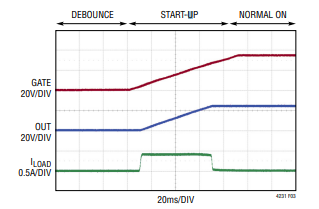
\includegraphics[width=0.4\paperwidth]{Chap04/Figures/Inrsuh_current_of_LTC4321.PNG}}
    \caption{Inrush Control by Limiting $V_{GATE}$ Slew}
    \label{fig: LTC4231 Inrush Control by Limiting Vgate Slew}
\end{figure}
The $V_{GATE}$ of the switch raise with the slope of $10\mu A/C_G$.
Once $V_{GATE}$ crosses the Vth, status goes high impedance. see the figure\ref{fig: LTC4231 Inrush Control by Limiting Vgate Slew} which explains the Inrush current protection when the $\Delta V_{Th(GATE)}$ crosses the gate voltage threshold.

The Design Example in the Chapter\ref{chap:miselleneous} explains, how to pick the design parameters to design the inrush current limit and gate driver, please follow. LTC4231 holds a wide range of advantages compared to the gate driver that is available in the market such Wide Operating Voltage Range: 2.7V to 36V, Reverse Supply Protection to –40V n Adjustable Analog Current Limit with Circuit Breaker n Automatic Retry or Latchoff on Current Fault n Overvoltage and Undervoltage Monitoring n Controls Single or Back-to-Back N-Channel MOSFETs \cite{LTC4231_User_Datasheet}. By considering all the facts we have picked the LTC4321 as the gate driver for the switch matrix.
\subsection{Current Sense :}

As elaborated in the BMS architecture High precision current sensors are used to monitor the BMS Currents. The currents are mainly monitored by the sensor charging current that is entering through the Battery pack Top and balancing current that is entering or leaving from the DC to Dc convert to the Balancing node from Battery pack TOP.

For Inventvm active balancing BMS application, The team has selected INA238 Current sensor from Texas instruments. Chapter \ref{ch:Current_Measurement} gives an extensive explanation for choosing the INA238\cite{INA238_User_Datasheet} and the application \ref{sec:INA238}.
\subsection{Wireless Communication Hardware :}
The Bed Rock Idea behind the Inventvm active balancing BMS is to make the BMS architecture in the Wireless Communication Environment. The wireless communication architecture will reduce the immense pain of hard wires for communication in modern smart EVs. The Wireless Communication picked for the project is the Bluetooth stack, Chapter \ref{chap:BLE} takes the privilege to explain the Bluetooth Hardware choosing criteria, and design the proprietary Bluetooth solution for the projects. The BLUeNRG-355MC\cite{BLNRG355_STEVAL_GUIDE} and the Nordic\cite{NORDIC_nrf52840_USERGUIDE} are the Bluetooth solutions employed in the project.
\section{Summary of Chapter \ref{ch:Architecture_Active_Balancing_BMS}}
The initial phase of the chapter \ref{ch:Architecture_Active_Balancing_BMS} summarizes the different topologies of the BMS active balancing, more or less, many of the topologies remained on the shelf, because of the less robustness and clumsy implementation.
The proposed topology\ref{fig:High_Low_DC_DC_Shematic} for the BMS active balancing is inherited from topology \textit{Type IIa} and topology \textit{Type IIb}. Currently, by using the proposed methodology\ref{fig:High_Low_DC_DC_Shematic}, we can successfully perform the active balancing for batteries.
The active balancing BMS architecture\ref{fig:BMS Architecture} will give a much broader view in this chapter \ref{ch:Architecture_Active_Balancing_BMS}, but in this architecture\ref{fig:BMS Architecture}, I have not discussed how to calculate the SoC and SoH but following Chapters(SoC and SoH calculation chapter not yet updated) will give more extravagance on the SoC and SoH calculation and synchronization methods of the voltage and current. I have succeeded in explaining most of the BMS hardware except the current sensors because I have dedicated a separate chapter to explaining the current acquisition and synchronization(Current and Voltage synchronization chapter not yet updated) of the measurements.
\thispagestyle{empty}
\cleardoublepage
% % % % % % % % % % % % % % % % % % % % % % % % % % %
% % % % % % % % % % % % % % % % % % % % % % % % % % %
\chapter{Current Measurement For SoC Estimation}\label{ch:Current_Measurement}
SoC is the most crucial parameter of the battery to estimate in the BMS. In the deal case, the SoC of the battery has to be measured continuously, well which is not feasible since we have a measuring setup (sensors ) we need to discretize the time and, measure how much current flows through the battery to estimate the soc. To be precise in the current measure to estimate battery soc we need to account for all currents that flow in and outwards from the battery. In the active balancing setup, we have a minimum of three currents that need to be synchronized to estimate the battery soc, DC/DC converter input and output currents, and battery pack charging and discharging current. In an integrated circuit solution current measuring is very easy by designing all the sensors operating with a master clock and reading by an internal bus. Since the project is at a discrete solution level we have several current sensors associated with reading the currents. The following sections elaborate on a competitive solution for current reading and its usage in the project.
\section{Current Sensing}
To address the difficulties of creating an accurate current-measurement circuit for cost-effective applications, designers have a variety of choices at their disposal. The best flexibility is provided by using general-purpose operational amplifiers (op amps) or analog-to-digital converters (ADCs), they could be standalone or embedded in a microcontroller (MCU). While also leveraging a wide range of tailored components that are specifically made for current sensing but also address challenges in a specific way \cite{TI_Current_Sensing}.
Shunt resistors(Kelvin method) and/or hall sensors are the two methods more widely used methods in automotive BMS applications to measure the battery pack current(Charging/Discharging and Balancing current). The integrated solutions for measuring current is more preferable, to secure the space and power constraints in automotive applications. The following sections will give more insights into the current sense methods.

\section{Hall Effect Current Sensors }
"The Hall effect is the creation of a voltage difference (the Hall voltage) across an electrical conductor that is transverse to an applied magnetic field perpendicular to the current and an electric current in the conductor". Well, that is a bit of a more scientific and deep mathematical explanation of the Hall effect. If I take a little leverage to explain the Hall effect in the nomenclature The Current flow in the conductor causes to induce magnetic flux inside the magnetic core, these fluxes also turn out a small potential, which can be called hall voltage. The Hall voltage dropped across the coil (Magnetic) is directionally proportional to the current flowing in the conductor.
A galvanically isolated Hall effect current sensor capable of DC or AC measurement with high accuracy, excellent linearity, and temperature stability\cite{TI_Hall_Current_Sensing_TMCS1107}.
Let us explore hall sensors with some typical examples in the BMS such as the TMCS1107xx \cite{TI_Hall_Current_Sensing_TMCS1107} series from the TI are the most popular and competitive galvanic solutions for measuring the current.

\subsection{TMCS1107xx Sensors :}
The TMCS1107-Q1 is a galvanically isolated Hall effect current sensor with high accuracy, great linearity, and temperature stability for measuring DC or AC currents. A signal chain with low drift and temperature compensation offers a $3\%$ full-scale error over the device temperature range.\\
A magnetic field is created by the input current flowing through an internal 1.8-m conductor, which is monitored by an integrated Hall-effect sensor. This topology reduces design complexity and does away with external concentrators. Reduced conductor resistance decreases thermal and power loss. A 420-V lifetime working voltage and a 3-kV RMS minimal isolation between the current path and circuitry are provided by inherent galvanic insulation. Transient immunity and high common-mode rejection are made possible by integrated electrical shielding. \\
The output voltage is proportional to the input current. Fixed sensitivity minimizes ratiometry errors and enhances supply noise rejection, enabling the TMCS1107-Q1 to run from a single 3-V to 5.5-V power supply. When current enters the positive input pin, it is regarded as having a positive polarity. There are options for both unidirectional and bidirectional sensing.\\
\begin{figure}[h]
	\centering
	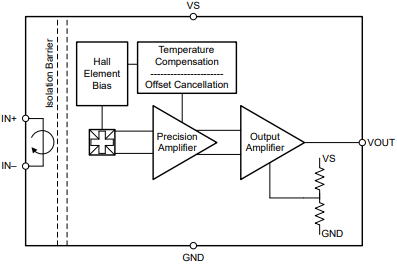
\includegraphics[width=0.6\textwidth]{Chap05/Figures/TMCS1107_HallSensor.PNG}
	\caption{TMCS1107xx Hall sensor Block diagram} 
	\label{fig:TMCS1107xx Hall sensor Block diagram}
\end{figure}
Input current to the TMCS1107-Q1 passes through the isolated side of the package lead frame through the
IN+ and IN– pins. The current flow through the package generates a magnetic field that is proportional to the
input current and measured by a galvanically isolated, precision, Hall sensor IC. As a result of the electrostatic
shielding on the Hall, sensor die, only the magnetic field generated by the input current is measured, thus limiting
input voltage switching pass-through to the circuitry\cite{TI_Hall_Current_Sensing_TMCS1107}.

\section{Shunt Resistors for Battery Current Measurement}
Sensing the voltage drop across a shunt or current-sense resistor \ref{fig:INA_high_side_currentsense} to determine the current in the most typical way. It is necessary to look at the parametric values of both the resistor and current-sense amplifier to obtain a very precise measurement of the current.
Accuracy loss must be prevented by carefully planning the connections between the current-sense amplifier and the resistor.
\begin{figure}[h]
	\centering
	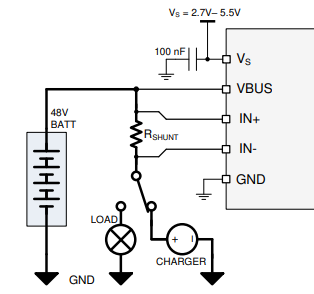
\includegraphics[width=0.4\textwidth]{Chap05/Figures/INA_high_side_currentsense.PNG}
	\caption{ INA238 High-Side Shunt Current Sensing} 
	\label{fig:INA_high_side_currentsense}
\end{figure}

INA2XX series shunt current sensors are the most competitive solution offered by TI to measure the high-side and low-side shunt current with high precision. INA238 is used in this project to measure the shunt current, bus voltage, and several other parameters. Section \ref{sec:INA238} will talk extensively about the INA238 and the features offered by the sensor to synchronize current measurements for BMS application.
\section{INA238/INA2xx}\label{sec:INA238}
The INA238 is a 16-bit delta-sigma ADC with an ultra-precise digital power monitor that is made primarily for current-sensing applications. With a common-mode voltage support range of -0.3 V to +85 V, the device can measure a full-scale differential input of $\pm$163.84 mV or $\pm$40.96 mV via a resistive shunt sensing element.
The INA238 does the necessary calculations in the background while reporting current, bus voltage, temperature, and power. The embedded temperature sensor is useful for tracking the system's ambient temperature and has a die temperature measurement accuracy of 1°C.

The INA238 can be utilized in accurate systems without undergoing multi-temperature calibration during production thanks to its low offset and gain drift design. Additionally, a wide dynamic range is provided without considerable power dissipation losses on the sensing shunt element thanks to the extremely low offset voltage and noise. This enables use in A to kA sensing applications. Due to the device's low input bias current, bigger current-sense resistors can be used, resulting in precise current readings in the micro-amp range.
The device supports samples averaging from 1x to 1024x and adjustable ADC conversion durations from 50$\mu$ s to 4.12 ms, which further reduces noise in the measured data.

\begin{figure}[h]
	\centering
	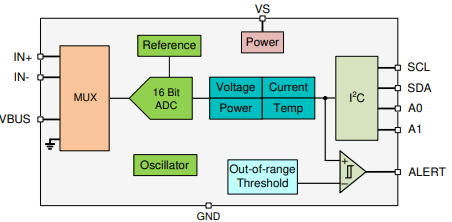
\includegraphics[width=0.6\textwidth]{Chap05/Figures/INA238_Simplified_Block_diagram.PNG}
	\label{fig:INA238_Simplified_Block_diagram}
	\caption{INA238 Simplified Block diagram \cite{INA238_User_Datasheet}}
\end{figure}

The INA238 has a multifunctional, open-drain ALERT output pin that can be utilized to report various problems or as a sign that the ADC conversion is finished while the device is functioning in both triggered and continuous conversion mode. Every time an output value under continuous monitoring exceeds its corresponding out-of-range threshold, the diagnostics mentioned in Table 7 in the user datasheet of INA238 \cite{INA238_User_Datasheet}  can be transmitted via the ALERT pin.

% \begin{table}[h]
%     \centering
%     \begin{tabular}{|l|l|l|}
%     \hline
% 		INA238 DIAGNOSTIC & STATUS BIT ALRT REGISTER (RO) & OUT-OF-RANGE THRESHOLD REGISTER (R/W)  \\ \hline
%         Shunt Under Voltage Limit & SHNTUL & SUVL\\ \hline
%         Shunt Over Voltage Limit & SHNTOL & SOVL \\ \hline
%         Bus Voltage Over-Limit & BUSOL & BOVL \\ \hline
%         Bus Voltage Under-Limit & BUSUL & BUVL \\ \hline
%         Temperature Over-Limit & TMPOL & TEMP\_LIMIT \\ \hline
%         Power Over-Limit & POL & PWR\_LIMIT & 0x7FFF H \\ \hline
%     \end{tabular}
% \end{table}

The diagnosis that prompted the ALERT pin can be identified by reading the DIAG ALRT register. In addition to configuring some ALERT pin functions, this register, which is depicted in Table 7 (user datasheet of INA238 \cite{INA238_User_Datasheet}), is also utilized to monitor other related diagnostics.

\begin{itemize}
	\item Alert latch enables — In the event that the ALERT pin is activated, this feature will maintain the pin's value even after all diagnostic circumstances have been resolved. The status of the ALERT pin is reset by reading the DIAG ALRT register. By setting the ALATCH bit, this function is made available.
	\item Conversion ready enable —  When an ADC conversion is finished and the output values are prepared to be received through the digital interface, the CONVERTION READY ENABLE signal instructs the ALERT pin to assert. Setting the CNVR bit enables this feature. Regardless of the CNVR bit set, the conversion completed events can also be read through the CNVRF bit.
	\item Alert comparison on averaged output — Enables comparison of the out-of-range threshold value to the ADC's averaged data values. Comparing the output data to the out-of-range threshold, this aids in further removing noise from the data to prevent false alarms brought on by noise. However, because of the time required for averaging, the diagnosis will be postponed. Setting the SLOWALERT bit activates this feature.
	\item Alert polarity — Allows the device to flip the ALERT pin's active state. Keep in mind that the ALERT pin is an open-drain output that requires a resistor to be pulled up. The APOL control bit can be used to change the ALERT pin's default active-low function to an active-high one.
\end{itemize}

Other diagnostic features that the ALERT pin does not report but which can be accessed by checking the DIAG ALRT register include:

\begin{itemize}
	\item Math overflow — The MATHOF bit indicates when an arithmetic operation has resulted in an internal register overflow, which is reported.
	\item Memory status — The MEMSTAT bit, which monitors the non-volatile trim memory of the device, indicates the memory status. When the gadget is functioning properly, this bit should always be set to '1'.
\end{itemize}

The ALERT pin becomes a multifunctional reporting output when set up to report the ADC conversion complete event. In the example shown in Figure \ref{fig:INA238_multi_alert}, the INA238 device reports ADC conversion complete events while also experiencing shunt over-voltage (over current), bus under voltage, over temperature, and overpower limit events.

\begin{figure}
	\centering
	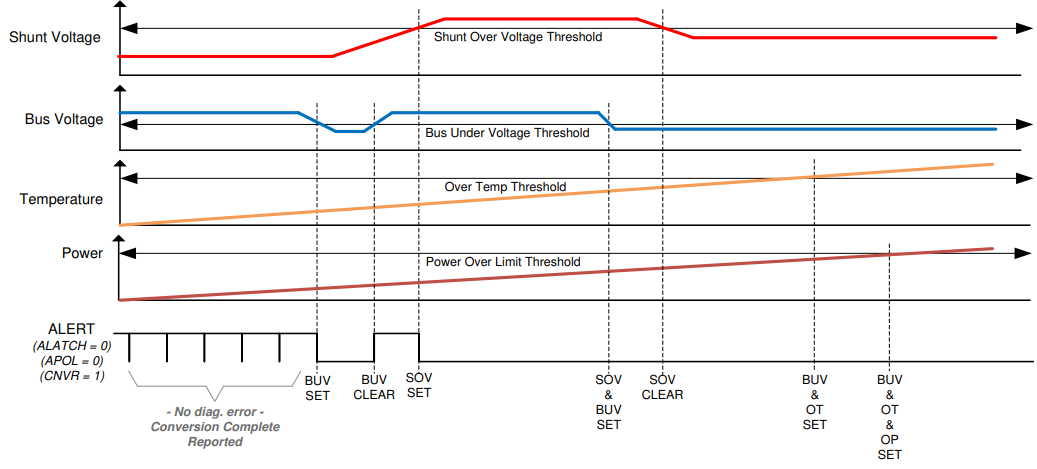
\includegraphics[width=0.8\textwidth]{Chap05/Figures/INA238_multi_alert.PNG}
	\caption{INA238 Multi-Alert Configuration}
	\label{fig:INA238_multi_alert}
\end{figure}
\section{Current Measurements Synchronization}
Section \ref{sec:INA238} described the very detailed view of INA238/INA2xx sensors, the essence of explaining INA is the most competitive solution for current measurements and it is the main pillar in this project to acquire current measurements and other several measurements(Shunt Voltage, Bus Voltage, ALERT). Among all measurements synchronizing the current measurements is the nail hitting. The following sections will brief different approaches to synchronize the current measurements.

\subsection{Simultaneous Write and Sequential Read :}
Thanks to the INA238/INA2xx multi-addressing functionality \cite[p.18]{INA238_User_Datasheet}, INA operates through I2C and the address of the INA can be configured by address lines A0 and A1 pulling to Vdd or GND. Figure \ref{fig:INA2xx_Simultaneous_Write_and_Sequential_Read}shows the Simultaneous Write and Sequential Read approach. Configure all the INAs (Write Control register) simultaneously by keeping all the INA addresses the same. Address configuration can be done, by the controller. As soon as write is done all the INAs start current acquisitions and report measurements at the same instant. For reading the current measurements, configure sensor address lines to different addresses(for instance 0x40,0x41,0x44,0x44, and so on) and read current measurements sequentially from each  INA.

\begin{figure}
    \centering
    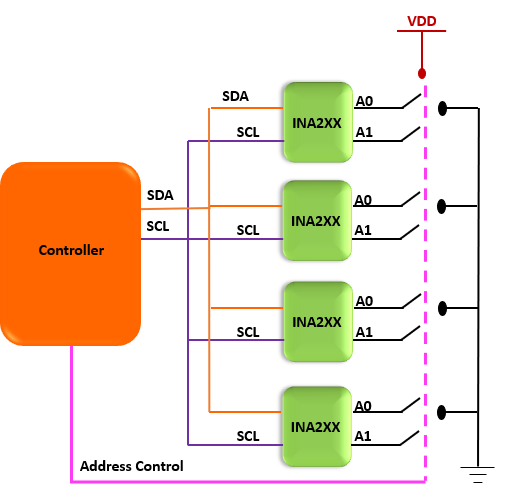
\includegraphics[width=0.4\textwidth]{Chap05/Figures/INA_MultiWrite.PNG}
    \caption{INA2xx Simultaneous Write and Sequential Read}
    \label{fig:INA2xx_Simultaneous_Write_and_Sequential_Read}
\end{figure}

"Simultaneous Write and Sequential Read" \ref{fig:INA2xx_Simultaneous_Write_and_Sequential_Read} approaches are reliable only for low precision and sequential data storage applications. SoC estimation is dealing with real-time current flowing in the battery, let's say a case where we write all sensors at the same time parallelly by considering the acknowledgment but this acknowledge could be sent by any one of the sensors if any one sensor dropped in between writing the data (configuring) controller can not differentiate. The controller only gets to know the sensor is not configured or dropped after it samples the first current data. Unfortunately, by that time the battery balancing might have already started if we do not receive current measurement data from anyone's sensor we might be in deep trouble. Simultaneous Write and Sequential Read are simple to implement but it is not robust and reliable for BMS applications.

\subsection{Synchronizing by Delayed Measurements  }
Depending on the MODE bits that have been specified and set in the ADC CONFIG register, the INA238 can measure the shunt voltage, bus voltage, die temperature, or any combination of these. This enables the user to further tune the monitoring function to meet the demands of the particular application by choosing modes to convert simply the shunt voltage or bus voltage.
\begin{figure}
    \centering
    \includegraphics[width=0.9\textwidth]{Chap05/Figures/INA_synchronization_alert.PNG}
    \caption{INA2xx Delayed Synchronization}
    \label{fig:INA_synchronization_alert}
\end{figure}

The INA238 conversion can be delayed to synchronize with other system components by setting the CONVDLY bits in the CONFIG register to a value between 0 (no delay) and 510 ms. The conversion delay resolution in programming is 2 ms. By default, the conversion delay is set to 0.As soon as the measurement conversion is complete the INA2xx ALERT pin asserts. Figure \ref{fig:INA_synchronization_alert} shows synchronizing the 3 sensors by writing the sequential delay for instance first sensor has a conversion delay of 2ms subsequently adding other sensors' conversion delay (INA1 delay = INA2 delay + INA3 delay + 2ms ). At the end of the 10ms all the sensors sample at the same time, finish the conversion and assert the alert pin.  As soon as the ALERT is asserted the controller interrupts will trigger and the controller will read the data from the sensors sequentially. The point here is not reading the data sequentially or parallel important is all the sensors must sample the current at the same instance time.

\paragraph{Implementation of Synchronizing by Delayed Measurements Algorithm:}\label{sec:INA2XX_synch_delayed_method}
\begin{itemize}
    \item Send to three INAs: the config alert command (bit 14, register Bh) and sets the CONVDLY (bits 13-6 register 0h), which is the delay for initial ADC conversion. ​
    \item When START ACQUISITION command is sent, the INA waits the time specified by CONVDLY ​before starting the conversion.​
    \item CONVDLY INA 1 = 10 ms, ​CONVDLY INA 2 = 6 ms, ​CONVDLY INA 3 = 2 ms​
    \item Two Timers are used to send the start acquisition command: Timer 1 = 4ms, Timer 2 = 4ms​
    \item As two timers finish writing controller wait for ALERT interrupt to read data from sensors
\end{itemize}

Figure \ref{fig:INA_synchronization_alert} shows the three INAs synchronize current measurement current, each INA triggered with a different delay to acquire data at the end of 10ms all the INAs are asserted alert signals. The sque of the ALERT of the INAs is quite impressive because they have responded with arround 10us of sque.

So on and so forth the above sections briefed about the current sensor, features, and synchronizing methods. This section will put a more detailed view of one of the current measurement applications from BMS architecture, Power analyzer emulation, and current measurement synchronization.

\section{Balancing Current Measurement}

As discussed in chapter \ref{ch:Architecture_Active_Balancing_BMS} active balancing architecture \ref{fig:BMS Architecture}the controller will operate the DC/DC converter either in buck or boost mode depending on the unbalanced node. The output current of the DC/DC converter is the total balancing current that needs to flow from the battery node to the pack or vice versa. DC/DC converter input and output both have the shunt resistor \ref{fig:BMS Architecture} where INAs are coupled with them to measure the current. 
All the currents in the architecture \ref{fig:BMS Architecture} are measured with the power analyzer setup as briefed in chapter \ref{fig:Battery_Pack_modeling_Architec},\ref{algo:PowerAnalyzer_Modeling}(Measurement view), and all the INAs synchronized with the "INAs delayed measurement algorithm" approach as mentioned in section \ref{sec:INA2XX_synch_delayed_method}. Though, we have several currents(Charging/Discharging TOP and bottom current, DC/DC converter low and high side currents) to talk about in the architecture \ref{fig:BMS Architecture} I would like to stress the DC/DC output current more! \ref{fig:Battery_Balancing_Current}. 
Because the output current of the DC/DC converter is the balancing current that can flow from the battery node to the battery pack or vice versa, which is one of the main currents that determine the battery SOC(charging and discharging excluded in this example). 
As the balancing current reaches the threshold current (shunt current threshold set by the user Figure \ref{fig:Battery_Balancing_Current}) ALERT will be asserted by the sensor (Section \ref{sec:INA238})  and the controller will monitor the DC/DC output shunt resistor current sensor and drop the balancing current below the threshold and maintains the same current until the balancing timer period ends. 

\begin{figure}
    \centering
    \includegraphics[width=0.6\textwidth]{Chap05/Figures/ShuntCurrent.png}
    \caption{Battery Balancing Current}
    \label{fig:Battery_Balancing_Current}
\end{figure}

\section{Summery of Chapter \ref{ch:Current_Measurement}}

Chapter \ref{ch:Current_Measurement} provided me an opportunity to explore different kinds of current measuring sensors for the BMS application and synchronize current measurements, after a deep analysis finally we landed with INA2xx series sensors. In section \ref{sec:INA238}, I took the advantage of explaining deeply about the current sensor, because most of the measurements and decisions are taken by the controller depend on the current sensor during the balancing for instance balancing current, balancing node voltage, balancing current thresholds, bus voltage threshold, and so on. INA current sensor ALERT signal configuration gave an extensive chance to explore the synchronization of the current measurement estimating the battery SoC. Battery balancing current results (Figure \ref{fig:Battery_Balancing_Current}) measured through the power analyzer model will interpolate the BMS architecture discussed in chapter \ref{ch:Architecture_Active_Balancing_BMS} to the Powel Analyzer architecture in chapter 4. This chapter can also become the fundamental pillar for chapter 5 to estimate the SOC with several algorithms (synchronization with Delayed Measurements and Parallel Wite; Sequential Read).
\thispagestyle{empty}
\cleardoublepage
% % % % % % % % % % % % % % % % % % % % % % % % % % %
% % % % % % % % % % % % % % % % % % % % % % % % % % %
\chapter{Battery Modeling and Emulation}\label{ch:Battery_Modeling_Emulation}
The \textit{Battery} is a complex composition of lethal chemicals that are very hard to handle in terms of safety and maintenance. So, is those petroleum vehicles safe? No, Not at all petroleum products and vehicles are much more dangerous not only in terms of environmental pollution it in terms of safety and measures. Then we should raise the question of what stopping modern engineers to transition from petroleum engines to Battery vehicles. And which wall stopping us from battery usage? Well, to answer all the above questions we need to look back at the evolution of vehicles, the petroleum vehicle fetus came to this world nearly a century ago. Engineers thoroughly studied and learned how to handle petroleum products and petroleum vehicles. Undoubtedly, EVs are the gift of modern technology, but it is essential to study institutionally the battery characteristics and the testing.

It is the prime responsibility of every Electrical engineer who works in EVs/Battery systems to ensure the safety of mankind. Considering all the facts, I have decided to make safety and sophisticated system for engineers to test the BMS and play with BMS without interacting with the physical batteries. The \textit{Part I} of Chapter \ref{ch:Battery_Modeling_Emulation} gives more elaboration about the battery modeling and battery constructional theory. \textit{Part II} facilitates understanding of Battery model implementation and BMS simulation through coding.

\section{Battery Modeling}\label{sec:Batt_Modeling}
This section explains the principles of a technique for calculating the state of charge (SOC) of lithium-ion batteries using two different equivalent circuit designs. It discusses how to use typical measurements to determine these circuits' parameters. The comparison of measurement and computation results reveals good agreement. The first step ignores the effects of temperature and battery age on these parameters \cite{UKEMPT_AHMAD2012}.
\\
The Ampere-counting (Columb counting) method can be used to identify the state of charge (SOC) of a battery if a defined full charge occurs regularly. This technique is based on the amount of charge that is put into or taken out of the battery. The error in the SOC estimation can grow too big and a better solution needs to be discovered in cases where a defined full charge of the battery cannot occur frequently.
A lithium-ion battery's open circuit voltage (OCV) determines the SOC; however, as shown in the figures, this method has an issue with the battery's dynamics.
The electrochemical reactions that occur in a cell prevent the OCV from being measured at the battery terminals. It is necessary to theoretically model the dynamics so that the OCV or SOC may be determined by measuring simply the battery voltage and current at the terminals of the battery. It is necessary to utilize an analogous circuit design for the battery cell for this purpose, and characteristic measurements must be employed to identify the parameters.
\\
This section presents three models: the internal resistance model (IR)\ref{fig:Battery_Equivalent_circuit}(a), the one-time constant model (OTC) \ref{fig:Battery_Equivalent_circuit}(b), and the two-time constants model (TTC) \ref{fig:Battery_Equivalent_circuit}(c). The presented models, which serve as the basis for the model-based SOC calculation, are also evaluated for validity by making comparisons between the model-based simulation data and the measured data\cite{UniPadua_Giacomo}.

\begin{figure}[h]
	\centering
	\includegraphics[width=0.5\textwidth]{Chap06/Figures/Batt_Ckt.PNG}
	\caption{Battery equivalent circuit diagrams. (a) internal resistance 
    model (IR), (b) one-time constant model (OTC), (c) two time 
    constants model (TTC) \cite{UKEMPT_AHMAD2012},\cite{UKEMPT_AHMAD2012} }
	\label{fig:Battery_Equivalent_circuit}
\end{figure}

\subsection{Nomenclature of Battery Model}
\begin{enumerate}
	\item \textbf{\textit{\underline{Open Circuit Voltage(OCV) }:}} OCV is measured at the battery's open circuit terminal voltage at various SOC points when the battery is in equilibrium. A polynomial equation is used to determine the nonlinear relationship between SOC and OCV. The figure \ref{fig:Battery_OCV_Vs_Soc} displays an OCV subsystem. Because SOC directly affects OCV's value, the OCV subsystem includes a SOC computation component. The value of OCV controls the regulated voltage source. The voltage curve of the pulse discharge test (PDT) during relaxation can be used to determine the OCV value\cite{Batt_Modeling_Kharisma}.
	\item \textbf{\textit{\underline{Internal Resistanse (R0) }:}} Internal resistance results in a voltage drop in the equivalent circuit. Fig. \ref{fig:Battery_Equivalent_circuit}(a), displays the value of the subsystem R0
	as a function of the input current and SOC. A switchable resistor
	utilized to transmit a resistor's internal value's physical signal.
	From this, one can calculate the amount of internal resistance.
	Instantaneous voltage following the release of the current pulse. 
	The optimal 2-D lookup table is selected using
	the interpolation-extrapolation lookup method for R0's value\cite{Batt_Modeling_Kharisma}.
	\item \textbf{\textit{\underline{Transient Response (R1,C1,R2,C2) }:}} Transient response in this model is represented by RC.
	The transient model is again classified based on the time constant for instance $R1\times C1 = \tau 1$ is a one-time constant model and $R2\times C2 = \tau 2$  is the two-time constant model; Figure \ref{fig:Battery_Equivalent_circuit}(b) and Figure \ref{fig:Battery_Equivalent_circuit}(c). Increasing the Time constant model will serve as a realistic model battery\cite{Batt_Modeling_Kharisma}.
\end{enumerate}

\begin{figure}[h]
	\centering
	\includegraphics[width=0.5\textwidth]{Chap06/Figures/Batt_OCV_SOC.PNG}
	\caption{Battery OCV Vs Soc for SLPB120216216 Cell \cite{UKEMPT_AHMAD2012}}
	\label{fig:Battery_OCV_Vs_Soc}
\end{figure}

\subsection{IR Model :}
the IR model as shown in Figure r\ref{fig:Battery_Equivalent_circuit} (a), and 
described by Equation \ref{eq:Batt_IR_equation} implements an ideal voltage 
source VOC that represents the open-circuit voltage (OCV) 
of the battery, and an ohmic resistance to describe 
the internal resistance \cite{UKEMPT_AHMAD2012}. Both resistance and open-circuit 
voltage VOC are functions of SOC, state of health (SOH) 
and temperature. $I_{Batt}$ is the battery output current with a 
positive value when discharging, and a negative value when 
charging, $V_{Batt}$ is the battery terminal voltage\cite{UKEMPT_AHMAD2012}.

\begin{equation}\label{eq:Batt_IR_equation}
    V_{Batt} = V{OC} - R_{0}\times I_{Batt}
\end{equation}
Given that the transient is not represented by the IR model
Lithium-ion cell behavior is not suited for the
precise SOC calculation for any dynamical operation
(variable load).

\subsection{One-Time Constant Model }
A parallel RC is added by the OTC model.
Network connected in series to the IR's internal resistance R0
model to approximate the lithium-ion battery's dynamic behavior.
As shown in Figure \ref{fig:Battery_Equivalent_circuit} (b), it mainly 
consists of three parts including the voltage source $V_{OC}$, the 
ohmic resistance R0, and $R_{OTC}$,$C_{OTC}$ to describe the battery 
transient response during charging or discharging. $\textit{V}_{OTC}$ is 
the voltage across $C_{OTC}$; $i_{OTC}$ is the current that flows in 
$C_{OTC}$ \cite{UKEMPT_AHMAD2012} $\dot{\textit{V}_{OTC}}$ is the iterative voltage of OTC model. The electric behavior of the OTC model can be 
expressed by Equations \ref{eq:OTC_Voltage } and \ref{eq:OTC_Batt_Voltage } \cite{UKEMPT_AHMAD2012} in continuous time \cite{UniPadua_Giacomo}: 

\begin{equation}\label{eq:OTC_Voltage }
    \dot{ V_{OTC}} = \frac{-1}{R_{OTC}\times C_{OTC}} V_{OTC} + \frac{1}{C_{OTC}} i_{Batt}
\end{equation}
\begin{equation}\label{eq:OTC_Batt_Voltage }
    V_{Batt} = V_{OC} -  \frac{1}{C_{OTC}} V_{OTC} - R_{0}\times i_{Batt}
\end{equation}
The equation\ref{eq:Discrete_OTC_Voltage } and \ref{eq:Discrete_OTC_Batt_Voltage } (where: $T_S$ sampling period, $T_s$ and $\tau_{OTC}$  time constant. ) represents the discrete time voltages of the one-time constant model, They are very much helpful for the advanced algorithms to calculate the SoC such as Kalman, Extended Kalman etc.
\begin{equation}\label{eq:Discrete_OTC_Voltage }
    V_{OTC,k+1} = e^{\frac{-T_{s}}{\tau_{otc}}} V_{OTC,k} + R_{OTC}\left(1- e^{\frac{-T_{s}}{\tau_{otc}}}\right) i_{Batt,k}
\end{equation}
\begin{equation}\label{eq:Discrete_eOTC_Batt_Voltage }
    V_{Batt,k} = V_{OC}(SOC_{k}) -  V_{OTC,k} - R_{0}\times i_{Batt}
\end{equation}

\subsection{Two-Time Constant Model }
Model TTC, It has been discovered that the battery exhibits a significant variation between the short- and long-term transient behavior based on observation of the battery output voltage when the battery output current is zero (no load). Therefore, the OTC model cannot adequately describe the dynamic properties.
\\
An additional RC network is connected in series with the OTC circuit to create the TTC circuit model, which increases the flexibility of the OTC model.
As shown in Figure \ref{fig:Battery_Equivalent_circuit} (c), the TTC circuit is 
composed of four parts: voltage source $V_{OC}$, ohmic 
resistance $R_{O}$, $T_{TTC1}$ and $C_{TTC1}$ to describe the short term 
characteristics, $R_{TTC2}$ and $C_{TTC2}$ to describe the long term 
characteristics. $v_{TTC1}$ and $v_{TTC2}$ are the voltages across $C_{TTC1}$
and $C_{TTC2}$ respectively\cite{UKEMPT_AHMAD2012}. $i_{TTC1}$ and $i_{TTC2}$ are the outflows 
currents of $C_{TTC1}$ and $C_{TTC2}$ respectively \cite{UniPadua_Giacomo}. 

Equations \ref{eq:TTC_Voltage1 }, \ref{eq:TTC_Voltage2 }, and \ref{eq:TTC_Batt_Voltage } can be used to represent the electrical behavior of the TTC circuit in continuous time.
\begin{equation}\label{eq:TTC_Voltage1 }
    V_{TTC1} = \frac{-1}{R_{TTC1}\times C_{TTC1}} V_{TTC1} + \frac{1}{C_{TTC1}} i_{Batt}
\end{equation}
\begin{equation}\label{eq:TTC_Voltage2 }
    V_{TTC2} = \frac{-1}{R_{TTC2}\times C_{TTC2}} V_{TTC2} + \frac{1}{C_{TTC2}} i_{Batt}
\end{equation}
\begin{equation}\label{eq:TTC_Batt_Voltage }
    V_{Batt} = V_{OC} -  V_{TTC1} - V_{TTC2} - R_{0}\times i_{Batt}
\end{equation}

The TTC model equations' description in discrete time is given by Equations \ref{eq:Discrete_TTC_Voltage1 }, \ref{eq:Discrete_TTC_Voltage2 } and \ref{eq:Discrete_TTC_Batt_Voltage }:
\begin{equation}\label{eq:Discrete_TTC_Voltage1 }
    V_{TTC1,k+1} = e^{\frac{-T_{s}}{\tau_{TTC1}}} V_{TTC1,k} + R_{TTC1}\left(1- e^{\frac{-T_{s}}{\tau_{TTC1}}}\right) i_{Batt,k}
\end{equation}
\begin{equation}\label{eq:Discrete_TTC_Voltage2 }
    V_{TTC2,k+1} = e^{\frac{-T_{s}}{\tau_{TTC2}}} V_{TTC2,k} + R_{TTC2}\left(1- e^{\frac{-T_{s}}{\tau_{TTC2}}}\right) i_{Batt,k}
\end{equation}
\begin{equation}\label{eq:Discrete_TTC_Batt_Voltage }
    V_{Batt,k} = V_{OC}(SOC_{k}) -  V_{TTC1,k}-  V_{TTC2,k} - R_{0}\times i_{Batt}
\end{equation}


\subsection{Estimation of the Model Parameters}\label{sec:Batt_model_parameters_estimation}
This section demonstrates the process for estimating model parameters based on battery readings. First, the effects of temperature and aging are disregarded. At a constant temperature of 25°C, the experimental parameter identification of the battery was carried out using recently manufactured, unused cells. Figure \ref{fig:Battery_Current_Pulse} shows the typical Battery Charging and discharging behavior for the large current pulse. A continuation of this work will take into account the effects of temperature and aging.
\subsubsection{Charging and Discharging :}
Figure \ref{fig:Battery_Current_Pulse} displays the voltage and current output characteristic curves of a battery during charging and discharging. 
Following is a description of the various curve subintervals:

\begin{itemize}
	\item \textbf{Subinterval $S_0 (t < t_0 )$ :} In this subinterval the battery 
	the output current can be assumed to zero over a sufficient 
	time, though the output voltage can reach the open circuit 
	voltage value $V_{OC}(SOC_0)$, and while the output current is 
	zero the SOC value is constant \cite{UKEMPT_AHMAD2012},\cite{UniPadua_Giacomo}.
	\item \textbf{Subinterval $S_1 (t_0 \leq t \leq  t_1 )$ :}  In this subinterval the battery 
	is discharged with a constant current $I_{discharge} > 0$, first  
	a steep decrease in the battery output voltage can be seen 
	due to the internal resistance R0, and then it continues to 
	decrease exponentially controlled by the OCV (as the SOC 
	is decreasing)\cite{UKEMPT_AHMAD2012}. 
	\item \textbf{Subinterval $S_2 (t_1 \leq t \leq  t_2 )$ :} In this subinterval the battery 
	output current $i_{Batt} = 0$, so the battery output voltage at first 
	will have a steep increase due to $R_0$, and then it shows an 
	exponential increase until it reaches $V_{OC}(SOC_1)$. 
	\item \textbf{Subinterval $S_3 (t_2 \leq t \leq  t_3 )$ :} In this subinterval the battery 
	is charged with a constant current $I_{charge} < 0$; at first a steep 
	increase in the battery output voltage can be seen due to 
	internal resistance $R_0$, and then it continues to increase 
	exponentially controlled by the OCV (as the SOC is 
	increasing)\cite{UKEMPT_AHMAD2012}.
	\item \textbf{Subinterval $S_4 (t_3 \leq t \leq  t_4 )$ :} In this time subinterval the battery 
	output current $i_{Batt} = 0$, so the battery output voltage at first 
	will have a steep decrease due to $R_0$, and then it has an 
	exponential decrease until it reaches $V_{OC}(SOC_2)$ \cite{UKEMPT_AHMAD2012}. 
\end{itemize}

\begin{figure}[h]
	\centering
	\includegraphics[width=0.5\textwidth]{Chap06/Figures/Batt_Pulsed_current_char.PNG}
	\caption{Characteristic waveforms for battery output voltage and current during charging and discharging of lithium-ion cells.}
	\label{fig:Battery_Current_Pulse}
\end{figure}

\paragraph{Ohmic Resistance :} 
The voltage drop across R0 at the 
first time instant when charging ($V_2$) respectively 
discharging ($V_0$) can be taken to calculate $R_0$ \cite{Internal_Resistance_LIPO_Batt_Gogoana}, according 
to Equation \ref{eq:Batt_Ohmic_Resistance}: 

\begin{equation}\label{eq:Batt_Ohmic_Resistance}
	R_0 =\begin{cases}
	  \frac{V_0}{I_{discharge}}, & \text{: for discharge}.\\
	  \frac{- V_2}{I_{discharge}}, & \text{: for charge}.\\
	\end{cases}
\end{equation}

\paragraph{Estimation of the OTC Model Parameters :} 
in this step 
battery output voltage measurements during the 
subintervals S2 and S4 are used, as in these subintervals 
OCV is constant\cite{Internal_Resistance_LIPO_Batt_Gogoana}, and the battery output voltage is just 
driven by the dynamic characteristics of the battery. The 
output voltage $v_{Batt}$ during S2 and S4 can be calculated 
according to the OTC model by setting $i_{Batt}$ to zero in 
Equations \ref{eq:OTC_Voltage } and \ref{eq:OTC_Batt_Voltage }, then solving the differential equation as 
shown in Equation \ref{eq:Batt_OTC_Diff_Eq_Sol} \cite {UKEMPT_AHMAD2012}:

\begin{equation}\label{eq:Batt_OTC_Diff_Eq_Sol}
	\begin{cases}
	  S_2 : V_{Batt}(t) = V_{OC}(SOC_1) - v_{OTC}(t1) e^{\frac{-t}{\tau_{OTC}}} , & \text{:where,} \tau_{OTC} = R_{OTC}\times C_{OTC}.\\
	  S_4 : V_{Batt}(t) = V_{OC}(SOC_2) - v_{OTC}(t3) e^{\frac{-t}{\tau_{OTC}}}\\
	\end{cases}
\end{equation}

Estimating the values is necessary for the identification of OTC model parameters $V_{OC}(SOC_1),V_{OC}(SOC_2),v_{OTC}(t1),v_{OTC}(t3), \tau_{OTC}$  
in Equations \ref{eq:Batt_OTC_Diff_Eq_Sol}. A nonlinear least squares approach is used (also known as nonlinear data fitting) to find the values that best suit the relationship between the measurements and the nonlinear function, in this case, an exponential function, to estimate these parameters
$f(t) = A + Be^{-\alpha t}$ . \\

The vector of coefficients A, B, and $\alpha$ is the result of the nonlinear least squares algorithm. Through Equations \ref{eq:Batt_OTC_Least_Square_solution} to \ref{eq:Batt_OTC_C_OTC}, these coefficients will be used to calculate the OTC model parameters:

\begin{equation}\label{eq:Batt_OTC_Least_Square_solution}
	\begin{cases}
	  S_2 : V_{OC}(SOC_1) = A, v_{OTC}(t1) = B, & \text{:where,} \tau_{OTC} = \frac{1}{\alpha}.\\
	  S_4 : V_{OC}(SOC_2) = A, v_{OTC}(t2) = B,\\
	\end{cases}
\end{equation}

\begin{equation}\label{eq:Batt_OTC_T_charge_discharge}
	\begin{cases}
		T_{Charge} = t1 - t0\\
		T_{Discharge} = t3 - t2 \\
	\end{cases}
\end{equation}

\begin{equation}\label{eq:Batt_OTC_R_OTC}
	\begin{cases}
	  S_2 : R_{OTC} = \frac{v_{OTC}(t1)}{ \left( 1 - e^{\frac{- T_{Discharge} }{\tau_{OTC} }}\right) I_{Discharge}} \\
	  S_4 : R_{OTC} = \frac{v_{OTC}(t3)}{ \left( 1 - e^{\frac{- T_{Charge} }{\tau_{OTC} }}\right) I_{Charge}} \\
	\end{cases}
\end{equation}

\begin{equation}\label{eq:Batt_OTC_C_OTC}
	C_{OTC} = \frac{\tau_{OTC}}{R_{OTC}}
\end{equation}

\paragraph{Estimation of the TTC Model Parameters :} 

By considering the two RC networks in place of the OTC model's single RC network, the TTC model parameters can be calculated in the same manner as for the OTC model. Equations \ref{eq:Batt_TTC_Diff_Eq_Sol} can be used to define the output voltage of the TTC model for the subintervals S2 and S4. The experiments carried out on the LIPO Battery and the typical parameters of the Battery are shown in table 4.1.

\begin{equation}\label{eq:Batt_TTC_Diff_Eq_Sol}
	\begin{cases}
	  S_2 : V_{Batt}(t) = V_{OC}(SOC_1) - v_{TTC1}(t1) e^{\frac{-t}{\tau_{TTC1}}} - v_{TTC2}(t1) e^{\frac{-t}{\tau_{TTC2}}},&\tau_{TTC1} = R_{TTC1}\times C_{TTC1}.\\
	  S_4 : V_{Batt}(t) = V_{OC}(SOC_2) - v_{TTC1}(t3) e^{\frac{-t}{\tau_{TTC1}}} - v_{TTC2}(t3) e^{\frac{-t}{\tau_{TTC2}}},&\tau_{TTC2} = R_{TTC2}\times C_{TTC2}. \\
	\end{cases}
\end{equation}


\begin{table}[ht]\label{tb:SLPB120216216_Cell_Data }
	\begin{center}
		\begin{tabular}{|c|c|c|}
			\hline
			\multicolumn{2}{|c|}{{Typical Capacity }} & 53 Ah\\
			\hline
			\multicolumn{2}{|c|}{{Nominal Voltage}} & 3.7\\
			\hline
			\multicolumn{1}{|c|}{\multirow{2}{*}{Charge Condition}}& Max. Current & 53A\\ 
			\multicolumn{1}{|c|}{}& Voltage & 4.2V $\frac{+}{-}$ 0.03V\\
			\hline
			\multicolumn{1}{|c|}{\multirow{2}{*}{Discharge Condition}}& Max. Current & 159A\\
			\multicolumn{1}{|c|}{}& Peak Current & 290A\\
			\multicolumn{1}{|c|}{}& Cut-off Voltage & 3.0V\\
			\hline
		\end{tabular}
		\caption{SLPB120216216 Cell Data }
	\end{center}
	\label{tab:multicol}
\end{table}

Estimating the values is required for the TTC model's identification, $V_{OC}(SOC_1), V_{OC}(SOC_2), v_{TTC_1}(t1), v_{TTC_1}(t3), v_{TTC_2}(t1), 
v_{TTC_2}(t3), \tau_{TTC_1}  and  \tau_{TTC_2}$ in Equations \ref{eq:Batt_TTC_Diff_Eq_Sol}. In this 
case an exponential function with two-time constants $f(t)=A+Be^{-\alpha t}+Ce^{- \beta t}$ is used.
\\
The vector of coefficients A, B, C,$\alpha, and \beta$ is the result of the nonlinear least squares algorithm. Through Equations \ref{eq:Batt_OTC_Least_Square_solution} to \ref{eq:Batt_TTC_C_TTC}, these coefficients will be utilized to calculate all the TTC model's parameters. 

\begin{equation}
	\begin{cases}
	  S_2 : V_{OC}(SOC_1) = A 
	  S_4 : V_{OC}(SOC_2) = A
	\end{cases}
\end{equation}

\begin{equation}\label{eq:Batt_OTC_Least_Square_solution}
	\begin{cases}
	  S_2 :  v_{TTC1}(t1) = B, v_{TTC2}(t1) = C ,& \text{:} \tau_{TTC1} = \frac{1}{\alpha}.\\
	  S_4 :  v_{TTC1}(t3) = B, v_{TTC2}(t3) = C ,& \text{:} \tau_{TTC2} = \frac{1}{\beta}.\\
	\end{cases}
\end{equation}

\begin{equation}\label{eq:Batt_TTC_R_TTC1}
	\begin{cases}
	  S_2 : R_{TTC1} = \frac{v_{TTC1}(t1)}{ \left( 1 - e^{\frac{- T_{Discharge} }{\tau_{TTC1} }}\right) I_{Discharge}} \\
	  S_4 : R_{TTC1} = \frac{v_{TTC1}(t3)}{ \left( 1 - e^{\frac{- T_{Charge} }{\tau_{TTC1} }}\right) I_{Charge}} \\
	\end{cases}
\end{equation}

\begin{equation}\label{eq:Batt_TTC_R_TTC2}
	\begin{cases}
	  S_2 : R_{TTC2} = \frac{v_{TTC2}(t1)}{ \left( 1 - e^{\frac{- T_{Discharge} }{\tau_{TTC2} }}\right) I_{Discharge}} \\
	  S_4 : R_{TTC2} = \frac{v_{TTC2}(t3)}{ \left( 1 - e^{\frac{- T_{Charge} }{\tau_{TTC2} }}\right) I_{Charge}} \\
	\end{cases}
\end{equation}

\begin{equation}\label{eq:Batt_TTC_C_TTC}
	\begin{cases}
		C_{TTC1} = \frac{\tau_{TTC1}}{R_{TTC1}} \\
		C_{TTC2} = \frac{\tau_{TTC2}}{R_{TTC2}} \\
	\end{cases}
\end{equation}

\subsection{Experimental and Computational Results of SLPB120216216}
Cells made of lithium polymer by the producer Kokam were employed for the modeling and experimental experiments.
Table 4.1 shows several significant cell data. A battery test bench was established to determine the model parameters. Using short and long interruptions, a rectangular-shaped current signal must be applied to the battery on this test bench. It is also necessary to measure the voltage of the battery output. While the OTC and TTC model parameters must be determined during extended pauses, the battery's ohmic resistance R0 can be measured during small interruptions of the current signal.

\begin{figure}[h]
	\centering
	\subfigure[Ohmic Resistance $R_0 = f(SOC) @ Discharging $]{\includegraphics[scale=.8]{Chap06/Figures/Batt_DisCh_Ohmic_Resistance.PNG}}
	\qquad
	\subfigure[Ohmic Resistance $R_0 = f(SOC) @ Chareging $]{\includegraphics[scale=.8]{Chap06/Figures/Batt_Ch_Ohmic_Resistance.PNG}}
	\qquad
	\subfigure[Output Voltage of the Battery $@ Discharing$]{\includegraphics[scale=.8]{Chap06/Figures/Batt_DisCh_OutPut_Voltage.PNG}}
	\qquad
	\subfigure[Output Voltage of the Battery $@ Charging $]{\includegraphics[scale=.8]{Chap06/Figures/Batt_Ch_OutPut_Voltage.PNG}}
	\qquad
	\subfigure[Dynamic Resistance of the Battery  $R_{OTC}/R_{TTC1}/R_{TTC_2} = f(SOC) @ Discharging $]{\includegraphics[scale=.8]{Chap06/Figures/Batt_DisCh_Resistance.PNG}}
	\qquad
	\subfigure[Dynamic Resistance of the Battery $R_{OTC}/R_{TTC1}/R_{TTC_2} = f(SOC) @ Charging $]{\includegraphics[scale=.8]{Chap06/Figures/Batt_Ch_Resistance.PNG}}
	\qquad
	\subfigure[Dynamic Capacitance of the Battery  $C_{OTC}/C_{TTC1}/C_{TTC_2} = f(SOC) @ Discharging $]{\includegraphics[scale=.8]{Chap06/Figures/Batt_DisCh_Capacitance.PNG}}
	\qquad
	\subfigure[Dynamic Capacitance of the Battery $ C_{OTC}/C_{TTC1}/C_{TTC_2} = f(SOC)  @ Charging $]{\includegraphics[scale=.8]{Chap06/Figures/Batt_Ch_Capacitance.PNG}}
	\caption{LIPo Battery SLPB120216216 Simulated Results \cite{UKEMPT_AHMAD2012} }
	\label{fig:LIPO_Batt_SLPB120216216_Results}
\end{figure}
  
\section{Battery Emulation}

\textit{Part I} of the chapter \ref{ch:Battery_Modeling_Emulation} described extensively the LIPO Battery Modeling and equivalent circuit analysis. The \textit{Part II} of the chapter gives more extravagance to the Battery model implemented in real-time. \textit{Part II} will also talk about different instrumentation and configurations. I have used and python environment to implement the system, the reason behind choosing python as a coding environment is, python is a high-level used and most compatible with different instruments. The basis for implementing the battery model is the data that is collected for the SLPB120216216 by Ahmad RAHMOUN, Helmuth BIECHL. Gratitude to \textit{Ahmad RAHMOUN and Helmuth BIECHL} for their paper\cite{UKEMPT_AHMAD2012} \textit{"Modelling of Li-ion batteries using equivalent circuit diagrams"} this paper became the bedrock for this module implementation. Following the upcoming sections is the continuation of the \textit{Part I} battery modeling with the coding environment.

\begin{figure}[h]
	\centering
	\includegraphics[width=0.9\textwidth]{Chap06/Figures/Battery_Pack_modeling_Architec.PNG}
	\caption{Architecture of the Battery Pack Modeling/Emulation For BMS}
	\label{fig:Battery_Pack_modeling_Architec}
\end{figure}

\subsection{Fundamental Instruments For Battery Emulation }

Figure \ref{fig:Battery_Pack_modeling_Architec} shows the architecture of the Battery modeling and the emulation, for the external view the architecture looks very clumsy and dusky, but I have followed the modular approach in this architecture to extend the model to a one-time constant or two-time constant even three. The proposed architecture can handle multiple current sourcing, sinking, and measuring instruments without disturbing the overall system. Before diving into the architecture and modular approach, it is good to understand what kind of instruments can be used. And their specifications for the BMS applications. The following section can give brief information on the instruments and their configurations.

\subsubsection{Chroma :}
% \begin{figure}[h]
% 	\centering
% 	\subfigure[16CH Battery Cell Simulator 87001]{\includegraphics[width=0.4\textwidth]{Chap06/Figures/Chroma.PNG}}
%     \qquad
% 	\subfigure[Chroma Output Wiring to the BMS]{\includegraphics[width=0.4\textwidth]{Chap06/Figures/Chroma_Output_wiring.PNG}}
% 	\caption{16CH Battery Cell Simulator 87001}
% 	\label{fig:Chroma}
% \end{figure}
The 87001 16CH Battery Cell Simulator can simulate the cell to perform charge and discharge behavior for BMS testing. It can simulate up to 480 battery cells in series with voltage and current measurement functions. It can receive IPC's commands in real-time, store the measured values temporarily and return them to the IPC \cite{Chroma_UserManual}.Chroma has two communication one through the ethernet and CAN bus, for facilitating the modular and easy communication I preferred ethernet for this particular project, we can also use the can bus when we test the emulator with the real-time vehicle setup. Figure \ref{fig:Chroma}(a) shows the 16CH chroma which I have used in the lab.

\paragraph{Sepcifications of the Chroma :}

\begin{itemize}
    \item This simulator has built a DC Power Supply with 1Φ110~220V±10$\%$VLN input power.
    \item Each unit has 16 channels output that can set parameters, start and end time respectively.
    \item The channel can be a constant voltage source with a constant current function.
    \item Maximum 30 sets of 87001 simulators can be connected in series for use and can simulate the battery cell voltage of a 480-cell battery pack (2000V/4.2V) in series.
    \item High-precision output and measurement that are used in laboratories for testing product specifications and characteristics.
    \item No display panel and operation buttons but using LED lights to indicate the standalone unit status.
    \item Each channel has 2 current ranges (2 Current: (-5A~+5A, -0.5A~+0.5A) ).
    \item The operating interface uses the internet to give commands, control output measurement and read data via an external PC. The communication interface is Ethernet with SCPI protocol specification.
    \item Channels can be connected in series/parallel across a standalone unit with up to two batteries connected in parallel.
    \item Noise < 60db (output terminal 5V/5A/16CH)
    \item \textbf{Auto Range Select }
            \begin{itemize}
                \item The CC automatically switches to the proper range according to the set current.
                \item The CV automatically switches to the mapping range according to the upper limit current.
            \end{itemize} \ref{fig:Chroma}(a)
    \item \textbf{Current Range Select }
            \begin{itemize}
                \item When 5A is in use, performing CC(Constant Current) charge for 500uA may have a bigger error.
                \item When 500mA is in use, performing CC charge for 5A will prompt a warning and stop execution.
            \end{itemize}

    \item \textbf{Data Transmission :} The data transmission interval is 10ms * paralleled unit no. The minimum data transmission interval is Δ10ms for one unit and Δ20ms for two units, and so forth.
    
\end{itemize}

\paragraph{Output Wiring of the Chroma :}
% \begin{figure}[h]
% 	\centering
% 	\includegraphics[width=0.4\textwidth]{Chap06/Figures/Chroma_Output_wiring.PNG}
% 	\caption{Chroma Output Wiring to the BMS} 
% 	\label{fig:Chroma_Output_wiring}
% \end{figure}

\begin{itemize}
    \item The figure \ref{fig:Chroma}(b) is the parallel connection diagram of two simulators \cite{Chroma_UserManual}. (Same for serial connection.)
    \item The 87001 is a 4-wire measurement. The SENSE wire and BMS connection point should be as close as possible to the BMS input terminal to avoid voltage differences due to line losses.
\end{itemize}

\paragraph{Configuring the Chroma:}

For Programing the Chroma I took the help of the pyvisa library, which can use to interface with instruments using different protocols. The first setup is the NI (National Instrument) driver in PC to identify the instrument (install NI Max application in PC), through the NI driver, pyvisa can communicate through the VISA virtual port. The piece of code shows how to configure the visa port for the chroma(or any battery emulator commands that are more generalized) \cite{Chroma_UserManual}.

% \lstinputlisting[language=python]{Chap06/Code/Chroma.py}
\begin{lstlisting}[language=Python, caption=VISA parameters set for Chroma]
    #VISA commands for the Chroma
    set_visa_attribute(pyvisa.constants.VI_ATTR_MAX_QUEUE_LENGTH, 50)
    #Time Out Value 
    set_visa_attribute(pyvisa.constants.VI_ATTR_TMO_VALUE, 2000) 
    set_visa_attribute(pyvisa.constants.VI_ATTR_TERMCHAR_EN, 
                        pyvisa.constants.VI_TRUE)
    set_visa_attribute(pyvisa.constants.VI_ATTR_TERMCHAR, 0xA) 
    set_visa_attribute(pyvisa.constants.VI_ATTR_SEND_END_EN, 
                       pyvisa.constants.VI_TRUE) 
    
    set_visa_attribute(pyvisa.constants.VI_ATTR_SUPPRESS_END_EN, 
                       pyvisa.constants.VI_TRUE)
    set_visa_attribute(pyvisa.constants.VI_ATTR_FILE_APPEND_EN, 
                       pyvisa.constants.VI_FALSE) 
    set_visa_attribute(pyvisa.constants.VI_ATTR_IO_PROT, 1) 
    set_visa_attribute(pyvisa.constants.VI_ATTR_TCPIP_NODELAY, 
                       pyvisa.constants.VI_TRUE) 
    set_visa_attribute(pyvisa.constants.VI_ATTR_TCPIP_KEEPALIVE, 
                       pyvisa.constants.VI_TRUE)
\end{lstlisting}

The following code explores the basic programming of the chroma for BMS application:

\begin{lstlisting}[language=Python, caption=Basic BMS Program for Chroma]
    #Basic Program for Chroma to configure the cells
    chroma.query('*IDN?\n') # identify the instrument
    #Query the output sampling time
    chroma.query('SIM:CONF:SAMP:TIME?\n') 

    #number of BMS(each Chroma is One BMS) are parallel
    chroma.write(f'SYST:SLAVE:PARA {self.noOfBMS}\n')
    chroma.write(f'SYST:SLAVE:SCAN {self.noOfBMS}\n')

    #Chroma Status commands
    chroma.query('SYSTem:FRAME:STATe? 0\n')
    chroma.query('SYST:FRAME:CHAN:STATe? 1\n')
    chroma.query('SYST:FRAME:CHAN:NUMB? 0\n')
    chroma.write('SIM:CONF:CHAN:ACT 65535\n')
    chroma.write('SIM:CONF:CLE\n'

    ''' BMS configurations '''
    #Number of the BMS 1
    chroma.write(f'SIM:CONF:BMS:NUMB {noOfBMS}\n')
    #No cells use in the BMS testing #1 BMS , #2 Cells 
    chroma.write(f'SIM:CONF:CELL:NUMB {noOfBMS},{noOfBMSCells}\n')
    #BMS 1, CellStart 1, Cellend 2, 
    # Cell parallel to the channel1 , # Current Range 2  - 5.0 A
    chroma.write(f'SIM:CONF:CELL:PARA {noOfBMS},{noOfBMS},
    {noOfBMStestingCells},{paralleBMSchannel},{cellCurrent_5A}\n') 

    ''' Output Parameters Set '''

    ''' # BMS start  1 ,# BMS end 1 ,#set the start cell 1, 
    # set the end cell 1, # set the cell voltage 4.0 ,
     # set the Current of the cell 0.5A '''

    chroma.write(f'SIM:PROG:CELL {noOfBMS},{noOfBMS},{cellNo},
    {cellNo},{cellVoltage},{cellCurrent5A}\n') 

    # Switch on all the cells immediately
    chroma.write('SIM:OUTP:IMM\n') 

    '''### check if there is any error 
    in the Chroma while setting the voltages 
    ### if there is no error enable
     all the cells outputs''' 

    time.sleep(10)
    # Check the configuration Error 
    self.chroma.query('SYST:ERR?\n')

    # Switch on all the cells
    self.chroma.write('SIM:OUTP ON \n')  
    time.sleep(1) # give some time to switch on the emulator 

\end{lstlisting}

The above-attached code is just a basic code for the BMS application which can give a better idea about the basic chroma(Battery emulator) for more SCPI commands of the chroma follow the user manual\cite{Chroma_UserManual} and for the detailed class-based skeleton follow \textcolor{blue}{here}. %\href{}{here}.

\paragraph{Response Time of the Chroma :}
During battery, balancing it is essential to capture the battery voltage, in reality, this is not the problem because we might be dealing with the actual batteries which do not need voltage updates to the batteries. When we deal with any instruments (battery emulators) it is essential to update the battery (Cell) voltages and battery currents. In this particular project, chroma is used as the battery emulator. Chroma is being communicated through a python script to update its parameters via ethernet. The fundamental response time of the chroma for every request is 10ms, that being said for our application few 100ms time duration is good enough for calculating the batteries SoC. Perhaps I made some demonstration of the chroma response time and the number of packets, figure \ref{fig:Chroma_Packet_delay} shows the round robbin delay of 8 cells current and voltage fetch from chroma.
The results are quite adequate, over 10k packet request chroma has missed one or two chances of delaying 500ms, which still satisfies a few million packets.

\begin{figure}[h]
	\centering
	\includegraphics[width=0.5\textwidth]{Chap06/Figures/Chroma_Packet_delay.png}
	\caption{Chroma Response Time for Voltage and Current Request }
	\label{fig:Chroma_Packet_delay}
\end{figure}

\subsubsection{Load/Charger :}

In the setup\ref{fig:Battery_Pack_modeling_Architec} load or charger is used across the series cells (battery pack) which can only supply current or sink current from the pack. For this particular architecture, I have preferred e Keysight N6705 DC Power Analyze as a load or charger. All the controls have been passed through the power analyzer module through the script.

\paragraph{ Keysight N6705 DC Power Analyzer :}

The Keysight N6705 Figure \ref{fig:keysight_n6705_DMM_34460A}(a) DC Power Analyzer is a multipurpose power system that combines the capabilities of an oscilloscope, a data logger, and a DC voltage source with numerous outputs \cite{Keysight_N6705_DC_Power_Analyzer}.

The Keysight N6705 has up to four programmable outputs as a multiple-output DC source. The power levels of the available power modules range from 20 W to 500 W, with different voltage and current combinations, and they offer a wide range of performance capabilities. Additionally, each output can generate arbitrary (Arb) waveforms, allowing you to program. Standardized voltage and current waveforms, or create your own. With Keysight N678xA SMUs (Source/Measure Units) have a multi-quadrant power mesh with distinct voltage and sources of current priority \cite{Keysight_N6705_DC_Power_Analyzer}.

% \begin{figure}[h]
% 	\centering
% 	\subfigure[4 Channel keysight N6705 Power Supply]{\includegraphics[width=0.4\textwidth]{Chap06/Figures/keysight_n6705.PNG}}
%     \qquad
% 	\subfigure[Chroma Output Wiring to the BMS]{\includegraphics[width=0.4\textwidth]{Chap06/Figures/DMM_34460A.PNG}}
% 	\caption{ keysight N6705 Power Supply and DMM 34460A }
% 	\label{fig:keysight_n6705_DMM_34460A}
% \end{figure}

The Keysight N6705's Meter View shows the average output voltage and current as a measurement system. Scope View, which you can modify using the vertical and horizontal sliders, displays waveforms. The Data Logger View records average and peak voltage and current measurements over a long period and plots the data \cite{Keysight_N6705_DC_Power_Analyzer}.

The setup allows configuring the DC power supply as a charger or load, by setting the current direction.  The following program shows the typical program for load/chargers:

\begin{lstlisting}[language=Python, caption=Load/Charger Configuration for Keysight N6705's]

    #find the resource
    rm = pyvisa.ResourceManager()
    #open the instrument by the id 
    loadCh = rm.open_resource('USB0::0x0957::0x0F07:
                    :MY50000622::INSTR')
    #Identify Keysight N6705's
    loadCh.query('*IDN?\n')
    
    '''Configure Power analyzer channels 1 and 3 in 
    2 quadrants to sink or source current; that presumes 
    Load or Charger'''
    loadCh.write('EMUL PS2Q,(@1,3)')

    # Eneable current priority for channels 1 and 3
    loadCh.write('FUNC CURR,(@1,3)')
    
    # Set currnet range for 1 and 3 channel  1Amp
    loadCh.write('SOUR:CURR:RANG 1.02,(@1,3)')
    loadCh.write('CURR 1,(@1,3)')
    
    #Set Voltage limt for 28V
    loadCh.write('VOLT:LIM 28,(@1,3)')

    # Switch on Channel 1 and channel 3
    loadCh.write('OUTP ON,(@1,3)')
    
\end{lstlisting}

The above program is just an example of programming channel 1 and channel 3, we can couple the power supply channels for programming and trigger at the same time ($OUTP:COUP:CHAN$ \textit{1,2 ; Couple channel 1 and 2}). For more details and programming examples, refer to the keysight N6705B datasheet \cite{Keysight_N6705_DC_Power_Analyzer}.

\subsubsection{Meter View :}
The proposed architecture \ref{fig:Battery_Pack_modeling_Architec} encounters a meter view, which meter view allows the collaboration of various measuring instruments which can be directly controlled. A meter view in the architecture is directly controlled by the power analyzer module. Measurements include DC/DC converter input/output current measurements, and battery pack current measurements. The current measurement setup in the system is very much critical, hence we can measure the shunt voltage, and we can calculate the current flow (if shunt resistance is known). Measurement view is so much modular that we can have as many measuring instruments in the setup, and we log the data without disturbing the setup.
In the architecture, keysight 34470A DMM  \ref{fig:keysight_n6705_DMM_34460A}(b) has been employed for shunt voltage measurements (Battery Pack Current, DC/DC input/output current; Fig \ref{fig:BMS Architecture}). The following sections will give more detailed information about the multimeter and configuration.

\paragraph{Digital Multimeters 34460A :}

% \begin{figure}[h]
% 	\centering
% 	\includegraphics[width=0.4\textwidth]{Chap06/Figures/DMM_34460A.PNG}
% 	\caption{Keysight Technologies Digital Multimeters 34460A}
% 	\label{fig:keysight_DMM_34460A}
% \end{figure}

The only completely drop-in, SCPI-compatible alternative to the 34401A DMM in the market is the Digital Multimeters 34461A \cite{Keysight_34460A_DMM}. Although some other DMMs claim to be 34401A SCPI compatible, they only support a limited number of SCPI commands. The same design team that produced the 34401A also produced the Truevolt DMMs. When developing the Truevolt family of DMMs, the team kept 34401A measures, dependability, and familiarity in mind. Consequently, people may use it without having to spend hours learning how.
The following basic programming for DMM gives more insights into communication and configuration for measurement setup :

\begin{lstlisting}[language=Python, caption=DMM Keysight 34401A's Meauring/Configuration ]
    rm = visa.ResourceManager()
    ''' usb_id='USB0::0x2A8D::0x1301::MY57216238::INSTR' VISA id of DMM 
    Open VISA port
    '''
    mul_34461A = rm.open_resource(usb_id)

    #Identify DMM
    mul_34461A.query('*IDN?')
    #Rest DMM
    mul_34461A.write('*RST')
    #Check for Error
    mul_34461A.query('SYST:ERR?')  
    # set NPLC to speed up the measurements
    mul_34461A.write('VOLT:DC:NPLC 0.02')  

    ''' Configure DMM for Voltage measurements '''
    mul_34461A.write(':FUNC "VOLT:DC"') 
    if range in range_list:
            range_auto = ':VOLT:DC:RANG:AUTO '
            range_val = ';:VOLT:DC:RANG '
            res_com = ';:VOLT:DC:RES '

            if range == -1:
                range_auto_cmd = 'ON'
                range_val = ''
                range_val_str = ''
                res_com = ''
                res_val_str = ''
            else:
                range_auto_cmd = 'OFF'
                range_val_str = str(range)
                if range == 0.1 or range == 1:
                    res = 1e-6
                elif range == 10:
                    res = 1e-5
                elif range == 100:
                    res = 1e-4    
                else:   
                    res = 1e-3
                res_val_str = str(res)

            com = range_auto + range_auto_cmd +  range_val + 
            range_val_str + res_com + res_val_str

            #wite the Command
            mul_34461A.write(com) 
            mul_34461A.write('VOLT:IMP:AUTO ON')
            array = []
            while count>0:
                if count > 4:
                    cnt = 4
                else:
                    cnt = count 
                array.append(self.read_value(cnt))
                count -= 4 
            return(sum(array)/len(array))   
        else:
            return('ERR: Wrong range')   

    # Fetch the voltage 
    def Volt(self):
        return float(mul_34461A.query('READ?')) 
\end{lstlisting}

\subsection{ Battery Modeling :}
The above sections have described the hardware and instrument setup in the Battery Emulation architecture \ref{fig:Battery_Pack_modeling_Architec}. After understanding the background and programming setup for instruments it is easy to understand the Battery modeling algorithms. The following sections can discretize the Battery emulation architecture and explain the algorithms.

\begin{algorithm}[H]\label{algo:Battery_Modeling}
    \DontPrintSemicolon
    \SetAlgoLined
    \KwData{$BattModel$ = $<Q_{tot},dt,SOC_0,V_{batt},V_{oc},SoC,i_{batt},BattModelParams(SoC)>$}
    \SetKwInOut{Input}{input}\SetKwInOut{Output}{output}
    \Input{$Q_{tot}$,  $dt$ , $SOC_0$ }
    \Output{$V_{batt}$,$V_{OTC_(k+1)}$,$SOC$}
    Initialization\;

        $Q_{tot} \leftarrow$ Total Batt Capacity $\mathcal{N})$(0.1 ~ 100) Ah\\
        $SOC_0 \leftarrow$ Initial SoC ($SoC_{(k)})$ $\mathcal{N}$ (0 ~ 1) \\
        $dt \leftarrow$  Measurement Sampling time $\mathcal{N}$(0 ~ 1000) mS \\   
        $i_{batt} \leftarrow$ = 0 ; initial battery current $i_{batt(k)}$\\  
        $V_{OC(k)}   = BattModelParams.VOC(SoC_{(k)})$ \CommentSty{BatteryOpen ckt Voltage $ f(SoC_0)$}\\
        \For{k $\leftarrow 0$ \KwTo iters}{
            $R_{0(k)} = BattModelParams(SoC_{(k)})$\\
            $C_{OTC(k)} = BattModelParams.COTC(SoC_{(k)})$\\
            $R_{OTC(k)} = BattModelParams.ROTC(SoC_{(k)})$ \CommentSty{Battery OTC Dynamic Components $ f(SoC)$}\\
            $V_{OC(k)}   = BattModelParams.VOC(SoC_{(k)})$ \CommentSty{BatteryOpen ckt Voltage $ f(SoC)$}\\
            $V_{batt(k)} = V_{OC(k)} - V_{OTC(k)} - R_0(k)\times i_{batt(k)}$\\
            $V_{OTC(k+1)} = V_{OTC(k)} \times exp^{ \frac{- dt} { C_{OTC(k)} * R_{OTC(k)} }} +  R_{OTC(k)}\times ( 1 - exp^{ \frac{- dt} { C_{OTC(k)} * R_{OTC(k)} }})\times i_{batt(k)}$\\
            $SoC(k+1) = SoC(k) - i_{batt(k)}\times \frac{dt} {Q_{tot} * 3600}$ \CommentSty{Coloumb SOC}\\
            $i_{batt(k+1)} \leftarrow$  $i_{battNew}$ \CommentSty{the latest Battery current measurement}\\

            }
    \Return{$V_{batt(k)},SoC_{(k)},V_{OTC(k+1)} $}\\
    \caption{Battery Modeling Algorithm}
\end{algorithm}


The section shows the basic battery modeling algorithm, the explanation is as follows:
\begin{equation}\label{eq:coulomb_soc}
    SoC(k+1) =  SoC(k)  \pm dt\times \frac{i_{batt(k)}}{Q_{tot}}
\end{equation}
\begin{itemize}
    \item $Batt$ module name which will take  $<Q_{tot},dt,SOC_0,i_{batt},BattModelParams(SoC)>$ inputs and produces $V_{batt},V_{OC},SoC>$ as the outputs
    \item Initialization of the algorithm parameters
    \begin{itemize}
        \item $<Q_{tot}$ is the total capacity of the battery and $dt$ measurement time used to calculate the battery SoC for instance by the coulomb count eq :\ref{eq:coulomb_soc}
        \item $SOC_0$ initial SoC which can help to extract the open circuit voltage($V_{OC}$) of the battery at first instance, when $i_{Batt}$ = 0 the $V_{OC}$ is same as $V_{Batt}$
        \item Open circuit voltage($V_{OC}$) is the function of the SoC, the $V_{OC}$ can directly extract from the Battery Voltage/SoC curve which will be provided by the battery manufacturer 
        \item $BattModelParams(SoC)$ module take SoC as input provide the Battery modeling parameters $V_{OC},R_0,C_{OTC},R_{OTC}$ by interpolating SoC with the manufacturer provided battery component lookup tables 
    \end{itemize}
    \item Iterate the for (k) loop  from 0 to N -1
    \item For every $SoC(k)$ $BattModelParams(SoC_{(k)})$ will provide $k^{th}$ updated batter parameters $V_{OC(k)},R_{0(k)},C_{OTC(k)},R_{OTC(k)}$
    \item Battery voltage is calculated by the equation \ref{eq:Discrete_eOTC_Batt_Voltage } ; initial $V_{OTC}$ = 0 , $\because i_{batt} = 0$ 
    \item The updated onetime constant voltage of the battery $V_{OTC(k+1)}$ is calculated by the equation \ref{eq:Discrete_OTC_Voltage }
    \item Update the $SOC_(k+1)$ by any SoC calculating algorithms for instance Coulomb count \ref{eq:coulomb_soc} or Kalman etc
    \item The battery current $i_{batt}$ updated with the latest current acquisition made in $dt$ delay 
    \item $Batt$ module will return updated {$V_{batt(k)},SoC_{(k+1)},V_{OTC(k+1)} $} battery voltages and SOC
\end{itemize}

\subsection{Battery Pack Modeling :}
The battery pack module will instantiate the $BattModel$ \ref{algo:Battery_Modeling}, a module created in algorithm \ref{algo:Battery_Pack_Modeling}  which will manage several batteries depending on the user's requirements(setting the updated battery voltages, calculating SoC, measuring batteries current). The algorithm describes the implementation of the battery pack for 8 batteries, we can extend even further just by changing the initial SoC array for the module.
\begin{algorithm}[H]\label{algo:Battery_Pack_Modeling}   
\DontPrintSemicolon
    \SetAlgoLined
    \KwData{$BattPack$ = $<Q_{tot},dt,N_{Batts},SOC_0[] ,V_{batt}[],V_{oc}[],SOC[],i_{batt}[],$
                        $BattModel(), Chroma(V_{Batt})[]>$}

    \SetKwInOut{Input}{input}\SetKwInOut{Output}{output}
    \Input{$Q_{tot}$,  $dt$ , $SOC_0[]$ }
    \Output{$V_{batt}[]$,$SOC[]$}
    Initialization\;
    $Q_{tot} \leftarrow$ Total Batt Capacity  $\mathcal{N} $(0.1 $\sim $ 100) Ah\\
    $SOC_0[] \leftarrow$ Initial SoC ($SoC_{(k)}[]$) $\mathcal{N}$ [1 $\cdots$  8] (0 $\sim $ 1) \\
    $N_{Batts} = len(SOC_0[])$ \CommentSty{No of Cells in BATT Pack}\\
    $dt \leftarrow$  Measurement Sampling time $\mathcal{N}$(0 $\sim $ 1000) mS \\   
    $i_{batt}[] \leftarrow$ = 0 ; initial battery current $i_{batt(k)}$ [1  $\cdots$ $N_{Batts}$]\\  
    $Batt = []$ \CommentSty{Store $BattModel()$ instances}

    \CommentSty{Initialize Chroma Channels}\\
    $Chroma(V_{Cell}=default (4V),N_{Batts} )$

    \CommentSty{Initialize $N_{Batts}$ Battery Model instances\\
        with $SoC_0$
    }\\
    \For{i $\leftarrow 0$ \KwTo $N_{Batts} - 1$}{
        $Batt[i] = BattModel(SOC_0[i] ,Q_{tot},dt)$
    }

    \For{k $\leftarrow 0$ \KwTo $N_{Batts}$}{
        $i_{batt}[k] \leftarrow = Chroma.Currents[k]$ \\
        $[V_{batt}[k],V_{oc}[k]] = Batt[k].battVoltage(i_{batt}[k])$\\
        $SoC[k] = Batt[k].CoulombSOC()$
        $Chroma.VoltageSet(cellNo=k,V_{Cell}=V_{OC}[k])$
    }
    \Return{$V_{batt}[], SOC[] $}\\
    \caption{Battery Pack Modeling Algorithm}
\end{algorithm}

\begin{itemize}
    \item The battery pack module will operate everything on batch-wise like Soc, current, and voltage as arrays ($SOC_0[] ,V_{batt}[],V_{oc}[],SOC[],i_{batt}[]$).
    \item Initialize $Q_{tot},dt , SoC_0[]$ is the initial soc of the batteries which can be declared as an array the length $N_{Batt} = len(SoC_0[])$ of the array determines the number of batteries used in the battery pack.
    \item $i_{batt}[] = 0$ array initialized to zero because there is no current flow at t=0, and declare  $Batt[] = len([],N_{Batt})$ empty array of $N_{Batt}$ size to store the BatteryModel module instance, each instance will operate individually as a battery.
    \item Initialize and configure chroma for $N_{Batt}$ channels in series with an initial voltage of 4v and a maximum current of 5A  $Chroma(V_{Cell}=default (4V),N_{Batts} )$.
    \item Collect the $N_{Batt}$ Battery Model instance in the Batt array;  each  Battery Model module will take initial parameters $SoC_0, Q_{tot} and dt$ as inputs.
    \item Iterate for (k) loop 0 to $N_{Batt} -1$ to emulate each battery from $Batt[k]$ instances
        \begin{itemize}
            \item Measure $i_{batt}[k]$ of $k^{th}$ battery from chroma; $Chroma.Currents[k]$ can provide the current flowing in the $k^{th}$ of the chroma
            \item $k^{th}$ battery model instance function $Batt[k].battVoltage(i_{batt}[k])$ newly calculated battery voltage and $SoC(k)$ corresponding open circuit voltage $V_{OC}$
            \item $SoC[k] = Batt[k].CoulombSOC()$ will calculate the updated SoC by the newly acquired $i_{batt}(k)$
            \item Set the $k^{th}$ battery/channel voltage of the chroma to newly estimated $V_{OC}$
        \end{itemize}
    \item The loop will return  $N_{Batt}$ batteries updated $SOC[]$ and $V_{batt}[]$
\end{itemize}

\subsection{Power Analyzer Modeling}
\begin{algorithm}[H]\label{algo:PowerAnalyzer_Modeling}
    \DontPrintSemicolon
    \SetAlgoLined
    \KwData{$PowerAnalyzer$ = $<BattPack(), LoadCharger() , MeterView() , DataCollection(),dt, SOC[] , V_{Batt}[]>$}
    \SetKwInOut{Input}{input}\SetKwInOut{Output}{output}
    \Input{$BatteryPack(), LoadCharger() , MeterView()$ }
    \Output{$SOC[] , V_{Batt}[]$}
    Initialization all the instruments with VISA USB id\;
    $dt \leftarrow$  Measurement Sampling time $\mathcal{N}$(0 $\sim $ 1000) mS \\   
    $battPack = BattPack()$; $loadCharger = LoadCharger()$; $meterView = MeterView()$ \\
    $BattLowV = 2.5 ; Volts$; $BattHighV = 4.2; Volts$ \\
    $DCDCShunt$ = 3$e^{-3}$ ; $\Omega$; $PackShunt$ = 500$e^{-6}$ ; $\Omega$\\
    $SOC[] = [] , V_{Batt}[] = []$ \\
    \CommentSty{ Tigger DC/DC Converter}\\
    $meterView.Digilent.TriggerDCDC()$\\
    \While{$TRUE$}{
        \CommentSty{Battery Safety Area}\\
        \If{$min(V_{Batt}[]) !=  BattLowVoltage |  Max(V_{Batt}[]) !=  BattLowVoltage$}{
            \CommentSty{BattPack() $N_{Batts}$ = 8 data as single array} \\
            $[SOC[], V_{Batt}[] ]  = BattPack()$ \\
            $DCDCoutI = meterView.DCDCoutShuntV() / DCDCShunt$ \\
            $DCDCinI = meterView.DCDCinShuntV() / DCDCShunt$ \\
            $ChargingI = meterView.PackTopShuntV() / PackShunt$\\
            $DataCollection(SOC[], V_{Batt}[],DCDCoutI,DCDCinI,ChargingI)$\\
        }
        \Else{
            \CommentSty{break the Loop}\\
            $Clearall();$\\
            $break;$ \\       
            }
        $Delay(dt)$\\
    }
    \caption{Power Analyzer Modeling Algorithm}
\end{algorithm}


Power Analyzer will integrate the complete setup \ref{fig:Battery_Pack_modeling_Architec}, which includes meter-views, battery packs, and data collection.  The loop in the power analyzer will continuously run until the batteries enter the safety of operation. The loop will be iterated by delaying every $dt$ for calculating soc and measuring the battery parameters (chroma).
The PowerAnalyzer module will parallelly execute the DataCollection Module to log the DC/DC Converter input/output current, Battery Voltages, and SoC of the batteries. In the algorithm, I have collected shunt voltages instead of collecting directly current because in the system the shunt resistance values are known, and also measuring current needs to break the circuit loops or needed expense current probes.

\section{Discussion of The Battery Modeling Results}
The results from the power analyzer have been satisfactory and the robustness of the power analyzer architecture allows for the simulation of various BMS tests, such as low battery voltage, high battery voltage protection, and soc estimation.
Batteries can be imbalanced for testing different battery balancing algorithms in the battery pack module by passing different initial SoC values. In the practical sense, low and high battery voltage testing takes tons of time with batteries. Achieving fast charging and discharging with the batteries needs a high sink/source current, which could be a limitation in many instruments. Thanks to the PowerAnalyzer, it allows emulating fast charging and discharging of batteries by adding some bias current(only added in the script) with the actual current that is flowing in the battery emulator. The actual battery emulator does not know anything it is not smart enough to realize what is going on with the current flowing in the system. On contrary, the script can emulate this behavior and set a new terminal voltage to each channel of the battery emulator, every time the PowerAnalyzer sample the current flowing in the battery emulator.

The following code, snippet illustrates the biased current simulation. "$currents = self.batEmulator.BateryEmulatorCellCurrent$" will fetch the actual current that is flowing in the battery emulator; for the "$currents$" array the "$ibattBias$" biased current is added and calculated as new open circuit voltage "$batEmulator.batteryEmulatorVoltageSet(cellNo=i,cellVoltage=VOC)$", and SoC is the updated, updated soc can help to determine the new open circuit voltage(VOC) and VOC set to the battery emulator as terminal voltage(each channel respectively).
\begin{lstlisting}[language=Python, caption=Emulating Sudo BiasCurrent in the PowerAnalyzer ]
    def batVoltageSOC(self):
        batVoltSOC =dict()
        currents = self.batEmulator.BateryEmulatorCellCurrent
        
        biasedCurrent = []
        # print(f'Current that flowinf in Chroma {currents}')
        
        #add the sudo bias current 
        for i in range(0,len(self.SOC0)):
            biasedCurrent.append(currents[i]+self.ibattBias)
                
        for i in range(0,len(self.SOC0)):
            [batVlot,VOC] = self.Batt[i].battVoltage(biasedCurrent[i])
            batVoltSOC[batVlot] = self.Batt[i].CoulombSOC
            self.batEmulator.batteryEmulatorVoltageSet(cellNo=i,
                                    cellVoltage=VOC)
            
        return batVoltSOC
\end{lstlisting}

\begin{figure}[h]
	\centering
	\subfigure[Battery Voltage Vs SOC @Charging]{\includegraphics[scale=.4]{Chap06/Figures/PowerAnalyzerResults/Batt_Charging_Voltage_SOC.png}}\label{fig:Batt_Charging_Voltage_SOC}
	\qquad
	\subfigure[Battery Voltage Vs SOC @Discharging]{\includegraphics[scale=.4]{Chap06/Figures/PowerAnalyzerResults/Batt_Discharging_Voltage_SOC.png}}\label{fig:Batt_Discharging_Voltage_SOC}
	\qquad
	\subfigure[Battery Voltage Vs Cycles @Charging and Discharging]{\includegraphics[scale=.4]{Chap06/Figures/PowerAnalyzerResults/Batt_Discharging_Charging_SOC_Cycles.png}}\label{fig:Batt_Discharging_Charging_SOC_Cycles}
	\qquad
	\subfigure[Battery SOC Vs Cycles @Charging and Discharging]{\includegraphics[scale=.4]{Chap06/Figures/PowerAnalyzerResults/Batt_Discharging_Charging_Voltage_Cycles.png}}\label{fig:Batt_Discharging_Charging_Voltage_Cycles}
	\caption{Single Battery Modeling Characteristics with PowerAnalyzer }\label{fig:Single_Batt_Modeling_Results}
\end{figure}

\begin{figure}[h]
	\centering
	\subfigure[Battery Pack Voltages Vs Cycles @Charging (same SOC)]{\includegraphics[scale=.4]{Chap06/Figures/PowerAnalyzerResults/Batt_Pack_Charging_Voltage_Cycles.png}}\label{fig:Batt_Pack_Charging_Voltage_Cycles}
	\qquad
	\subfigure[Battery Pack Voltages Vs Cycles @Discharging (same SOC)]{\includegraphics[scale=.4]{Chap06/Figures/PowerAnalyzerResults/Batt_Pack_Discharging_Voltage_Cycles.png}}\label{fig:Batt_Pack_Discharging_Voltage_Cycles}
	\qquad
	\subfigure[Battery Pack SOCs Vs Cycles @Charging and Discharging (same SOC)]{\includegraphics[scale=.4]{Chap06/Figures/PowerAnalyzerResults/Batt_Pack_Charging_SOC_Cycles.png}}\label{fig:Batt_Pack_Charging_SOC_Cycles}
	\qquad
	\subfigure[Battery Pack SOCs Vs Cycles @Charging and Discharging (same SOC)]{\includegraphics[scale=.4]{Chap06/Figures/PowerAnalyzerResults/Batt_Pack_Discharging_SOC_Cycles.png}}\label{fig:Batt_Pack_Discharging_SOC_Cycles}
	\qquad
	\subfigure[Battery Pack SOCs Vs Cycles @Charging(Different SOC)]{\includegraphics[scale=.4]{Chap06/Figures/PowerAnalyzerResults/Batt_Pack_Diff_SOC_Charging_SOC_Cycles.png}}\label{fig:Batt_Pack_Diff_SOC_Charging_SOC_Cycles}
	\qquad
	\subfigure[Battery Pack SOCs Vs Cycles @Charging(Different SOC)]{\includegraphics[scale=.4]{Chap06/Figures/PowerAnalyzerResults/Batt_Pack_Diff_SOC_Charging_Voltage_Cycles.png}}\label{fig:Batt_Pack_Diff_SOC_Charging_Voltage_Cycles}
	\caption{Battery Pack Modeling Characteristics with PowerAnalyzer(3 Cells) } \label{fig:Batt_Pack_Modeling_Results}
\end{figure}

The results in \ref{fig:Single_Batt_Modeling_Results} will enrich the battery modeling and power analyzer implementation, the data shown in the figure  \ref{fig:Single_Batt_Modeling_Results} will collect for one single battery with a one-time constant model. The data has been collected for one single battery from full charge to discharge, soc is from $5\%$ to $95\%$, and vice versa. The obtained results of battery voltage Vs SoC must match with the Voltage Soc curve provided by the manufacturer.
The charging voltage and soc \ref{fig:Single_Batt_Modeling_Results}(a) (discharging \ref{fig:Single_Batt_Modeling_Results}(b)) of the battery impressively match the results provided by the manufacturer in the voltage SoC graph \ref{fig:Battery_OCV_Vs_Soc}. 
Undoubtedly the battery modeling \ref{fig:Single_Batt_Modeling_Results} results match the OCV curve of the battery \ref{fig:Single_Batt_Modeling_Results}(a) and \ref{fig:Single_Batt_Modeling_Results}(b), yet it is very important to consider the symmetry of the OCV curve during charging and discharging Figure \ref{fig:Single_Batt_Modeling_Results}(c) and \ref{fig:Single_Batt_Modeling_Results}(d). The charging and discharging of curves of the battery are symmetry about $47\%$ of the SoC, which is a good sign for an estimate of the battery soc both at charging and discharging.
Figure \ref{fig:Single_Batt_Modeling_Results}(c) and \ref{fig:Single_Batt_Modeling_Results}(d)  plotted battery voltage and SoC vs cycles, several consecutive sampling times between the measurements are cycles. The sampling $dt$ time in this project has used multiples of 100mS. Nevertheless, $dt$ is the independent choice for the user which again depends on the application.

The target of the battery modeling is to build the battery pack with sophisticated control over it for BMS applications. Results in Figure \ref{fig:Batt_Pack_Modeling_Results} achieved such a target, I have implemented for 8 batteries (The Figures show only 3 battery results, to avoid clumsiness in the graphs).
The battery pack results are pretty much the same as results collected for a single battery Figures \ref{fig:Batt_Pack_Modeling_Results}(a) and \ref{fig:Batt_Pack_Modeling_Results}(d) show results for 8 batteries simulated with the same SOC assigned for all batteries. Thanks to the power analyzer, which will allow several battery tests for instance keep different socs and perform battery balancing, battery low and high voltage cut off. Figures \ref{fig:Batt_Pack_Modeling_Results}(e) and \ref{fig:Batt_Pack_Modeling_Results}(f) shows one such example of keeping different socs charging the batteries.

\section{Summery of Chapter \ref{ch:Battery_Modeling_Emulation}}
Part I of the chapter \ref{ch:Battery_Modeling_Emulation} described the mathematical modeling of the battery with One-time and two-time constant equivalent circuit components. An extended subsection of Part I helped to estimate the OTC and TTC model parameters with the SOC curve which became the fundamental base for the battery pack power analyzer design. Part I also briefed about the discrete-time implementation of the OTC and TTC model for the battery. The discrete-time OTC and TTC model equations are useful for estimating the battery soc with advanced algorithms like Kalman, extended Kalman, and Columb-Extended Kalman. The most satisfactory conclusion in Part I can be seen in Part II, implementing battery models with the script and emulating with lab instruments. Nonetheless, for a more analytical and mathematical understanding of batteries, I diverted read attention toward the reference papers mentioned in the Bibliography. Part II talks about the practical implementation of Part I in terms of script and different instruments. Starting subsection of Part II walks through several instruments' specifications and configurations used in this project. This chapter is indeed a bit lengthy and diversified. Because battery modeling and implementation got to go together which is the reason I took extra liberty to extend this chapter more descriptive.
I got less opportunity to describe the script but I have pushed everything to GitHub and referenced the links in miscellaneous.

To sum up the results came out from this chapter are convincing, and this can be still pursued further to develop a sophisticated graphical interface for the application. In the battery modeling, I have used the Columb counting approach for estimating the battery SOC, this can be still dragged into higher algorithms and can also increase the robustness of the model by adding more and more battery time constant models.
\thispagestyle{empty}
\cleardoublepage
% % % % % % % % % % % % % % % % % % % % % % % % % % %
% % % % % % % % % % % % % % % % % % % % % % % % % % %
\chapter{Battery SOC Estimation Algorithms}\label{ch:Battery_SOC_Estimation_Algorithms}
We require high-power storage batteries to meet the energy needs of multiple systems. The Lithium-ion batteries are the most popular varieties. Due to their safety, electrochemical structure, high number of charge/discharge cycles, high voltage, and high energy density, they are the most ideal rechargeable battery technologies. This battery type requires a particular charge technique called Constant Current- Constant Voltage (CC-CV) \cite{Coulomb_Counting_SOC_Estimation}.

\section{Coulomb Counting Algorithm (CC)}

State of Charge (SoC) is the most crucial characteristic to keep an eye on to prevent overcharging and deep drain, which can harm the battery's internal structure and even hurt safety.
For estimating the SoC of the lithium-ion battery, several methodologies have been put out in the literature. Both direct and indirect techniques are included in this category. The Coulomb Counting (CC) approach, which takes into account an initial value of SoC (SoC0), and updates it by integrating the current over the nominal capacity, is one example of a direct method that we notice. The CC algorithm has some drawbacks, and the Enhanced CC (ECC) fixes those drawbacks. Using information extracted from the SoC-OCV curve, the open circuit voltage (OCV) estimation is performed.

There are several strategies for indirect methods that can be divided into model-based methods, such as electrical and electrochemical models, and adaptive models, such as the Kalman filter, neural network, or fuzzy logic.
For the model-based ones, certain techniques need for the characterization of the model parameters from a fresh battery, which is expensive and time-consuming. Some of these techniques also can't be used online and call for an understanding of the battery's chemical composition. Due to their great complexity, adaptive models struggle with battery model efficiency and require a significant amount of data training.

The ratio of the nominal capacity to the current capacity is known as the SoC. The CC approach involves taking into account a starting SoC0 value and then updating it by integrating the current over time.
The CC approach has some inefficiencies. In actuality, the SoC0 value is not predetermined, and this method does not take into account the aging factor that influences the Qnom value or the self-discharge phenomenon after extended storage. An ECC approach is suggested as a solution to these problems.
To determine the SoC0 value at each cycle and subsequently update the $100\%$ SoC value, this algorithm takes into account the self-discharging losses and presents a recalibration method for battery propriety at a fully charged state and an empty state.

\begin{equation}\label{eq:batt_SOC_def}
    SOC = \frac{Q_{act}}{Q_{nom}}
\end{equation}

\begin{equation}\label{eq:batt_SOC_CC}
    SOC = SOC_0 + \int_{t_0}^{t_0 + dt} \frac{i_{batt}}{Q_{nom}} 
\end{equation}
\section{Kalman Filter}\label{sec:KalamanFilter}
The Ampere-counting approach is thought to be the most accurate way; nonetheless, it is subject to certain requirements, including a starting SOC value and a regular full charge or full-discharge. 
Due to the measurement error accumulation, it is sometimes impossible to compute SOC directly from current measurements in some applications where these requirements (full-charge or full-discharge) are not always met. For these applications, it is possible to estimate the SOC by using a mathematical model to represent the dynamic properties of the battery and an estimator that monitors battery output measurements and produces an estimation value of the SOC that minimizes the difference between the outputs of the battery and the model.

In chapter \ref{ch:Battery_Modeling_Emulation}, I have extensively discussed the battery One-Time and Two-Time constant equivalent models. I have also attempted to describe the mathematical model of the battery in section \ref{sec:Batt_Modeling} and chapter \ref{ch:Battery_Modeling_Emulation} as the rock-solid fundamental basis for the Kalman filter.
The battery parameters used in the Kalman filter($R_0,R_{OTC}, C_{OTC}, V_{OTC}$) to calculate the SoC extracted from the voltage SOC graphs (elaborated in section \ref{sec:Batt_model_parameters_estimation} ) of the battery. In this section, I have attempted to implement the One-Time constant model of the battery through the Kalman filter. All the modeling equations(eq.\ref{eq:OTC_Voltage }, \ref{eq:Discrete_OTC_Voltage } and 4.3 ) used in the Kalman algorithm are taken from the battery OTC equivalent circuit(Figure \ref{fig:Battery_Equivalent_circuit}(b)).

In essence, a Kalman filter is a system of recursive equations that implements a predictor-corrector type estimator. It creates an ideal guess of the system state based on the input control and output measurements; as a result, it is typically employed when the system state cannot be directly monitored and needs to be predicted optimally from the output measurements \cite{SOC_Estimation_KalmanFilter_Ahmad}.
In this section \ref{sec:KalamanFilter}, the extended Kalman filter (EKF) for non-linear systems is explained, followed by the discrete Kalman filter for linear systems, and lastly a state space model for the Li-Ion battery is built up. To assess the reliability of the suggested method, comparisons are also made between SOC values calculated by Ampere-counting and SOC values estimated by EKF \cite{SOC_Estimation_KalmanFilter_Liu}.

\subsection{The Discrete Kalam Filter}\label{sec:Discrete_Kalam_Filter}
This section outlines the fundamental design of a Kalman filter, which takes measurements and estimates the system state at discrete time intervals \cite{LIPO_Batt_Parameters_identification_Rahmoun}.

The linear difference stochastic equation \ref{eq:Discrete_State_Equation} governs a discrete time-controlled process, and the problem of estimating the state vector $x_k \in \mathfrak{R}^m$ of this process is handled by the discrete Kalman filter.

\begin{equation}\label{eq:Discrete_State_Equation}
    x_{k+1} = A_k x_k + B_k u_k + w_k
\end{equation}
where the measurement vector $y_k \in \mathfrak{R}^m $ is given by \ref{eq:Discrete_Measurement_Output_Equation}.
\begin{equation}\label{eq:Discrete_Measurement_Output_Equation}
    y_{k} = C_k x_k + D_k u_k + v_k
\end{equation}

Equation \ref{eq:Discrete_State_Equation} is referred to as a "state equation" or "process equation".This equation explains the dynamics, stability, controllability, and disturbance sensitivity of the system.
The control input to the system is $u_k \in \mathfrak{R}^p$, and $w_k \in \mathfrak{R}^n$ is a random variable that represents the "process noise" \cite{SOC_Estimation_KalmanFilter_Ahmad}.
The output equation of the discrete system is represented in the equation \ref{eq:Discrete_Measurement_Output_Equation}, the output state equation defines the dependency on the state vector $x_k$, control input $u_k$ and $v_k \in \mathfrak{R}^{m}$, Which models the measurement noise in the system.

The matrix $A_k \in \mathfrak{R}^{n\times n}$ describes the system dynamics and
relates the state at the previous time step $k-1$ to the state at
the current time step k when the control input $u_k$ is zero. The
matrix $B_k \in \mathfrak{R}^{n\times p}$ relates the control input $u_k$ to the state $x_k$.
The matrices $C_k \in \mathfrak{R}^{m\times n}$ and $D_k \in\mathfrak{R}^{m\times p}$ relate the measurement
$y_k$ to the state $x_k$ and control input $u_k$. All these matrices can be time-varying which can be extensively described through the Extended Kalman Filter.

Given a system model, a known control input $u_k$, a known measurement $y_k$, and certain assumptions, the Kalman filter approach can provide the most accurate estimation of the unmeasured state value $x_k$.
First, it is assumed that both wk and $v_k$ are mutually uncorrelated white Gaussian random processes with zero mean and known values for the covariance matrices.

\begin{equation}\label{eq:Discrete_Noise_Covariance}
    P(w) \sim N(0,Q) ; \\
    P(v) \sim N(0,R) \\
\end{equation}
Process noise covariance Q and measurement noise covariance R might change with each time step, but here we assume that they are constants  \cite{SOC_Estimation_KalmanFilter_Ahmad}.
The system must also be "observable," which means that it must be feasible to infer its state from its output. This criterion is met by the system we are developing.

\begin{figure}
        \centering
        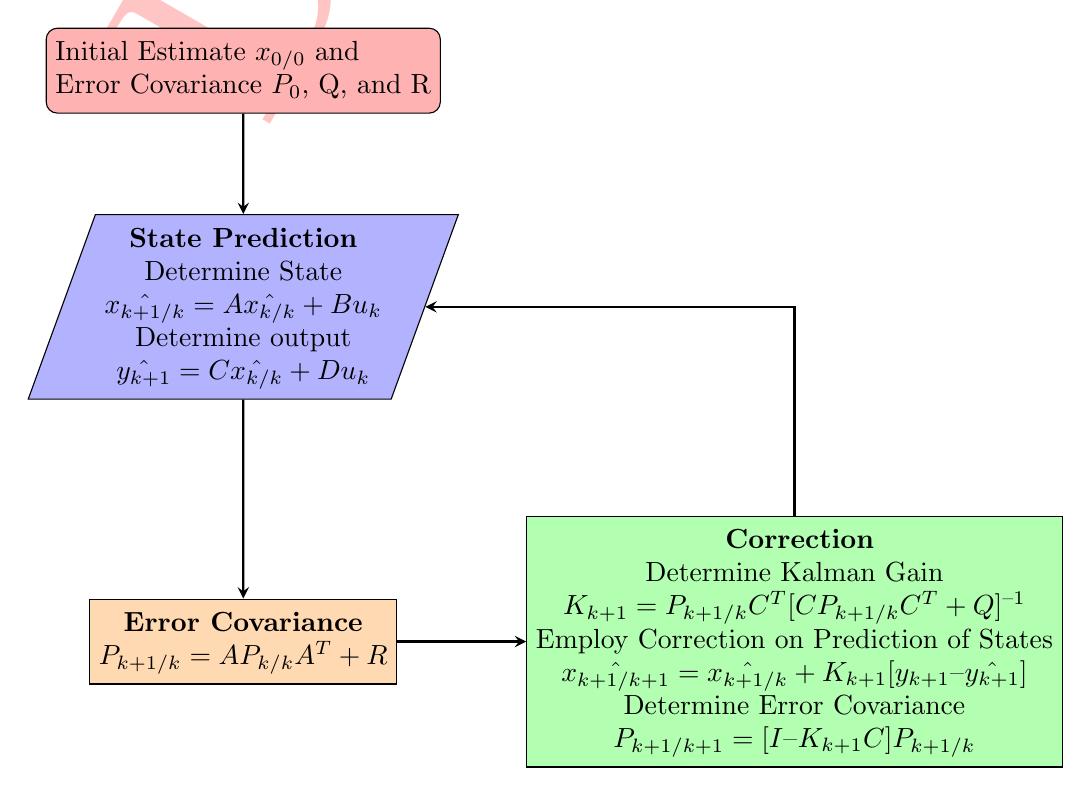
\begin{tikzpicture}[node distance=2cm]
            \node (start) [startstop] {
                \makecell[l]{Initial Estimate $x_{0/0}$ and \\ 
                            Error Covariance $P_0$, Q, and R}
            };
            \node (in1) [io, below of=start,yshift=-1cm] {
                \makecell {
                    \textbf{State Prediction} \\
                    Determine State\\
                    $\hat{x_{k + 1/k}} = A \hat{x_{k/k}}  + B u_k$\\
                    Determine output\\
                    $\hat{y_{k + 1}} = C \hat{x_{k/k}} + D u_k$\\
                }
            };
            \node (pro1) [process1, below of=in1,yshift=-2.25cm] {
                \makecell{ 
                    \textbf{Error Covariance} \\
                    $P_{k + 1/k} = A P_{k/k} A^T + R$\\
                }
            };
            \node (pro2) [process2, right of=pro1, xshift=5cm] {
                \makecell{ 
                    \textbf{ Correction} \\
                   Determine Kalman Gain\\
                   $K_{k + 1} = P_{k + 1/k} C^T [C P_{k + 1/k} C^T + Q]^{–1}$\\
                   Employ Correction on Prediction of States\\
                   $\hat{x_{k + 1/k + 1}} = \hat{x_{k + 1/k}} + K_{k + 1} [y_{k + 1} –  \hat{y_{k + 1}}]$ \\
                   Determine Error Covariance\\
                   $P_{k + 1/k + 1} = [I – K_{k + 1} C] P_{k + 1/k}$\\
                }
            };
            \draw [arrow] (start) -- (in1);
            \draw [arrow] (in1) -- (pro1);
            \draw [arrow] (pro2) |- (in1);
            \draw [arrow] (pro1) -- (pro2);
        \end{tikzpicture}
        \caption{Discrete Kalman Filter Algorithm Flow Chart}
        \label{algo:Discrete_Kalman_Filter_Algorithm_Flow_Chart}
\end{figure}


\begin{itemize}
    \item \textbf{Initialization :} Then the state vector $x_0$ and its associated covariance vector $P_0$ for $K=0$ are initialized. Both perturbations, w and v are uncorrelated white Gaussian random processes with known value covariance matrices Q and R are initialized at this step of the algorithm.
    \item \textbf{Prediction :} For each iteration k newly acquired input data, u is injected into the system, Based on the calculated prior state $\hat{x_{k+1/k}}$, the state vector is predicted along with predicted covariance $P_{k+1/k}$.
\end{itemize}

\begin{equation}\label{eq:Discrete_Prior_State_Equation}
    x_{k+1/k} = A_k x_k + B_k u_k 
\end{equation}
\begin{equation}\label{eq:Discrete_Prior_Covariance_Equation}
    P_{k+1/k} = A_k P_k A_k^{T} + Q
\end{equation}

If the system is stable then $A_k P_k A_k^{T}$ is diminished and reduces the uncertainty of the state estimation over time. The process noise term Q always increases the
uncertainty because $w_k$ cannot be measured. The second estimated $\hat{x_{k + 1/k + 1}}$ tunes up the first estimated $\hat{x_{k + 1/k}}$ (prior state) after measuring the system output $y_k$. The state and error covariance $\hat{x_{k + 1/k + 1}}$ and $P_{k + 1/k + 1}$
are more accurate than $\hat{x_{k + 1/k}}$ and $P_{k+1/k}$ as they involve the information from the measurement $y_k$.

The projected state estimation plus a weighted correction factor  $\hat{x_{k + 1/k + 1}} = \hat{x_{k + 1/k}} + K_{k + 1} [y_{k + 1} –  \hat{y_{k + 1}}]$, as illustrated in, equals the updated state estimation, which is denoted by the symbol $K_k$(Kalman gain).
$P_{k+1/k}$ tends to be "big," which results in a large Kalman gain, which results in a large update for the state estimation $\hat{x_{k + 1/k + 1}}$ if the current state estimation $\hat{x_{k + 1/k}}$is highly uncertain.
The current state estimation will only need to be slightly updated if the current state estimation is confident. Additionally, if the measurement noise is strong due to a high R value, this will result in a low Kalman gain and a little update. The signal to noise ratio (SNR) of the sensor is additionally balanced by the Kalman gain. When the sensor's SNR is high, the Kalman gain is low and the filter converges more quickly.
\begin{itemize}
    \item \textbf{Corretion and Update :} A correction factor ($y_{k + 1} –  \hat{y_{k + 1}}$) equal to the system output $ \hat{y_{k + 1}}$ is added to the new measurement $y_k$ to provide fresh information.
\end{itemize}

The best information on the state and error covariance is used to initialize the Kalman filter, as shown in eq . \ref{eq:Kalam_state_and_covaraince_initialize}.
\begin{equation}\label{eq:Kalam_state_and_covaraince_initialize}
    \hat{x_{k/k}} = E[x_{k/k}], P = E[(x_{k/k} - \hat{x_{k/k}})(x_{k/k} - \hat{x_{k/k}})^T]
\end{equation}
Even though it happens frequently that these quantities are not precisely known, the Kalman filter is well renowned for being extremely resilient to improper initialization and will swiftly converge to the correct values as it runs.


\subsection{Extended Kalman Filter}

The extended Kalman filter is the Kalman filter for nonlinear systems. With the extended Kalman filter technique, a linearization procedure is carried out at each time step to approximate the nonlinear system with a linear time-varying system. The extended Kalman filter for the real nonlinear system is produced by using the linear time-changing system in a Kalman filter. Similar to a Kalman filter, an extended Kalman filter assumes that the process noise and sensor noise are independent, zero-mean Gaussian noises and uses the measured input and output to get the minimum mean squared error estimate of the true state \cite{ADIJ_MARTIN2017}.

In the battery pack system equation\ref{eq:Discrete_OTC_Voltage } and 4.3, the system state variables are defined as $x_1(t) = SOC_0$ and $x_2(t) = V_{OTC}$. The input is defined as u(t) = $i_{batt}$ and the output is y(t) = $V_batt$. 
\begin{equation}
    \dot{x}  = f(x,u) + w
\end{equation}
\begin{equation}
    y  = g(x,u) + v
\end{equation}
where $x = [x_1,x_2]^T$, The functions $f(x,u)$  and $g(x,u)$ are :
\begin{equation}\label{eq:Batt_Kalman_State_function}
    f(x,u) =  \begin{bmatrix}
                    \frac{u}{k C_{OTC}} \\
                    -\frac{1}{R_{OTC} C_{OTC}} x_2 + \frac{1}{C_{OTc}} u
               \end{bmatrix}  
\end{equation}
\begin{equation}\label{eq:Batt_Kalaman_output_function}
    g(x,u) = k x_1 + x_2  + R_0 u + d
\end{equation}
the relationship between battery OCV and SOC is only piecewise 
linear in practice, $V_{OC}$(Open circuit voltage ckt. \ref{fig:Battery_Equivalent_circuit}(b)) can be expressed as 
$V_{OC} = K S_{OC} + d$
$V_{OC}$ could also be a polynomial interpolation of the soc.\\

Recalling the battery terminal voltage from model \ref{fig:Battery_Equivalent_circuit}(b):
\begin{equation}\label{eq:Batt_Kalaman_Terminal_Voltage}
    V_{batt} = K S_{oc} + V_{OTC} - I_{batt} R_0 + d
\end{equation}

If the functions f(x,u) and g(x,u) are linearized by a first-order, Taylor 
series expansion, at each sample step about the current operating point, 
the linearized model is 
\begin{equation}\label{eq:Batt_Kalman_State_function_tylor_expansion}
    \delta \dot{x} = A_k \delta x + B_k \delta u
\end{equation}
\begin{equation}\label{eq:Batt_Kalaman_output_function_tylor_expansion}
    \delta y = C_k \delta x + D_k \delta u
\end{equation}

where ;
\begin{equation}\label{eq:Batt_Kalman_function_tylor_expansion_Ak}
    A_k = \frac{d f(x,u)}{d x} =  \begin{bmatrix}
                                        0 & 0 \\
                                        0 & -\frac{1}{R_{OTC} C_{OTC}} 
                                  \end{bmatrix}                          
\end{equation}
\begin{equation}\label{eq:Batt_Kalman_function_tylor_expansion_Bk}
    B_k = \frac{d f(x,u)}{d x} =  \begin{bmatrix}
                                        -\frac{1}{K Q_{tot}} \\
                                         -\frac{1}{ C_{OTC}} 
                                  \end{bmatrix}                          
\end{equation}
\begin{equation}\label{eq:Batt_Kalman_function_tylor_expansion_Ck}
    C_k = \frac{d f(x,u)}{d x} =  \begin{bmatrix}
                                    K & 1\\  
                                  \end{bmatrix}                          
\end{equation}
\begin{equation}\label{eq:Batt_Kalman_function_tylor_expansion_Dk}
    D_k = \frac{d f(x,u)}{d x} =  [R_0]                         
\end{equation}

The battery model represented by equation \ref{eq:Batt_Kalman_State_function_tylor_expansion} and \ref{eq:Batt_Kalman_function_tylor_expansion_Bk} can be discretized as
\begin{equation}\label{eq:Batt_Kalman_State_Prediction}
    x_{k+1} = A_d x_k + B_d u_k 
\end{equation}
\begin{equation}\label{eq:Batt_Kalman_Output_Prediction}
    y_{k+1} = C_d x_k + D_d u_k
\end{equation}

where $A_d \simeq  E + T_c A_k, B_d \simeq  T_c B_k$, E is the unit matrix and $T_c$ is the sampling 
period, and $C_d \simeq  C_k, D_d \simeq  D_k$ . 
\begin{figure}
    \centering
    \includegraphics[width=0.5\textwidth]{Chap07/Figures/Kalman_principle.PNG}
    \caption{Kalman Filter Principle}
    \label{fig:Kalman_Filter_Principle}
\end{figure}
The Kalman filter is an ideal observer, and Figure \ref{fig:Kalman_Filter_Principle} shows how it works. The idea is to employ a feedback system that modifies the model's uncertain variables to reduce errors between estimated and measured outputs as they occur in real-time. By using a model fit like this, it is feasible to observe the model's physical parameters that are not measurable. The correction allows for the dynamic and functional correction of the filter and is weighted by a gain vector K. Every iteration uses error forecasts and uncertainties (noise) on states and observations to calculate the gain.
The flowchart \ref {algo:Discrete_Kalman_Filter_Algorithm_Flow_Chart} describes the implementation of the extended Kalman filter and I have also grabbed an opportunity to implement the algorithm through the script (described \ref{sec:Extended Kaman Filter Implementation}). 

\section{Extended Kalman Filter Results Discussion}

\subsection{Charging Mode of the LIPO Batteries :}
The Kalman filter experimentation for estimating the soc was carried out on the 10Ah LiPo battery. Figure general charging profile of the LiPo battery, most appropriate charging procedure is to charge the battery in constant current mode as battery voltage reaches close to 4.2Volts change the batteries in the constant voltage (CV) and let the current drop slowly. This charging profile is demonstrated in Figure 2 to estimate the battery soc from the Kalman filter and amper second method. As a result, 1 LIPO battery has reached charged with 4.1Volt with a constant current of 4.5A somewhere around 30 to 40mins, but the soc of the battery is still at $75\%$ to let the battery charge to $100\%$ SOC the charging mode has been a change from CC to CV and the current slowly dropped to zero.
\begin{figure}[h]
	\centering
	\subfigure[Battery Charging Voltages]{\includegraphics[scale=.4]{Chap07/pyKalmanFilter/Python/Figures/BatteryChargingVoltage.png}}
	\qquad
	\subfigure[Battery Charging Current]{\includegraphics[scale=.4]{Chap07/pyKalmanFilter/Python/Figures/BatteryChargingCurrent.png}}
	\qquad
	\subfigure[Battery Charging SOC]{\includegraphics[scale=.4]{Chap07/pyKalmanFilter/Python/Figures/BatteryChargingSOC.png}}
	\qquad
	\subfigure[Battery Charging SOC Error]{\includegraphics[scale=.4]{Chap07/pyKalmanFilter/Python/Figures/BatteryChargingSOCError.png}}
	\caption{Charging Battery Kalman Filter Results}
	\label{fig:Charging_Battery_Kalman_Filter_Results}
\end{figure}

\subsection{Sampling Time $dt$ :}
In an ideological world, we need to sample the current flowing in the battery to calculate the most accurate soc of the battery, but this is quite difficult to do in the practical world, so we need to discretize the time and take the current sample in $T_c$  or $dt$ time.  As we push the sample time smaller and smaller we are close to estimating the actual current flowing in the battery and soc. On the contrary, if we push measurement time to a very very narrow value there is a high chance that to acquire more measurement noise, and we may end up with wrong estimations. This problem is even more emphasized in the column count method,  well than what is the right sample time; it is very hard to say. It depends on the measurement setup and the charging current profile. I have made a few experiments to demonstrate noise encountering the measuring setup and wrong estimations. 

\begin{figure}
    \centering
    \includegraphics[width=0.5\textwidth]{Chap07/pyKalmanFilter/Python/Figures/Charging-curve-for-Lithium-polymer-battery.png}
	\caption{Charging Profile of the LIPO Batteries}
	\label{fig:Charging_Profile_of_the _LIPO_Batteries}
\end{figure}

\subsection{SOC estimation by Kalman Filter:}
SOC estimated by the Kalman filter is quite satisfactory for this LIPO battery the results have been demonstrated \ref{fig:Charging_Battery_Kalman_Filter_Results}(c) and (d). Figure \ref{fig:Charging_Battery_Kalman_Filter_Results}(c) points out the true soc(SOC profile given by the manufacturer), the Coulomb count method, and Kalman filter soc estimation. The green graph is the Coulomb count soc which is acquired with $0.01\%$ of the random noise in the setup, the results have been quite clear that the Coulomb count method keeps on accumulating the noise and diverging from true soc.
On the contrary Kalman filter encounter a lot of noise at the initial stage because the covariance matrix$P_k$ that we initialized might have far diverged from the measuring values in the system (eq . \ref{eq:Discrete_Noise_Covariance}). As time progresses the algorithm will try to correct the error between the true measurement $y_k$ and the estimated value $\hat{y_k}$ and tune its Kalman gain and approaches to the true soc of the battery.

\begin{figure}[h]
	\centering
	\subfigure[Battery Charging SOC @ $dt$=1mS]{\includegraphics[scale=.4]{Chap07/pyKalmanFilter/Python/Figures/BatteryChargingSOC_dt0_01.png}}
	\qquad
	\subfigure[Battery Charging SOC @ $dt$=1mS]{\includegraphics[scale=.4]{Chap07/pyKalmanFilter/Python/Figures/BatteryChargingSOCError_dt0_01.png}}
	\caption{Charging Battery Kalman Filter Results Smaplingtime $dt$ = 1mS}
	\label{fig:Charging_Battery_Kalman_Filter_Results_SamplingTime_1mS}
\end{figure}

Figure \ref{fig:Charging_Battery_Kalman_Filter_Results_SamplingTime_1mS} shows the Kalman and coulomb count soc estimation with a sampling time of 1ms and the error between the true soc to the estimated soc is a lot, even the Kalman filter is oscillating too much to tune the Kalman gain. The Results expressed in figure \ref{fig:Charging_Battery_Kalman_Filter_Results}(c) and (d) are sampled at 100ms with $0.01\%$ measurement noise, the soc estimation is pretty much descent compared to the 1ms results.
The conclusion from this experiment is the sample time Tc is very very important for the SOC estimation even both for the Kalman filter and Ampers second count, but it is not a predefined value it depends on the measurement and data acquisition setup.

\section{Limitations of the Kalman Filter for SoC Estimation }
Undoubtedly Kalman filter is the most robust and well-assimilated approach to calculating the soc mitigate noise, especially in a noisy and dynamic environment. Kalman filter always takes reference from the model(shown in the principle \ref{fig:Kalman_Filter_Principle}) $\hat{y_k}$ and tries to correlate the estimated data from the measuring data $y_k$, but the major drawback in the battery mathematical model is the measuring parameters $R_0,R_{OTC},C_{OTC},V_{OC}$, used to compute the mathematical model no longer holds a direct functional relationship ($V_{OC} = f(SOC) , R_{0} = f(SOC) $ .etc.) with the SOC. They might change over time depending on the battery aging, temperature, and several other environmental factors. For the best convergence of the Kalman filter, we need to initialize $X_{0/0}$ the proper state vector $X_{0/0} = [SOC_0 V_{OTC}]^T$ and input covariance matrix $P_{0/0}$, this is not so simple because the measurement data span $P_{0/0} \in \mathfrak{R}^{N \times N} $ could be much broader and multidimensional.
N could be very large as well, as the N increase (No of batteries in the pack) the computational complexity will increase exponentially with $N \times N$ times for every additional battery that we add to the battery pack.
Implementation of the algorithm in embedded systems for large battery packs makes it vulnerable for the hardware, so small-scale embedded hardware may not be suitable for Kalman filter algorithm implementation.


Synchronization of the measurements in the Kalman algorithm is another deep hit that we can get, for the coulomb count method it is sufficient to synchronize the currents but for the Kalman approach we need both current and voltage measurements should be synchronized this could be another bottom neck for BMS. I have dedicated an entire chapter to explain how difficult is to synchronize the current if voltage synchronization adds up it will double the problem of synchronization.

\section{Future of the Kalman Filter}
Despite the Kalman filter being heavy and slow convergence for small applications, it has proven that over time its robustness helped to mitigate the noise in the system. Nevertheless, the Kalman algorithm can be tweaked to advance machine learning and adaptive algorithms to emphasize its benefits for convergence and light computations. In the following sections, I have summarized the future and updated Kalman algorithms.
\subsection{Unscented Kalman Filter}
It is suggested that UKF be used to address the filtering issue in some really severe nonlinear systems because high orders are disregarded in EKF. The unscented Transform (UT) is used in UKF because it is thought that the probability density of a nonlinear function can be approximated more easily than the nonlinear function itself\cite{Comparision_EKF_UKF_He}.

Assuming x has to mean x and covariance $P_x$, a set of 2n + 1 (n,the state dimension) sigma points can be chosen, which is shown in Equation:

\begin{equation} \label{eq:UKF_state_initialization}
    \begin{split}
    x_0 & = \bar{x} \\
    x_i & = \bar{x}  + (\sqrt{(n+\lambda )P_x} )_i, i\in{1,2,\cdots n}\\
    x_i & = \bar{x}  - (\sqrt{(n+\lambda )P_x} )_i, i\in{n+1, \cdots 2n}\\
    \end{split}
\end{equation}

The collection of dots can roughly represent the state x's Gaussian distribution. Transform all the points nonlinearly: In this stage, all the points would undergo a nonlinear transformation following the nonlinear function.
The results can be expressed as:
\begin{equation} \label{eq:UKF_y_results}
    Y_i = f(x_i)
\end{equation}
The distribution of $y = f(x)$  can be approximately revealed by the set of sigma points {$y_i$}\cite{Comparision_EKF_UKF_He}.

Determine the mean value and covariance of y by doing this calculation.
Following weighting:
\begin{equation} \label{eq:UKF_covariance_initialization}
    \begin{split}
    \bar{y} & \simeq  \sum_{i = 0}^{2n} W_i^{(m)} Y_i  \\
    P_y & \simeq  \sum_{i = 0}^{2n} W_i^{(c)} (Y_i  - \bar{y})(Y_i  - \bar{y})^{T}  \\
    W_0^{(m)} &= \frac{K}{n+k}\\
    W_0^{(c)} &= \frac{K}{n+k} + (1 - \alpha^{2} + \beta  )\\
    W_i^{(m)} &= W_i^{(c)} = \frac{K}{2(n+k)}, i\in{1, \cdots 2n} \\
    \end{split}
\end{equation}

Where $W_i^{(m)}, W_i^{(c)}$ separately the weight factors of the mean value and the covariance.
The above process can be described in Figure \ref{fig:UKF_UT_Transformation}:
\begin{figure}[h]
	\centering
	\includegraphics[width=0.8\textwidth]{Chap07/Figures/UKF_UT.PNG}
	\caption{UKF UT Transformation }
	\label{fig:UKF_UT_Transformation}
\end{figure}
Estimate using the Kalman filter standard: Since the state space for SoC estimation is the same as that for EKF, we can easily demonstrate the unscented Kalman filter technique as follows:


\textbf{Initialization:}\\
\begin{equation} \label{eq:UKF_initialization}
    \bar{x_0} = \textbf{E}(x_0) , P_0 = \textbf{E}[(x_0 - \bar{x_0})(x_0 - \bar{x_0})^{T}] \\
\end{equation}  
State Initialization refers to the equation \ref{eq:UKF_state_initialization}.

\textbf{Time Update:}\\
State estimate time update:  \\
\begin{equation} \label{eq:UKF_State_estimate_time_update}
    x_{k/k-1} = f(x_{k-1},x_{k-1}^{v}), \bar{x_{k/k-1}} = \sum_{i = 0}^{2n} W_i^{(m)}x_{i,k/k-1} \\
\end{equation}  

Error covariance time update: \\
\begin{equation} \label{eq:UKF_Error_covariance_time_update}
    P_{x,k/k-1} = \sum_{i = 0}^{2n} W_i^{(c)}[(x_{i,k/k-1} - \bar{x_{i,k/k-1}})(x_{i,k/k-1} - \bar{x_{i,k/k-1}})^{T}] \\
\end{equation}  

Output estimate time update: \\
\begin{equation} \label{eq:UKF_Output_estimate_time_update}
    Y_{k/k-1}  = g(x_{k/k-1},x_{k/k-1}^{n}),  \bar{y_{k/k-1}}  = \sum_{i = 0}^{2n_a} W_i^{(m)}Y_{i,k/k-1}\\
\end{equation}  

\textbf{Measurement is updated:} \\
Estimator gain matrix: \\
\begin{equation} \label{eq:UKF_Estimator gain matrix}
    \begin{split}
        P_{y,k} & =  \sum_{i = 0}^{2n} W_i^{(c)} (Y_{i,k/k-1}  - \bar{y})(Y_{i,k/k-1}   - \bar{y})^{T}  \\
        P_{xy,k} & =  \sum_{i = 0}^{2n} W_i^{(c)} (Y_{i,k/k-1}  - \bar{x})(Y_{i,k/k-1}   - \bar{y})^{T} \\
        \textbf{K} &= P_{xy,k} \times P_{y,k}^{-1}  \\
    \end{split}
\end{equation}  

State estimate update: \\
\begin{equation} \label{eq:UKF_State_estimate_update}
     \hat{x_k} = \hat{x_k^{-}} + K (y_k - \hat{y_k^{-}} )  \\
\end{equation}  

Error covariance measurement update:\\
\begin{equation} \label{eq:UKF_Error_covariance_measurement_update}
    P_{x,k} = P_{x,k}^{-}  -  K P_{y,k} K^{T} \\
\end{equation}  

The process can be expressed as shown in Figure \ref{fig:SoC_estimation_based_on_UKF}
\begin{figure}[h]
    \centering
    \includegraphics[width=0.5\textwidth]{Chap07/Figures/SoC_estimation_based_on_UKF.PNG}
    \caption{SoC estimation based on UKF }
    \label{fig:SoC_estimation_based_on_UKF}
\end{figure}

\subsection{Adaptive Unscented Kalman Filter}
To determine the battery's SOC, the extended Kalman filter (EKF) was developed. This approach views the SOC as a state variable and may estimate the dynamic system state using the least-squares method. The EKF, on the other hand, is forced to linearize the nonlinear system function using the Taylor series expansion, thus it ignores the high-order elements and invariably makes mistakes. Unscented transform (UT) is used by the unscented Kalman filter (UKF) to handle nonlinear issues. The estimate precision is increased compared to the EKF approach because it doesn't require computing the Jacobian matrix and doesn't overlook high-order terms \cite{Adaptive_UKF_for_SOC_Estimation}.
The particle filter (PF) employs a statistical approach that can be effective for nonlinear issues and does not need that the measurement noise and the observation noise follow a Gaussian distribution, however, this algorithm's computation is complicated.
The strong tracking unscented Kalman filter is used in literature, but to calculate the strong tracking factor, it is also necessary to compute the Jacobian matrix, which increases the computing work.

The UKF (and EKF) algorithm, the strong tracking filter, and the adaptive algorithm are all combined in the adaptive strong tracking unscented Kalman filter (ASTUKF) algorithm. Unlike other strong tracking filters, this method does not need to calculate the Jacobian matrix, which lessens the computational load. This approach can increase tracking and robustness to sudden changes and can fix the SOC estimating mistake brought on by model error [\cite{LIPO_AUKF_Meng},\cite{Comparision_EKF_UKF_He}].

The Adaptive Unscented Kalman Filter forced inherits all the implementation steps from UKF, AUKF takes the approach that the residual sequence remains orthogonal to one another by adding a fading component to the state-prediction covariance matrix and adjusting the gain matrix in real-time. The AUKF method has been refined by literature and no longer requires computing the Jacobian matrix. The battery model mistake can affect the battery's SOC estimation. We employ the AUKF approach as a SOC estimator because it can increase estimate accuracy and decrease SOC estimation error brought on by model imbalance.

The process of determining the fading factor $\gamma _{k+1}$ :\\

\begin{equation}\label{eq:AUKF_fadding_factor}
	V_{k+1}=\begin{cases}
	  e(1)e(1)^{T}, & \text{K=0}.\\
	  \frac{\rho V_k + e(k+1)e(k+1)^{T}}{1 + \rho}, & \text{$K \geq 1$}.\\
	\end{cases}
\end{equation}
Where, $e(k+1) = Y_{k+1} - \bar{Y_{k+1/k}}$, $\rho$ is forgetting factor, $ 0 \leq  \rho \leq 1 $ \\

\begin{equation}
	\begin{cases}
	  N_{k+1} & = V_{k+1} - \beta R_{k+1} \text{where R is Noise covaraince matrix}\\
      M_{K+1} & =  \sum_{i = 0}^{2n} W_i^{(c)} (Y_{i,k+1/k}  - \bar{Y_{k+1/k}})(Y_{i,k+1/k}   - \bar{Y_{k+1/k}  })^{T} \\
	\end{cases}
\end{equation}
\begin{equation}
    \gamma _{0} = \frac{tr N_{k+1} }{ tr M_{k+1}} \\
\end{equation}

\begin{equation}
    \gamma _{K+1}=\begin{cases}
                    \gamma _{0}   & \text{$\gamma _{0}$  > 1}\\
                    1   & \gamma _{0}  \leq 1 \\
    \end{cases}
\end{equation}

Then the state covariance matrix is updated: \\
\begin{equation}
    \begin{cases}
    P_{y_k,y_k}& = \gamma _{K+1} \sum_{i = 0}^{2n} W_i^{(c)} (Y_{i,k+1/k}  - \bar{Y_{k+1/k}})(Y_{i,k+1/k}   - \bar{Y_{k+1/k}  })^{T} + R_k \\
    P_{x_k,y_k}& = \gamma _{K+1} \sum_{i = 0}^{2n} W_i^{(c)} (X_{i,k+1/k}  - \bar{X_{k+1/k}})(Y_{i,k+1/k}   - \bar{Y_{k+1/k}  })^{T} + R_k \\
    P_{k+1/k+1}& = \gamma _{K+1} P_{k+1/k+1} - K_{k+1} P_{y_k,y_k} K_{k+1}^T .\\
    \end{cases}
\end{equation}


The AUKF approach adds a fading component to the state-prediction covariance matrix, which maintains good tracking performance, reduces error brought on by model uncertainty, and dynamically modifies the noise covariance matrix. As a result, the AUKF approach, which combines the benefits of the two algorithms EKF, UKF, and AUKF, can produce estimates with a better degree of accuracy.

In contrast to the conventional UKF, the AUKF untraced Kalman filter integrates the AUKF reasoning process to correct the system's measurement noise on the fly. The covariance of the measurement noise is adjusted using the difference between the theoretical value and the actual value of the measured noise along with AUKF reasoning, and the corrected covariance is then added to the output equation to update the system.

\section{Comparision of Kalman Algorithms Results}
The results from Kalman sub-algorithms are quite elegant, I have made distinguished all the algorithms are Kalman algorithms by their soc estimation and error deviation from the true soc of the battery \ref{fig:Kalman_Algorithms_Battery_Charing_SOC_Comparision}.
I also took an opportunity to summarize \ref{fig:Kalman_Algorithms_Battery_Charing_SOC_Comparision}(b) the error deviation from the true soc to the estimated soc, it is very clear from the results that Columb soc estimation performing very poorly compared to all remaining algorithms. Each Kalman algorithm from the extended Kalman algorithm to the adaptive Kalman algorithm one performs better than the others. Deciding which is best is very much self-explanatory from the distinguished results \ref{fig:Kalman_Algorithms_Battery_Charing_SOC_Comparision}. Thanks to the battery model that is presented in  
chapter \ref{ch:Battery_Modeling_Emulation}, is the fundamental foundation for all the algorithms that we have seen all over. Then there is an obvious question why don't we choose the best algorithm among all, well we can but the problem is if we go for the higher-end algorithms the computational power increases exponentially. And it becomes and bottom neck for the small-scale embedded application. The algorithm once can choose based on the measurement setup, computational power, application use case, and many other factors.
\begin{figure}[h]
	\centering
	\subfigure[Kalman Algorithms Battery Charing SOC Estimation ]{\includegraphics[scale=.4]{Chap07/pyKalmanFilter/Python/Figures/BatteryChargingSOC_Comparriosn.png}}
	\qquad
	\subfigure[Kalman Algorithms Battery Charing SOC Estimation Error Comparision]{\includegraphics[scale=.4]{Chap07/pyKalmanFilter/Python/Figures/BatteryChargingSOCError_Comparrison.png}}
	\caption{Kalman Algorithms Battery Charing SOC Comparision}
	\label{fig:Kalman_Algorithms_Battery_Charing_SOC_Comparision}
\end{figure}

\subsubsection{Convergence of Kalman Algorithms :}
I have summarized the convergence of the algorithms in figure \ref{fig:Kalman_Algorithms_Convergence}, extended Kalman filter is converging slower compare to the adaptive Kalman filter algorithms, let me take a moment to explain what causes them for convergence. In the extended Kalman filter picking the initial condition is very much simple and the convergence matrix is very much diversified from the measuring results in the setup which is why it takes more iterations to get converge. UKF takes a random process approach it selects the mean from the measuring data as the initial state and the variance of the measuring data as the covariance matrix. The AUKF forced the residual sequence to remain orthogonal to each other by adding a fading factor to the state-prediction covariance matrix and adjusting the gain matrix in real-time. The AUKF method has been refined by literature and no longer requires computing the Jacobian matrix. The battery model mistake can affect the battery's SOC estimation. We employ the AUKF approach as a SOC estimator because it can increase estimate accuracy and decrease SOC estimation error brought on by model imbalance.

\begin{figure}[h]
	\centering
	\includegraphics[width=0.6\textwidth]{Chap07/pyKalmanFilter/Python/Figures/KalmanAlgorithms_convergence.png}
	\caption{Kalman Algorithms Convergence }
	\label{fig:Kalman_Algorithms_Convergence}
\end{figure}



\section{Summer of the Chapter \ref{ch:Battery_SOC_Estimation_Algorithms}}
All over in chapter \ref{ch:Battery_SOC_Estimation_Algorithms}, I took an effort to gather focus on the Kalman approach to estimating the soc, is it only the algorithm in the literature well certainly not there are plenty of approaches are there in the literature to estimate the soc of the battery. Then a very obvious question is why Kalman's approach? Well, the answer is it is very immune to noise and accurate estimation, and it has proven most algorithms over decades. As an extension of this topic, we can use much more advanced approaches with Kalman, for instance, fuzzy networks with Kalman filter, support vector machines with Kalman, and many others... I have limited this chapter to 3 or 4 (Amper second, Kalman, EKF, UKF, AUKF) types of algorithms for soc estimation. Even we can look into machine learning, AI, and neural network approaches like the random forest, gradient descent, and stochastic gradient descent, etc. machine learning algorithms are more elegant and robust, but the drawback with those algorithms is we need a large amount of data to characterize the algorithms and tune, perhaps millions of data.  So it is not so easy to go ahead with the machine learning approach in smaller firms. Well, then Kalman's approach is the best among all? Not really it has drawbacks as well, but it holds sufficient grounds for estimating the battery soc.
\thispagestyle{empty}
\cleardoublepage
% % % % % % % % % % % % % % % % % % % % % % % % % % %
% % % % % % % % % % % % % % % % % % % % % % % % % % %
\chapter{Misellaneous}\label{chap:miselleneous}
\section{Chapter \ref{chap:BLE}}
\subsubsection{BLUeNRG-355mc BLE module Layout :}
\begin{figure}[h]
	\centering
	\subfigure[Top layer]{\includegraphics[scale=.4]{Chap_Miselleneous/Chap03_Mise/Figures/BLUeNRG_TOP.PNG}}
	\qquad
	\subfigure[Bottom Layer]{\includegraphics[scale=.4]{Chap_Miselleneous/Chap03_Mise/Figures/BLUeNRG_BOTTOM.PNG}}
	\caption{BLUeNRG-355mc BLE Module Layout}
	\label{fig:BLUeNRG-355mc_BLE_Layout}
\end{figure}

\begin{figure}[h]
	\centering
	\subfigure[Power Supply Layer-1]{\includegraphics[scale=.4]{Chap_Miselleneous/Chap03_Mise/Figures/BLUeNRG_LAYER1.PNG}}
	\qquad
	\subfigure[Signals Layer-2]{\includegraphics[scale=.4]{Chap_Miselleneous/Chap03_Mise/Figures/BLUeNRG_LAYER2.PNG}}
	\caption{BLUeNRG-355mc BLE Module Layout}
\end{figure}
\pagebreak
\subsubsection{Nordic nrf52840 BLE module Layout :}
\begin{figure}[h]
	\centering
	\subfigure[Top layer]{\includegraphics[scale=.4]{Chap_Miselleneous/Chap03_Mise/Figures/Nordic_TOP.PNG}}
	\qquad
	\subfigure[Bottom Layer]{\includegraphics[scale=.4]{Chap_Miselleneous/Chap03_Mise/Figures/Nordic_BOTTOM.PNG}}
	\caption{Nordic nrf52840 BLE module Layout}
	\label{fig:Nordic_nrf52840_BLE_Layout}
\end{figure}

\begin{figure}[h]
	\centering
	\subfigure[Power Supply Layer-1]{\includegraphics[scale=.4]{Chap_Miselleneous/Chap03_Mise/Figures/Nordic_LAYER1.PNG}}
	\qquad
	\subfigure[Signals Layer-2]{\includegraphics[scale=.4]{Chap_Miselleneous/Chap03_Mise/Figures/Nordic_LAYER2.PNG}}
	\caption{Nordic nrf52840 BLE module Layout}
\end{figure}

\begin{figure}[tb]
	\centering
	\makebox[\textwidth]{\includegraphics[width=0.9\paperwidth]{Chap_Miselleneous/Chap03_Mise/Figures/BLUeNRG_Schematic.PNG}}
    \caption{BLUeNRG-355mc BLE Complete Schematic}
    \label{fig:BLUeNRG-355mc_BLE_Complete_Schematic}
\end{figure}


\section{Chapter \ref{ch:Architecture_Active_Balancing_BMS}}

\begin{figure}[tb]
	\centering
	\makebox[\textwidth]{\includegraphics[width=0.7\paperwidth]{Chap_Miselleneous/Chap04_Mise/Figures/LM5170_Typical_ciruit.PNG}}
    \caption{Typical Bidirectional circuit of the LM5170}
    \label{fig:Typical Bidirectional circuit of the LM5170}
\end{figure}

\begin{figure}[tb]
	\centering
	\makebox[\textwidth]{\includegraphics[width=0.8\paperwidth]{Chap_Miselleneous/Chap04_Mise/Figures/Switch_FET.PNG}}
    \caption{STD20NF06L Application typical circuit and package}
    \label{fig:STD20NF06L Application typical circuit and package}
\end{figure}

\begin{figure}[tb]
	\centering
	\makebox[\textwidth]{\includegraphics[width=0.7\paperwidth]{Chap_Miselleneous/Chap04_Mise/Figures/LTC4231.PNG}}
    \caption{LTC4231 Application circuit and the Operational waveform }
    \label{fig: LTC4231 Application circuit and the Operational waveform }
\end{figure}

\subsubsection{ Design Example for the LTC4321 Gate Driver :}
As Design takes the following specifications for the Figure\ref{fig: LTC4231 Application circuit and the Operational waveform } application circuit. The application is rated for a max battery pack voltage of 24V at 5A, $C_L=100\mu F$. UV raising=23V, UV falling = 22V, OV rising = 26V.

Sense Resistor :\\
\begin{equation}\label{eq:LTC_Rsense}
	R_{sense}  = \frac{\Delta V_{sense(CB)(MIN)}}{I_{Inrush}} = \frac{\left(47mV \right)}{\left(2A\right)} = \left(23.5m \Omega\right)
\end{equation}
Use RSENSE = 22.5mΩ for margin. Worst case analog current limit:\\
\begin{equation}\label{eq:LTC_Ilimit_min}
	I_{LIMIT(MIN)} = \frac{\Delta V_{sense(ACL)(MIN)}}{R_{sense}} = \frac{\left(65mV \right)}{\left(23.5m \Omega \right)} = \left(2.89A\right)
\end{equation}
\begin{equation}\label{eq:LTC_Ilimit_max}
	I_{LIMIT(MAX)} = \frac{\Delta V_{sense(ACL)(MAX)}}{R_{sense}} = \frac{\left(90mV \right)}{\left(23.5m \Omega \right)} = \left(4A\right)
\end{equation}
Calculate the worst-case time it takes to charge up CL analog current limit:\\
\begin{equation}\label{eq:LTC_Tcharge_max}
	t_{CHARGE(MAX)} = \frac{ C_{L}\times V_{IN}}{I_{LIMIT(MIN)}} = \frac{\left(100\mu F \times 24V \right)}{\left(2.89A \right)} = \left(0.9ms\right)
\end{equation}
For inrush control using analog current limit, $t_{CHARGE(MAX)}$ must be less than the circuit breaker delay (tCB) for a proper start-up \cite{LTC4231_User_Datasheet}.

The worst-case power dissipation in MOSFET M1 occurs "\\
\begin{equation}\label{eq:LTC_Pdissp}
	P_{DISS} = V_{IN} \times I_{LIMIT(MAX)}  = \left(24V \times 4A\right) = \left(96W\right)
\end{equation}

during a severe overcurrent fault when the current is controlled by analog current limit for the duration of tCB:
\begin{equation}\label{eq:LTC_Ct}
    C_{T} = \frac{ t_{Cb}}{24V} = \frac{\left(2mS \right)}{\left(24V \right)} = \left(82nF\right)
\end{equation}

If a low inrush current ($< \Delta V_{SENSE(CB)}$) is preferred, refer
to the Figure \ref{fig: LTC4231 Application circuit and the Operational waveform } application circuit which uses a gate capacitor CG to limit the inrush current. Choose IINRUSH = 0.5A
which is set using $C_G$ \cite{LTC4231_User_Datasheet}:

\begin{equation}\label{eq:LTC_Cg}
	C_{G} = \frac{ C_{l}\times 10\mu A}{I_{Inrush}} = \frac{\left(100\mu F \times 10\mu A \right)}{\left(2.89A \right)} = \left(20nF\right)
\end{equation}
The time to charge up CL with 0.5A is:
\begin{equation}\label{eq:LTC_Tcharge}
    t_{CHARGE(MAX)} = \frac{ C_{L}\times V_{IN}}{I_{Inrush}} = \frac{\left(100\mu F \times 24V \right)}{\left(0.5A \right)} = \left(48ms\right)
\end{equation}
The average power dissipation in the MOSFET M1 during this start-up is:
\begin{equation}\label{eq:LTC_Pdissp_average}
    P_{DISS} = V_{IN} \times I_{LIMIT(MAX)}  = \left(24V \times 0.5A\right) = \left(6W\right)
\end{equation}

\begin{figure}[h]
	\centering
	\includegraphics[width=0.4\textwidth]{Chap04/Figures/Type2a_ABMS.PNG}
	\caption{\textit{Type Ib} Active Balancing Circuit} 
	\label{fig:Type1b Active Balancing Circuit }
\end{figure}

\begin{figure}[h]
	\centering
	\subfigure[Single operation bidirectional buck-boost converter (Low-side)]{\includegraphics[scale=.5]{Chap_Miselleneous/Chap04_Mise/Figures/Bi_buck_boost_low_side.PNG}}
	\qquad
	\subfigure[ Single operation bidirectional buck-boost converter (High-side)]{\includegraphics[scale=.5]{Chap_Miselleneous/Chap04_Mise/Figures/Bi_buck_boost_High_side.PNG}}
	\caption{Typical Schematics of the Low side and High Side buck-boost Converter}
	\label{fig:Typical Schematics of the Low side and High Side buck boost Converter}
\end{figure}
\section{Chapter \ref{ch:Battery_Modeling_Emulation}}
\subsection{Chroma SCPI Commands Example Programs}
The following programming is a raw program that we can do through NI drivers. 

\paragraph{Example 1:} The following commands in example 1 simulate a BMS containing 16 independent batteries with sampling 10ms and current range to 5A. The initial voltage of the 16 batteries is 3.8V/2A and remains 0.5 second after output. When the voltage changes to 4.2V/3A and remains for
0.5 second, it reports the first 100 records of battery 1 and 2, and then turn off the output'\cite{Chroma_UserManual}.
\\\\
\noindent $*IDN?$ \\
$SYSTem:FRAME:STATe?$ 0\\
$SYST:FRAME?$ 0\\
$SYST:FRAME:CHAN:STAT?$ 0\\
$SYST:FRAME:CHAN:NUMB?$ 0 \\
$SYST:ERR?$\\
$SYSTem:ERRor?$\\ 
$SYST:FRAME:PROT:CLE$\\
$SIM:CONF:BMS:NUMB$ 1\\ 
$SIM:CONF:BMS:NUMB?$ \\
$SIM:CONF:SAMP:TIME$ 10\\ 
$SIM:CONF:SAMP:TIME?$\\ 
$SIM:CONF:CELL:NUMB$ 1,16\\
$SIM:CONF:CELL:NUMB?$ 1\\
$SIM:CONF:CELL:PARA$ 1,1,16,1,2\\
$SYSTem:ERRor?$\\ 
$SIM:PROG:CELL$ 1,1,1,16,3.8,2\\
$SIM:OUTP ON$\\
$SYSTem:ERRor?$ \\
$SIM:OUTP?$\\
$*D$ 500\\
$SIM:PROG:CELL$ 1,1,1,16,4.2,3\\
$SYSTem:ERRor?$\\ 
$SIM:OUTP:IMM$\\
$SYSTem:ERRor?$\\
$*D$ 500\\
$SIM:REP:CELL:REC:DATA?$ 1,1,1,100\\
$SIM:REP:CELL:REC:DATA?$ 1,2,1,100\\
$SIM:OUTP OFF$\\
$SYSTem:ERRor? SIM:OUTP?$\\


\paragraph{Example 2:} The following commands in example 2 simulate a BMS containing 16 independent batteries that are paralleled into 8 separate batteries with sampling 10ms and a current range of 5A. The voltage of the 8 batteries is 4.2 V/2A, and it performs measurement 1 second after output. It returns the instant voltage, current and protection status of BMS 1 8 batteries, and turns off the output after 10 seconds.
\\\\
$*IDN?$ \\
$SYSTem:FRAME:STATe?$ 0\\
$SYST:FRAME?$ 0\\
$SYST:FRAME:CHAN:STAT?$ 0\\
$SYST:FRAME:CHAN:NUMB?$ 0 \\
$SYST:ERR?$\\
$SYSTem:ERRor?$\\ 
$SYST:FRAME:PROT:CLE$\\
$SIM:CONF:BMS:NUMB$ 1\\ 
$SIM:CONF:BMS:NUMB?$ \\
$SIM:CONF:SAMP:TIME$ 10\\ 
$SIM:CONF:SAMP:TIME?$\\ 
$SIM:CONF:CELL:NUMB$ 1,16\\
$SIM:CONF:CELL:NUMB?$ 1\\
$SIM:CONF:CELL:PARA$ 1,1,8,2,2\\
$SIM:OUTP ON$\\
$SYSTem:ERRor?$ \\
$SIM:OUTP?$\\
$*D $1000\\
$SIM:MEAS:BMS:VOLT?$ 1\\
$SIM:MEAS:BMS:CURR?$ 1\\
$SIM:MEAS:BMS:PROT?$ 1\\
$*D $10000\\
$SIM:OUTP OFF$\\
$SYSTem:ERRor?$\\
$SIM:OUTP?$\\


\begin{figure}[h]
	\centering
	\subfigure[4 Channel keysight N6705 Power Supply]{\includegraphics[width=0.3\textwidth]{Chap06/Figures/keysight_n6705.PNG}}
    \qquad
	\subfigure[Chroma Output Wiring to the BMS]{\includegraphics[width=0.3\textwidth]{Chap06/Figures/DMM_34460A.PNG}}
	\caption{ keysight N6705 Power Supply and DMM 34460A }
	\label{fig:keysight_n6705_DMM_34460A}
\end{figure}

\begin{figure}[h]
	\centering
	\subfigure[16CH Battery Cell Simulator 87001]{\includegraphics[width=0.3\textwidth]{Chap06/Figures/Chroma.PNG}}
    \qquad
	\subfigure[Chroma Output Wiring to the BMS]{\includegraphics[width=0.3\textwidth]{Chap06/Figures/Chroma_Output_wiring.PNG}}
	\caption{16CH Battery Cell Simulator 87001}
	\label{fig:Chroma}
\end{figure}


\section{Chapter \ref{ch:Battery_SOC_Estimation_Algorithms}}
\subsection{Extended Kaman Filter Implementation}\label{sec:Extended Kaman Filter Implementation}

\begin{lstlisting}[language=Python, caption=Extended Kalaman Filter Script]  
class ExtendedKalmanFilter(object):
    def __init__(self, x, A, B, P, Q, R, Hx, HJacobian):
        self._x = x
        self._A = A
        self._B = B
        self._P = P
        self._Q = Q
        self._R = R
        self._Hx = Hx
        self._HJacobian = HJacobian

    def update(self, z):
        P = self._P
        R = self._R
        x = self._x
        # H Jacobian of Matrix C and D
        H = self._HJacobian(x)
        S = H * P * H.T + R
        #K is the Kalman Gain 
        K = P * H.T * S.I
        self._K = K
        hx =  self._Hx(x)
        y = np.subtract(z, hx)
        self._x = x + K * y

        KH = K * H
        I_KH = np.identity((KH).shape[1]) - KH
        self._P = I_KH * P * I_KH.T + K * R * K.T
    def predict(self, u=0):
        self._x = self._A * self._x + self._B * u
        self._P = self._A * self._P * self._A.T + self._Q
    @property
    def x(self):
        return self._x
\end{lstlisting}
\thispagestyle{empty}
\cleardoublepage
% % % % % % % % % % % % % % % % % % % % % % % % % % %
% % % % % % % % % % % % % % % % % % % % % % % % % % %
\chapter*{Conclusion}
Undoubtedly it's been a wonderful time all over my thesis period. Now it's time to conclude my thesis and make some takeaways from it. The idea of my thesis much diversified and multidisciplinary. Throughout the project, I have entirely dedicated myself to understanding every problem statement we encountered and bringing it to the team. It has been a joyful moment that every problem in the process, gave me intellectual knowledge to think in terms of hardware and software perspective.

Since my thesis is multidisciplinary I partitioned each disciplinary chapter by chapter. I would follow the same approach in the following section to conclude my thesis in each discipline, which includes hardware, software, and even design.

\section*{Chapter \ref{chap:BLE}}
Chapter \ref{chap:BLE} took more space in terms of the RF environment design for the BMS. The Chapter includes Bluetooth module design, Antenna design, RF layout design, etc. In this chapter, I have covered how to pick Bluetooth solutions for BMS applications and what factors we need to keep in mind to select a Bluetooth solution. So far so forth picking a BLE solution was successful, and I have ended with BLUeNRG355 and Nordic Bluetooth stacks. What I have not strongly assured, is why only BLUeNRG355 and Nordic. Well it's not obligatory to go to only these two solutions we have plenty of BLE solutions in the market and the reason behind selecting these two solutions are they are well-established in the Bluetooth world and their documentation is very much self-explanatory.
Users can select any BLE stack depending on their application requirements I have opted for these two solutions based on the project requirements.

Later sections in chapter 1 talk about antenna selection and antenna designing, what makes the reader disconnected from this section? Is mathematical design of the antennas.. Yes I have not included the mathematical calculations because in the proper solutions it is hard to pick new experimental RF antenna shapes the intent of this project purely was to make the BLE communication-based BMS and the main motive was to bring up the nice RF layout using the proprietary solutions. Keeping these requirements in mind I have picked standard MIFA and PIFA antennas and I took an opportunity to guide a reader to literature for more design theory. Yet, I have not missed a chance to discuss the results and compare different antenna results for picking the right antenna for BMS applications.

Further, sections in Chapter 1 are explored in much more detail the RF layout design and precautions we need to take to prevent the RF layout affecting from parasitic components.
After looking at Bluetooth much deeper we should relate this solution to the BMS, which is the most beautiful combination. I have tried to integrate the BLE module with the existing setup, which came out as a very successful solution for the BMS.

\subsection*{Future of BLE in BMS}
So far and so forth BLE proved it is the most reliable solution to the BMS application, but I don't suggest users rely only on the BLE solution. We can be much more explorers with different disciplines like Wi-Fi, Zigbee, and even other proprietary protocols.
I have not stressed the security of BLE, the data management, and square in the BLE these are the topics that could open new doors in the BLE world for the BMS. There is also an open opportunity to explore the BLE integrating with the onboard solution of the BMS (now it is a module-based approach). Doing this could challenge the existing BLE layout and BMS ckt's(due to the parasitics, noise, and power supply issues even many other issues). Nevertheless, the proposed BLE stack and design strategies sustained strong and consistent for our BMS application.

I have a very interesting research idea to test this BLE solution with a large setup and the real battery module setup, like in EV battery packs and I could see the new situation (interference, reflections, etc...) and how reliable this solution could be. Since this is not the scope of my project, I will leave this enthusiastic idea for my future research.
\section*{Conclusion of Chapter \ref{ch:Architecture_Active_Balancing_BMS}}
Chapter \ref{ch:Architecture_Active_Balancing_BMS} is the core of this thesis, which describes the hardware setup for the wireless communication BMS. Since the hardware circuit of the BMS has a lot of subcircuits like auxiliary power supplies, charge pumps, ADC and communication circuits ...etc. I have limited my focus to explaining the main hardware blocks which address the active balancing BMS.

The main blocks involved in the active balancing of the batteries are buck-boost DC/DC converter, BLE, switch matrix, and controller. I have paid close attention to every circuit and the descriptions of the components. For active balancing in this project, I have limited my focus to particular hardware setup and topology (Type 2a pack to cell and vice versa). Still, I attempted to touch each topology flavor at least theoretically. Nonetheless, we can follow any of the active balancing topologies which I have described in chapter 2. Picking the active balancing topology is completely an independent choice for the user based on the application. This chapter took quite a long trip across different hardware and working principles of each circuit .... overall the trip went very successfully because it summarized all the hardware concepts of the active balancing for the batteries.

Active balancing can be expensive for low-level battery applications, but it can save a  lot of energy if we consider large applications like EVs.
\section*{Conclusion of Chapter \ref{ch:Current_Measurement}}
The current measurement chapter \ref{ch:Current_Measurement} is sweet and short, but it is essential for this project. The overall active balancing concept depends on the battery soc and the soc is directly dependent on the $i_{batt}$.

The focal point of this chapter is to measure the current flowing in/out to the battery and synchronize measurement acquisition. In reality, this is not a big problem when we are at an integrated circuit solution because we might have a dedicated sensor for the current sense, and we can spare N number of peripherals to read/write data. All current sensors in the IC are synchronized with the master clock. Since this project is implemented at a discrete level it is hard to synchronize multiple discrete current sensors at the same time.
Keeping these scenarios in mind I came up with two different algorithms to synch the current measurements a) Parallel write and sequential read, b) Delayed measurements. The parallel write and sequential read algorithms are very classical, writing all the sensors at the same time by keeping their i2c address the same after they acquired current measurements simultaneously, changing the address of the sensor by their address lines, and reading them sequentially.
This approach could be very simple and elegant, practically this works fine, but I have not employed this procedure in this project. OK!, let me make out some scenarios and see whether this algorithm stands. For instance, while writing sensors simultaneously master does not care whether it has received acknowledgment from all the slaves are not, it simply receives an acknowledgment from any one slave, and it will continue the writing process. If anyone sensor dropped in between that could be a dangerous situation because the master doesn't know what is happening until it will try to read the measurements. By the time master read the current measurements the balancing has been already started, so we could be in trouble if it does not know how much current was flowing. It is a great approach, but it makes less confidence for my application, but till I support this algorithm if there are low-priority measurement applications.
\\\\
The second approach that stepped in is the delayed approach, but this is a completely application-dependent approach. I got the privilege of selecting the INA2XX series to shunt current sensors, they have the feature of programming a delay. I program current sensors with particular delays to align all the measurements and start acquiring data at the same time. The delay is included with reading and writing time as well.
\\\\
I have employed both approaches they work amazingly fine. I do not have a cent percent assurance whether they work universally for applications or not. Yet, they hold strong ground to synchronize the current measurements for BMS applications.

\section*{Conclusion of Chapter \ref{ch:Battery_Modeling_Emulation}}

Batteries are one of the greatest inventions for mankind, and they have two kinds of views they can be greatest to decrease global warming, and they can be more dangerous if you do not handle them properly. Since batteries are more hazardous in terms of chemicals, and they are very sensitive to the voltages it is essential to give little extra care. It is more often engineers who work on BMS need to do a lot of testing on the batteries and there is a high chance that engineers can encounter some unpleasant events. So, the BMS engineers come up with something beautiful, more effective, and less dangerous. Chapter \ref{ch:Battery_Modeling_Emulation} attempted to address this issue. The proposal was to model the battery as a real battery and emulate it with the lab setup.
\\\\
I have partitioned chapter 4 into two parts first is battery modeling, and the second is implementing the lab setup. The battery modeling section is very much descriptive it explains from scratch how to model the battery and brings up the model parameters from the soc characteristics graph. It is gorgeous, I love the way the battery is modeled with the known circuit components. Not an exaggeration I went through the simple resistive model to the two-time constant model, the future of this modeling could go even high for more accurate battery modeling.\\\\
\\
Part II of chapter 4 is completely based on part I, implemented in the lab setup. I have proposed a power analyzer architecture for the most robust battery modeling and testing in the lab setup. The battery model implementation took place entirely with the python script. The results of this implementation were phenomenally interesting, I took quite a long word to elaborate on the results, please have look.\\
The power analyzer implementation is taken place through the script, but it is not obligatory to go only through this script it is the user's choice. They can make an independent decision, I set up this script based on the instruments that are available to me. The users can make scripts depending on the instruments in their lab, but the power analyzer architecture holds good universally for all BMS lab testing.\\

I have only described major configurations for instruments since scripts take loads of coding lines I have uploaded all the scripts to GitHub and addressed respective links in the miscellaneous.


\section*{Conclusion of Chapter \ref{ch:Battery_SOC_Estimation_Algorithms}}

Chapter \ref{ch:Battery_SOC_Estimation_Algorithms} is the most decorative and lavishing chapter. This chapter employs all the chapters that I have described previously. And the 5th chapter concludes the soc estimation algorithms. It also addresses the most advanced alorithms with descriptive math.

The first few sections made an effort to explain the classical coulomb counting approach and its drawbacks of it. Later sections address resolving the noise problems seen in the coulomb count method through the Kalman approach. Kalman algorithm took a bit of a long approach to resolve the soc estimation issue and converged to the real soc. Nonetheless, it opened new doors for upgraded algorithms like EKF, UKF and AUKF.

Sub Kalman algorithms(EKF, UKF, and AUEKF) that I have discussed in chapter 5 are not only the algorithms left for soc calculations. There is a wide ocean of algorithms is there to explore in the machine learning and AI field. I made a clear attempt to differentiate in the 5th chapter the benefits and drawbacks of using AI due to a lack of data. Nonetheless, I would like to see my future research more on AI and neural networks for EVs.

\section*{Resting the Thesis}

It was a wonderful journey of over a year working on this project. I have seen a lot of ups and downs during the project execution. I would love to thank every person who was on this journey. Furthermore, \textbf{ \textit{I would pledge myself to entitle to technology in the favor of mankind and I ensure whatever I have written in this thesis is true to the best of my knowledge. Now it is the moment to end this thesis. " That's all I will reset my argument here", Thank you!}}
\thispagestyle{empty}
\cleardoublepage
% % % % % % % % % % % % % % % % % % % % % % % % % % %
% % % % % % % % % % % % % % % % % % % % % % % % % % %
\bibliographystyle{Ref/IEEEtran}
% \bibliographystyle{IEEEtran}
% %%%\bibliographystyle{Ref/asme}
% %%%\bibliographystyle{Ref/bmes}
% %%%\bibliographystyle{Ref/achemso}
% %%%\bibliographystyle{Ref/rsc}
% %%%\bibliographystyle{Ref/osajnl}
% %%
% %%%\bibliographystyle{unsrtnat}
\bibliography{Ref/SampleReferences}
% {
% 	\fontsize{10}{12}
% 	\selectfont
% 	\addcontentsline{toc}{chapter}{References}
% 	\bibliography{Ref/SampleReferences}
% 	\footnotetext{This reference format follows ASME style. You are advised to follow one reference format of any dominant journal of your field.}
% }
\cleardoublepage
%%% % % % % % % % % % % % % % % % % % % % % % % % % % %
%%% % % % % % % % % % % % % % % % % % % % % % % % % % %
% \rhead{\textit{Dissemination}}
% \lhead{}
% \SpecialTitle{Dissemination}


\paragraph{Internationally indexed journals} (\textit{Web of Science, SCI, Scopus, etc.})\footnote{\label{published}Articles already published, in press, or formally accepted for publication.}
\begin{itemize}
\item[1.]
\item[2.]
\end{itemize}  

\paragraph{Other journals and Book chapters}\footnotemark[\ref{published}]
\begin{itemize}
\item[1.]
\item[2.]
\end{itemize}  

\paragraph{Conferences}\footnotemark[\ref{published}]
\begin{itemize}
\item[1.]
\item[2.]
\end{itemize}  

\paragraph{Article under preparation}\footnote{\label{unpublished}Articles under review, communicated, or to be communicated.}
\begin{itemize}
\item[1.]
\item[2.]
\end{itemize}  
%
%\begin{itemize}
%\item[]\textbf{Internationally indexed journals}
%\item[1.]
%\item[2.]
%  
%\item[]
%
%\item[]\textbf{Conference Presentations}
%\item[1.]
%\item[2.]
%\item[]
%
%\item[]\textbf{Book Chapters}
%\item[1.]
%\item[2.]
%\end{itemize}

% \thispagestyle{empty}
% \cleardoublepage
% % % % % % % % % % % % % % % % % % % % % % % % % % %
% % % % % % % % % % % % % % % % % % % % % % % % % % %
\indexColumns{3}
\indexPage
% % % % % % % % % % % % % % % % % % % % % % % % % % %
% % % % % % % % % % % % % % % % % % % % % % % % % % %
\end{document}
